\pagebreak
\section{Results}
%\add[XT]{choose some points in the model domain like Choi 2008 did, to monitor the values changes with time (e.g. In VisIt use Query to obtain stress with time for quantatatively analyzing the model behaviors)}
%In this ``Results'' chapter, I first walk through the reference model (M28LinT1) and compare it with a constant M model (M88ConT2). Then, I describe in detail the seven major characteristics of the models. Finally, I describe the effects of different weakening rates, ranges as well as functional forms of M variation on the main characteristics.

\subsection{Reference model}\label{sec_M28LinT1}

I consider the model with M varying linearly from 0.2 to 0.8 along the ridge axis with type 1 weakening rate as the reference model and denote it as M28LinT1 following the shorthand notations given in Table~\hyperref[Tab1_1]{\ref{Tab1_1}}. I describe the general model behaviors in this section and then provide details and mechanisms of the major structural features of the model in the next section.

%The structural features include breakaway (Figure~\hyperref[fig_Results1_1]{\ref{fig_Results1_1}.c}); oceanic core complex (OCC) (Figure~\hyperref[fig_Results1_1]{\ref{fig_Results1_1}.d}); termination of the detachment fault along the ridge where the active faulting interface reaches the seafloor (black dashed lines); new high angle normal faults forming near the ridge axis (Figure~\hyperref[fig_Results1_1]{\ref{fig_Results1_1}.f}), which is termed as ``inward fault jump'' (\citealp{Tucholke1998}); corrugations (Figure~\hyperref[fig_Results1_1]{\ref{fig_Results1_1}.f}) and mullion structures (Figure~\hyperref[fig_Results1_1]{\ref{fig_Results1_1}.g}); and the side-by-side ``brother domes'' (Figure~\hyperref[fig_Results1_1]{\ref{fig_Results1_1}.h}).

For the first 7.5 kyr (Figure~\hyperref[fig_Results1_1]{\ref{fig_Results1_1}.a}), %high angle ($\sim$60 $\degree$)
normal faults, represented by localized plastic strain, begin to form near the ridge axis.
%The angles of the faults are consistent with  Anderson's theory of faulting mechanics for a frictional angle of 30 $\degree$.
Because stresses due to plate extension accummulate faster at the lower M side than at the higher M side, faults first initiate at the lower M side and then propagate to the higher M side. Such an asynchronous initiation of faults along the ridge axis creates offset in breakaway at later stages, i.e., the breakaway at the lower M side moves further away from the ridge axis than that of the higher M side (Figure~\hyperref[fig_Results1_4]{\ref{fig_Results1_4}}).

\begin{figure}[h]
  \centering
    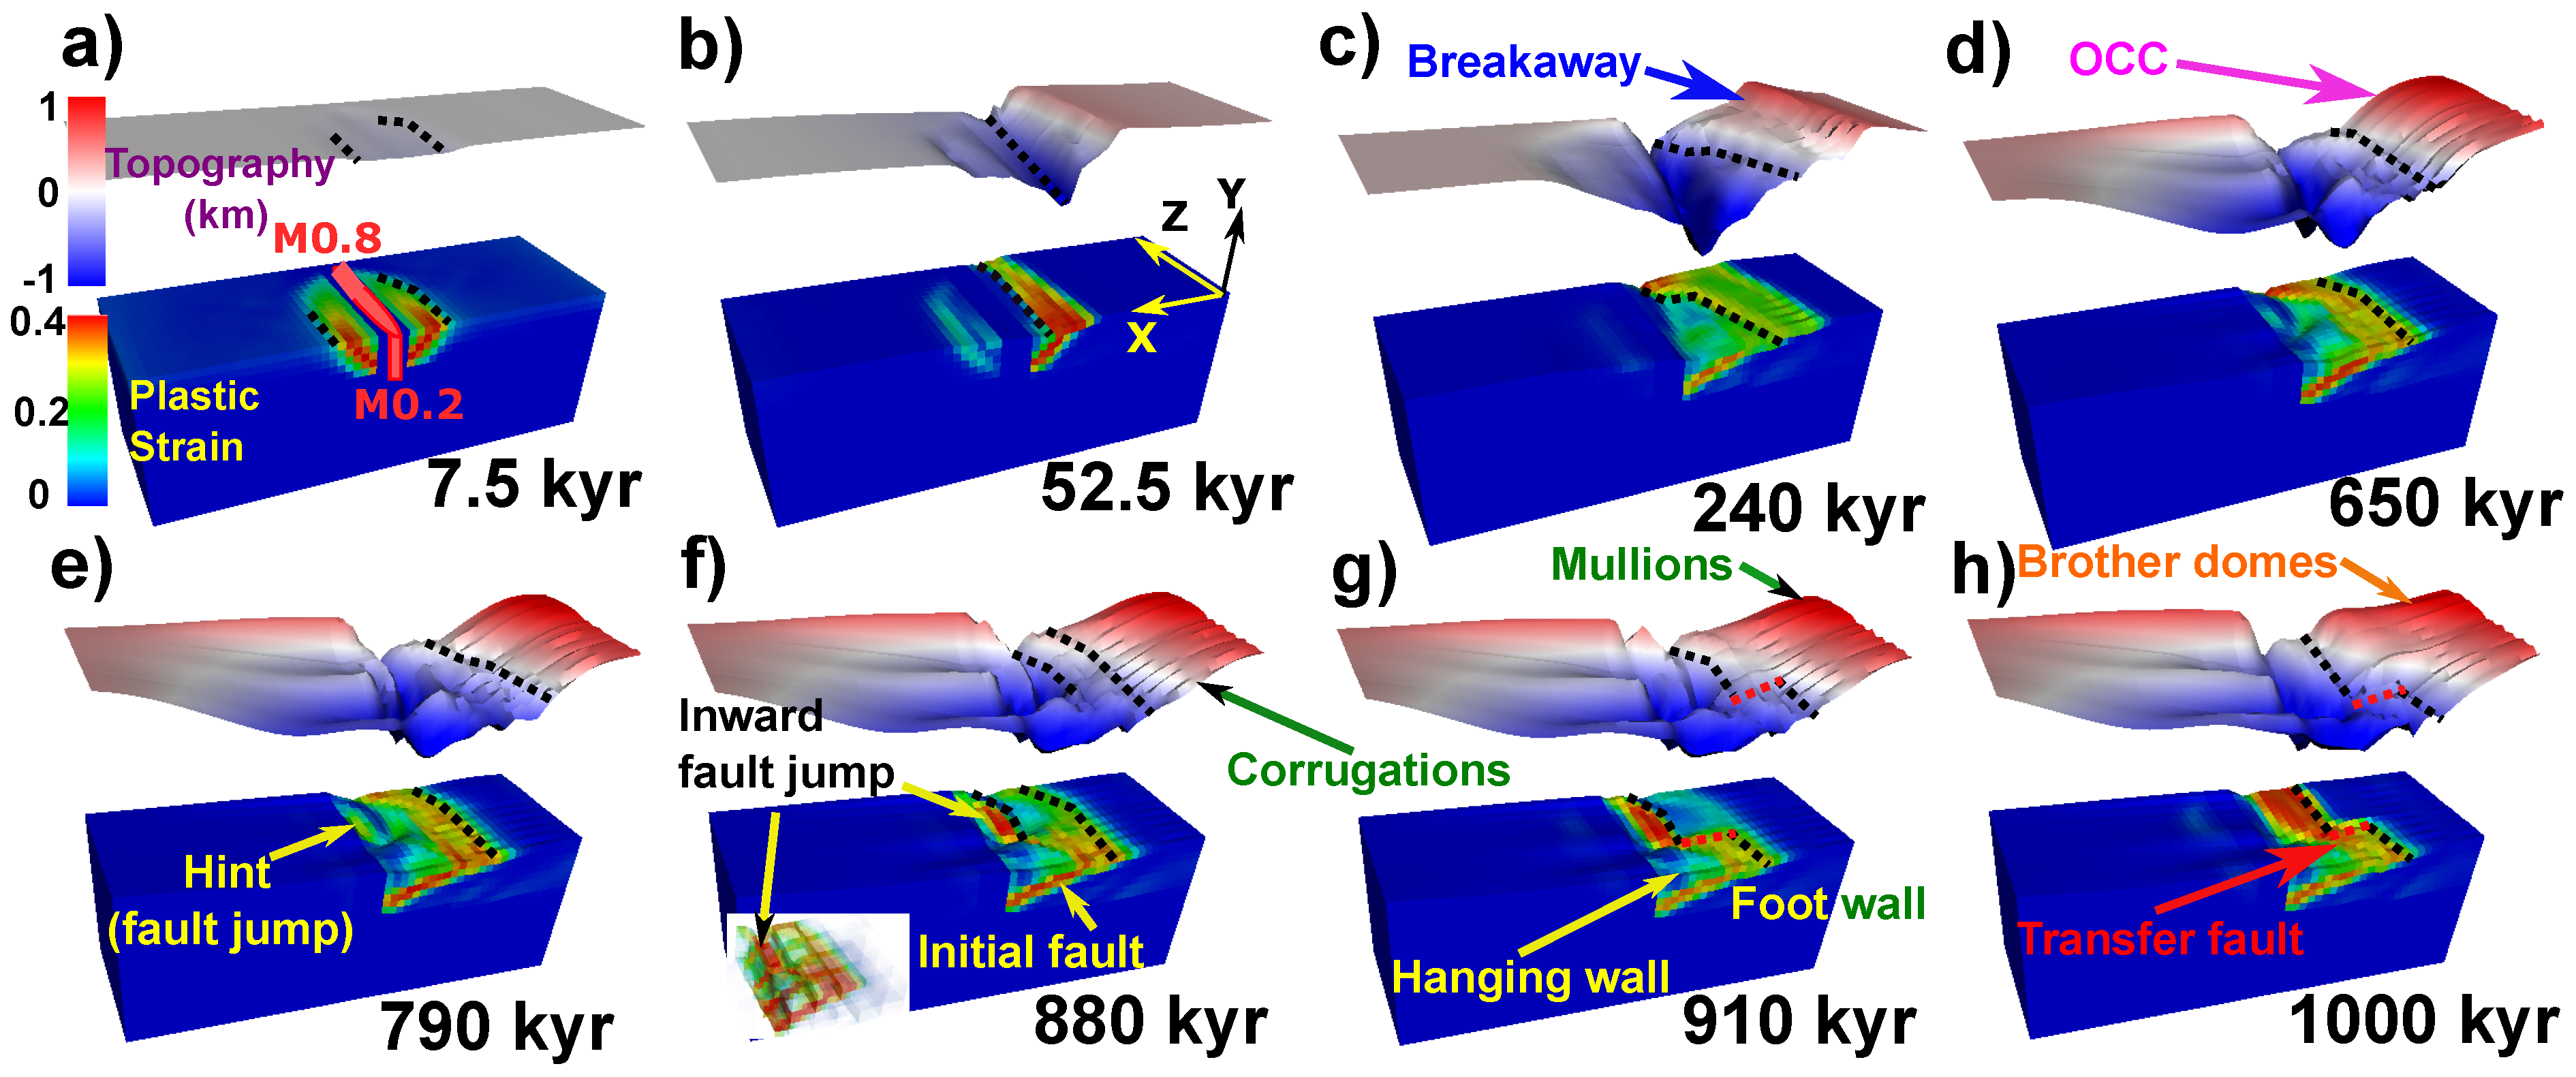
\includegraphics[width=1.0\textwidth]{./Figures/fig_Results_1_reference_model.eps}
  \caption[Reference model M28LinT1.]{Evolution of plastic strain and surface topography of the reference model M28LinT1. Each snapshot shows plastic strain plotted on the model domain, the five times vertically exaggerated topography and the time at which it is taken. The initial seafloor is at 0 km of elevation. The black dashed lines are the terminations of faults. The red dashed lines in g) and h) are the transfer faults that connect the terminations. The inset in f) plots plastic strain with opacity linearly proportional to plastic strain value.}%The two insets in b) and d) show $\sigma_{xx}$ (Sxx in the figure) with positive values meaning  tension. The inset in Figure~\hyperref[fig_Results1_1]{\ref{fig_Results1_1}.h} is for shear stress $\sigma_{xz}$ (Sxz in the figure).  The inset in g) also shows velocity vectors.} %Indicated by the velocity vector, the hanging wall of the detachment fault at low M region (M = 0.2$\sim$0.5) is moving in an opposite direction (negative $x$-axis) to its ajacent higher M region (M $>$ 0.5).} %\note[XT]{one thing to be noted is that the $dt=0.5yr$ in these series of 3D models, thus I divided the time step by two to get the time (kyr). This figure needs to be revised that the plastic strain scale is actually changing for different time, a way to revise it is to maintain a constant color scale or attach a color scale for each time. Also, it seems a little bit small and two rows is not as preferable as one row or one column to better express the concept of linear time series evolution.}}
 \label{fig_Results1_1}
\end{figure}   

\begin{figure}[h]
   \centering
     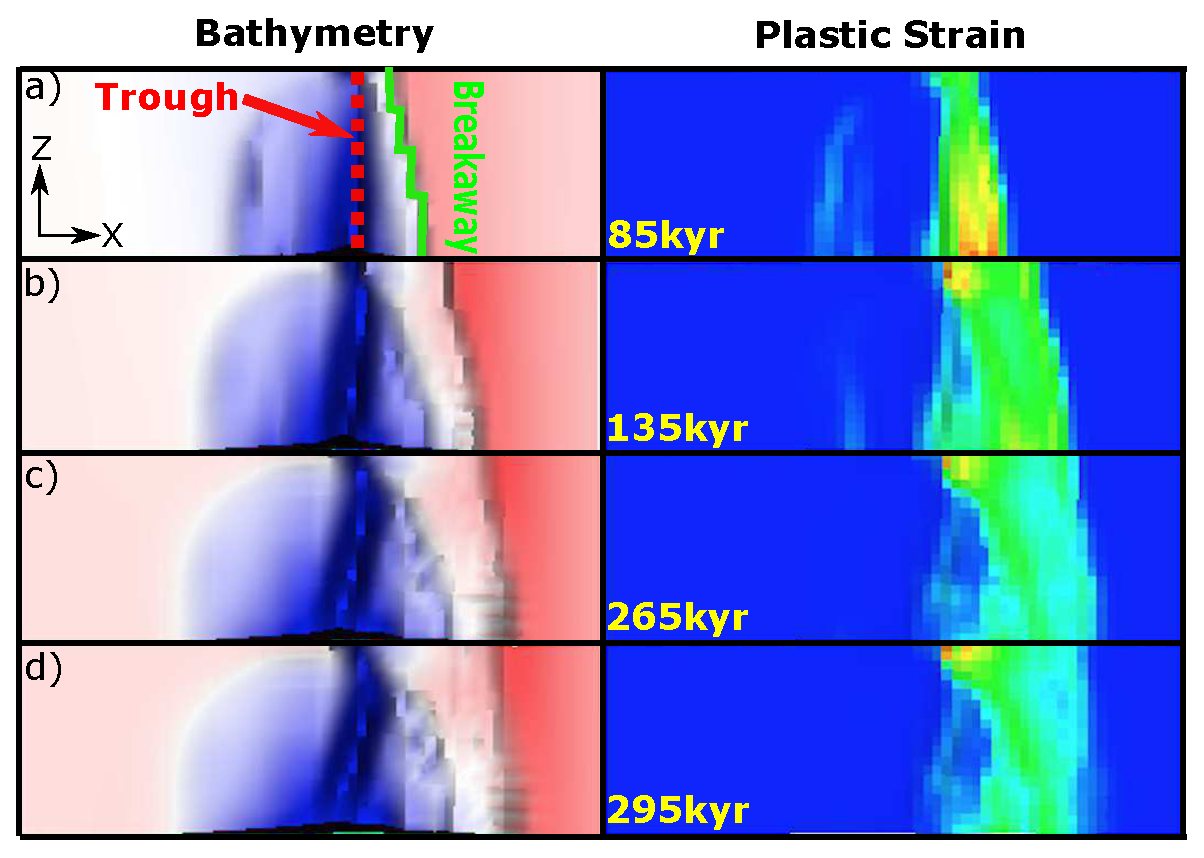
\includegraphics[width=0.6\textwidth]{./Figures/fig_Results1_4.eps}
   \caption[Bird's-eye view of a breakaway in the reference model.]{Bird's-eye view of a breakaway in the reference model at a) 85 kyr, b) 135 kyr, c) 265 kyr and d) 295 kyr. The breakaway is marked by green solid line in a). A narrow zone of depressed topography (``trough'') is marked by red dashed line inside the medain valley (blue area) in a). Color scales are the same with those in Figure~\hyperref[fig_Results1_1]{\ref{fig_Results1_1}}.}
  \label{fig_Results1_4}
\end{figure}

Likewise, the model produces a median valley that widens and deepens with rates inversely proportional to the M value (i.e., rate of local magma supply) (Fig.~\hyperref[fig_Results1_1]{\ref{fig_Results1_1}a-c}; Fig.~\hyperref[fig_Results1_4]{\ref{fig_Results1_4}a-d}).  %OCCs with more than one kilometer in relief and tens of kilometers in wavelentgh are produced. One interesting behavior worth noting is that corrugations with wavelengths of hundred-to-thousand meters and amplitudes of ten-to-hundred meters are also produced.

%The along-ridge coupling forces (i.e. torsion (clockwise); shearing ($\sigma_{xz}$)) prevent relative displacement between the two neighbors along the ridge axis. These along ridge coupling forces on the other hand assist in fault propagation from the lower M side (M = 0.2) to the higher M side (M = 0.8) and reduces the time difference in the initiation of faulting along the ridge axis when comparing with seperated pseudo-2D models.

By 52.5 kyr (Figure~\hyperref[fig_Results1_1]{\ref{fig_Results1_1}.b}), the normal fault on the right-hand side of the ridge axis remains active while the one on the left becomes inactive. The upper part of the active fault plane (shown as plastic strain in the model) is exposed to the seafloor. As the active fault slips, crust at the footwall bends in a clockwise rotation as is illustrated in Figure~\hyperref[fig_Results4_8]{\ref{fig_Results4_8}}. %The neutral plane ($\sigma_{xx}=0$) is shown as the boundary between blue (compression) and pink (tension) (inset of Figure~\hyperref[fig_Results1_1]{\ref{fig_Results1_1}.b}).
%The choice of which fault to survive seems determined by a small numerical perturbation between the two faults seen in Figure~\hyperref[fig_Results1_1]{\ref{fig_Results1_1}.a} although the model setup is symmetrical across the ridge axis. 

%with its front edge extending away from the ridge axis following the spreading plate.
\begin{figure}[h]
   \centering
     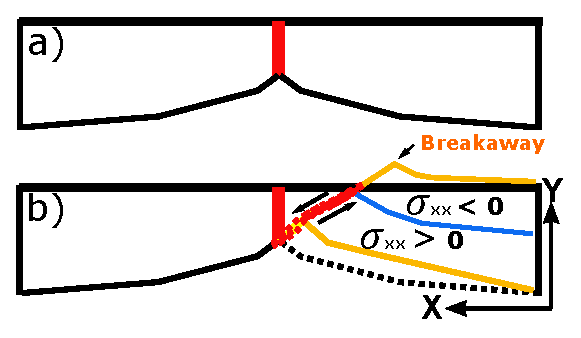
\includegraphics[width=0.6\textwidth]{./Figures/fig_Results4_8_sqrt_cut_back_bending_cartoon.eps}
   \caption[Illustration of bending stresses in lithosphere associated with faulting at the MOR.]{Illustration of the development of bending stress in lithosphere associated with faulting at the MOR. The blue line is the neutral plane where $\sigma_{xx}=0$. Above the neutral plane is compression ($\sigma_{xx}<0$) and beneath it is tension ($\sigma_{xx}>0$).}
  \label{fig_Results4_8}
\end{figure}

%the fault displacement at the front side is larger than that of the back because M is lower at the front and more extension needed to be accommodated by the tectonic processes (i.e. normal faulting). \annote[XT]{Thus, the breakaway at the front extending further away from the ridge axis.}{I am not sure whether the breakaway extends further at lower M side because it should be the same. The breakaway at lower M side does extend further not because of fault slip rate difference but becauses of initiation time, at lower M side, fault begin earlier thus the breakaway begin to extend earlier and reach further, however, the rate of extending away from axis for the breakway should equal to the extension rate $V_{x}$. Thus the offset between breakaways of front and back remains constant} The termination of the detachment fault where footwall begins to be exhumed to the surface will extend further due of faster bending of the footwall at the lower M side. This will also result in a larger volume of exhumation at the lower M side than that of the higher M side. For our model that even when $M=0.2$, the detachment fault can still last for a long time \citep{Baines2008}, the exhumation rate has a upper limit of extension rate of $V_{x}$ in spite of a higher fault slip rate at lower M side.  

%The termination of the detachment fault at the lower M side (M $<$ 0.3) is at $\sim$15km from the ridge axis 
The active normal fault on the right rotates to a lower dip of $\sim$30 $\degree$ at the root of the fault and to $\sim$0 $\degree$ at the exposed fault interface after about 240 kyrs (Fig.~\hyperref[fig_Results1_1]{\ref{fig_Results1_1}.c}). However, the normal fault at the higher M side (especially for M $>$ 0.7) experiences less fault rotation and the termination of the fault is closer to the ridge axis. The maximum relief between the breakaway and the trough inside the median valley becomes larger than 1 km. In addition, $\sim$2 km wavelength corrugations begin to form between the breakaway and termination at the lower M side (M $<$ 0.35). I discuss the formation mechanism for the corrugations in Discussion.
%
%The corrugations show a uniform wavelength which is smaller than that of the mullion structures (Figure~\hyperref[fig_Results1_1]{\ref{fig_Results1_1}.g}). Formation mechanism for these structures are discussed in one of the following sections.  

By 650 kyr (Figure~\hyperref[fig_Results1_1]{\ref{fig_Results1_1}.d}), the detachment fault reaches its lowest dip angle and its termination stops moving away from the ridge axis. The original breakaway of this detachment has already moved out of the model domain.
%\annote[XT]{moved out of the model domain}{it should not, if breakaway move with 25km/yr(half spreading rate), since the distance between initial break (5km away from ridge center) and right wall of the model domain is about 25km which needs 1Myr to reach. But now is only 650 kyr. Why is it?}.
The total fault offset at this point is greater than the thickness of the crust and thus would be sufficient for exhuming the upper mantle materials. %The previous fault interface bends over and dips away from the ridge axis, producing a cylindrical OCC. 
%A hint of the inward fault jump appears up over the area corresponding to 0.5 $<$ M $<$ 0.65.
%\add[XT]{Its formation will be discussed in Discussion section accompanied by the stress status analysis. }

A new near-axis fault first appears at the center of the model domain with M $\in$ (0.5, 0.65) and then propagates in positive $z$ direction (Fig.~\hyperref[fig_Results1_1]{\ref{fig_Results1_1}.d,e}). At this time, the initial detachment fault is still active and takes up most of the extension. %The distance between the termination of the detachment fault and the ridge axis is shorter at the higher M side because the detachment fault at the higher M side remains in a relatively higher dip angle due to less fault slip and thus less bending in the footwall. This along ridge variation in the location of termination produces a mullion structure with a wavelength of $\sim$6 km and an amplitude of several hundred meters. Two smaller scale mullions are also identified on the surface of the larger one (Fig.~\hyperref[fig_Results1_1]{\ref{fig_Results1_1}.g}).

The new near-axis normal fault at the higher M side cuts through the hanging wall of the detachment fault at 880 kyr (Fig.~\hyperref[fig_Results1_1]{\ref{fig_Results1_1}.f}). It coexists with the initial detachment fault and begins to accommodate most of the intra-plate extension. This event is called the ``inward fault jump'' [\citealp{Tucholke1998}; \citealp{Dick2008}].  %However, it still coexists with the initial detachment fault (shown in the inset). 

By 910 kyr (Fig.~\hyperref[fig_Results1_1]{\ref{fig_Results1_1}.g}), the inward fault jump completes in the M $> 0.5$ region: the new high-angle fault takes up all the extension and the initial detachment fault becomes completely inactive. The block that was previously a hanging wall to the detachment becomes a footwall of the new fault, passively moving with the plate to the negative $x$-axis direction. At the lower M side, the detachment is still active and the hanging wall continues to move toward the positive $x$-axis direction (Figure~\hyperref[fig_Results_1_velocity_field]{\ref{fig_Results_1_velocity_field}}). This dextral sense of relative motions between the high and the low M side produces a region of sinistral shear stress $\sigma_{xz}$ (Figure~\hyperref[fig_Results_1_Sxz]{\ref{fig_Results_1_Sxz}}) and eventually creates a transfer fault (Fig.~\hyperref[fig_Results1_1]{\ref{fig_Results1_1}.h}). %at the lower M side (M $<$ 0.5) $\sim$45 $\degree$ oblique to the ridge axis (Figure~\hyperref[fig_Results_1_Sxz]{\ref{fig_Results_1_Sxz}}) and the shear stress zone produces a new trough inside the median valley that aligns with it. Combined with the previous trough, an ``X'' shape topography low is created in the model.
As the inward jumped fault evolves, another dome ajacent to the initial OCC is produced at the higher M side by 1000 kyr.% (Fig.~\hyperref[fig_Results1_1]{\ref{fig_Results1_1}.h}).  

\begin{figure}[h]
  \centering
    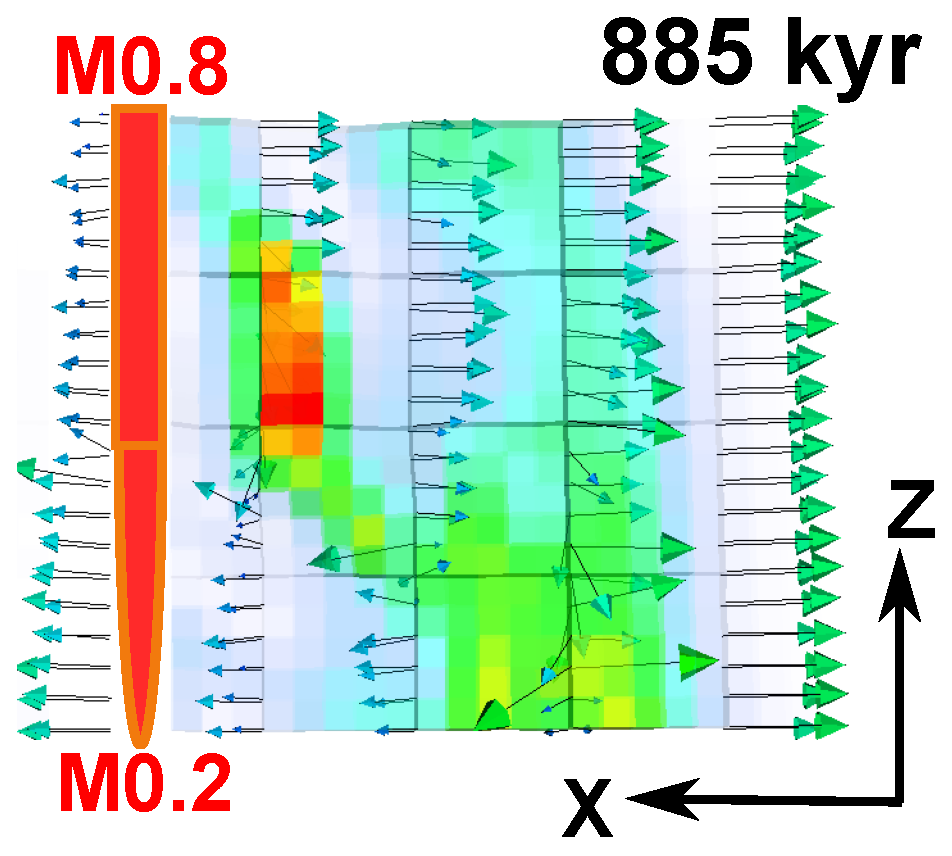
\includegraphics[width=0.5\textwidth]{./Figures/fig_Results_1_velocity_field.eps}
  \caption[Bird's-eye view of velocity field with plastic strain ploted with opacity linearly proportional to its value.]{Bird's-eye view of velocity field with plastic strain ploted with opacity linearly proportional to its value. (color scale is the same as Figure~\hyperref[fig_Results1_1]{\ref{fig_Results1_1}.a)})}
 \label{fig_Results_1_velocity_field}
\end{figure}

\begin{figure}[h]
   \centering
     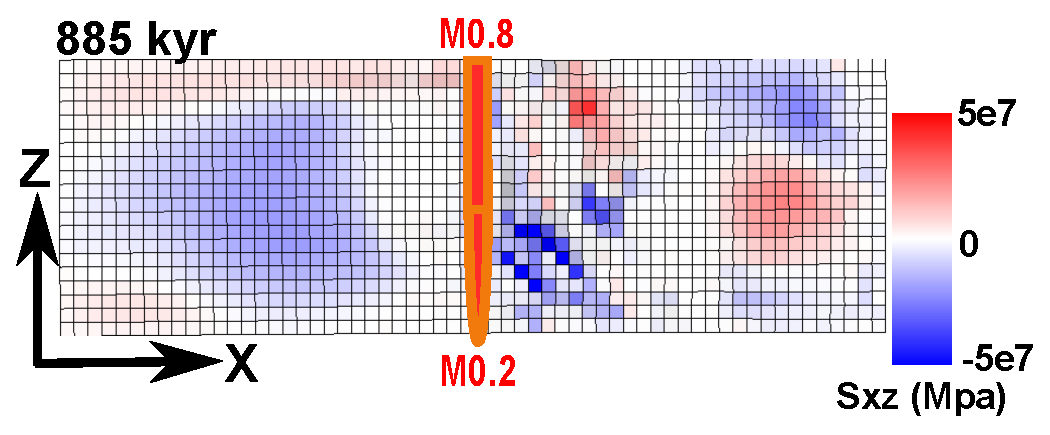
\includegraphics[width=0.8\textwidth]{./Figures/fig_Results_1_Sxz.eps}
   \caption{Bird's-eye view of $\sigma_{xz}$.}
  \label{fig_Results_1_Sxz}
\end{figure}

% %Initially, the edge of fault interface that is moving with the footwall corresponds to the right boundary of the plastic strain. 
% Among other noticeable behaviors of the reference model are the time-dependent change in the geometry of the detachement fault's breakaway and the trough within the median valley. The along-ridge offset of the breakaway is initially established according to the variation in M but reduces at $\sim$295 kyr (Figure~\hyperref[fig_Results1_4]{\ref{fig_Results1_4}.d}) making the breakaway subparallel with the ridge axis. Several factors contribute to this morphological transision. The long-lived normal fault at the lower M side reaches and stays at its minimum dip angle at around 240 kyr (Figure~\hyperref[fig_Results1_4]{\ref{fig_Results1_4}.c}).
% %its termination stops moving further away from the ridge axis and 

%The healing effect implemented in this model \citep[e.g.,][]{Tucholke2008} reduces plastic strain (thereby restores cohesion) of the non-slipping portion of the fault interface that has been exhumed to the seafloor. At the higher M side, the termination keeps moving away from the ridge axis. This reduces the initial offset generated by the asynchronous initiation of faulting. 
% In contrast, the trough is initially straight and parallel to the ridge axis (Figure~\hyperref[fig_Results1_4]{\ref{fig_Results1_4}.a}) but becomes oblique to the ridge axis. The obliquity increases with the amount of extension (Figure~\hyperref[fig_Results1_4]{\ref{fig_Results1_4}.b$\sim$d}). This change in the trough geometry is due to 


%\iffalse    
\subsubsection{Constant M model M88ConT2}
%\add[XT]{I still prefer to have M88ConT2 because: 1.As a comparison to the varing M model, it help to show the importance of M variation(corrugation, mullion, median valley variation, inward fault jump etc. 2. it itself is a mode of MORs topography formation mechanism, those higher frequency symmetrical abyssal hills.} \add[EC]{Sorry, but I don't agree. This section can be simply summarized as, ``a constant M shows similar behaviors with a corresponding 2D model from the previous studies and (obviously) does not show along-ridge variations in terms of morphology and faulting''. If you really want, say something like this upfront, like, where you first introduce the reference model.}

As a comparison to the varying M models, a constant M model is run. It shows similar behaviors with corresponding 2D models from the previous studies and does not show along-ridge variations in terms of morphology and faulting.

As shown in Figure~\hyperref[fig_Results1_3]{\ref{fig_Results1_3}}, model M88ConT2 produces a $\sim$20 km wide and 1$\sim$2 km deep median valley, which is similar to the observation of the Mid-Atlantic Ridge. The width and depth of the median valley is almost constant along the ridge as contrast to the varying M models. The variation of the location of the breakaway and termination along the ridge that is mentioned in the reference model (M28LinT1) does not show up. Because the magma supply is constant along the ridge with M = 0.8, there is no stress perturbation along the ridge. Thus, the normal faults along the ridge initiate at the same time and the slipping rate of the fault is also constant along the ridge axis. The synchronized fault initiation results in no offset between breakaways and the constant sliping rate produces no along ridge axis variation in the position of the termination. In addition, neither corrugations nor mullion structures are generated. Normal faults alternate on each side of the ridge axis with a period of $\sim$10 km of plates extension and produce symmetrical shorter wavelength abyssal hills.

\begin{figure}[h]
  \centering
    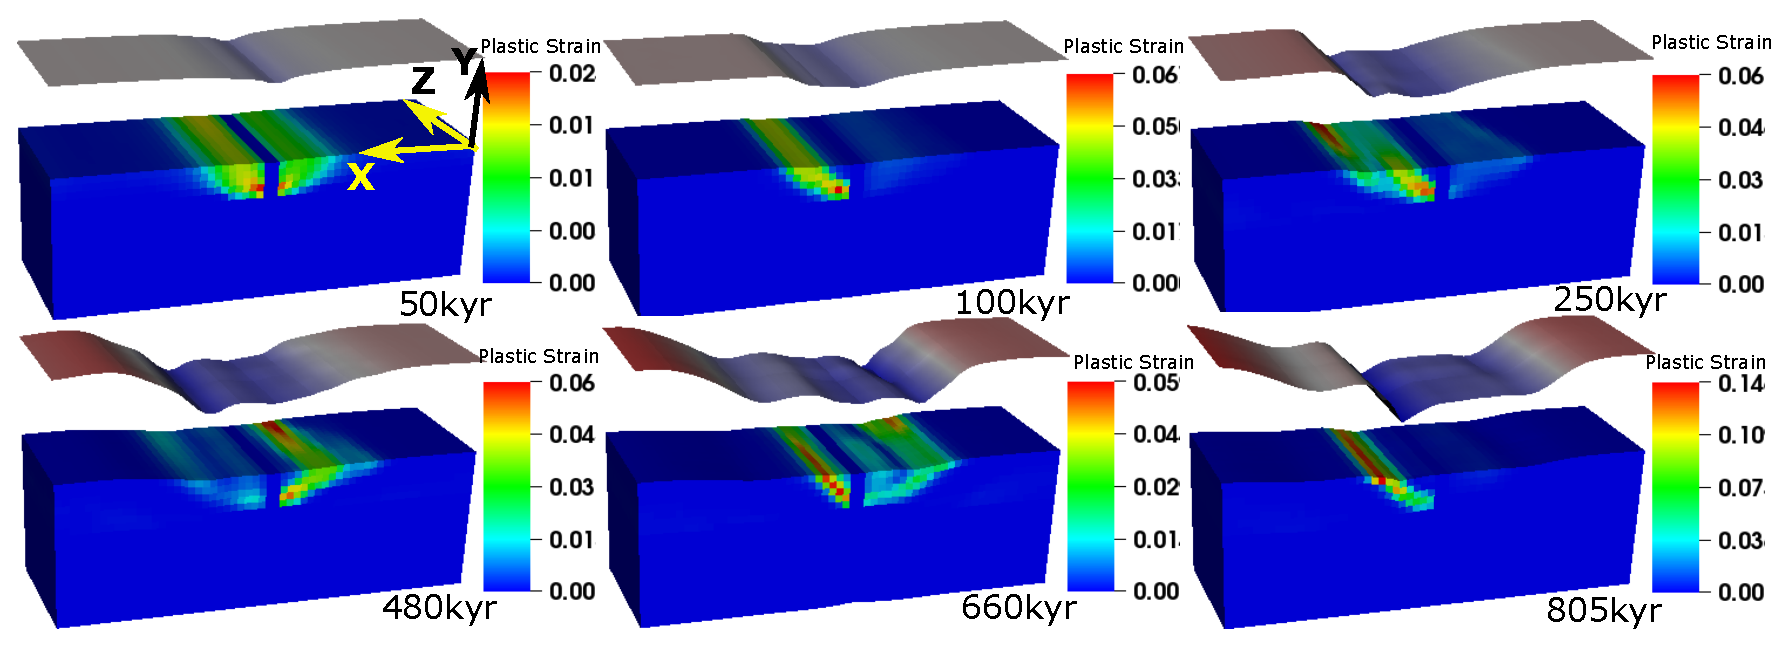
\includegraphics[width=1.0\textwidth]{./Figures/fig_Results1_3.eps}
  \caption{Evolution of plastic strain and surface topography of the model: M88ConT2 (Table~\hyperref[Tab1_1]{\ref{Tab1_1}}). Color scale of topography is the same as Figure~\hyperref[fig_Results1_1]{\ref{fig_Results1_1}.a}.}
 \label{fig_Results1_3}
\end{figure}   

%For 3D models, why and how fault alternates on each side of the ridge axis is different from the previous 2D studies and is described in the following sections. \add[XT]{Three analysis and equations for fault alternation need to bederived. three components 1) resisting bending force 2) resisting gravity work and 3) assisting weakening} 
%\fi

\subsection{Main structural characteristics}
I describe seven structural characteristics of the models: location of the termination, geometry of the trough, inward fault jump, fault alternation, mass wasting, hourglass-shaped median valley and corrugations and mullion structures. Since the details of these features differ among the models, they are useful for delineating and contrasting complicated model behaviors.

\subsubsection{Location of termination}
\iffalse
\add[XT]{for the term ``termination'' please refer to:}
23 times usage from \citep{Canales2008} or
 \citep{Blackman2009} or
 figure one of \citep{Dick2008} or
 figure six of \citep{Mallows2012} or
 figure 1,2,3A of \citep{Schouten2010} 
But \citep{Reston2011a} give a further discussion on it and they favor ``top hanging wall cutoff''.
they also mention that ``The traditional map term fault trace, which is not generally used on sections, is not appropriate as it cannot be used to describe the geometry of a structure everywhere buried by later sedimentary rock.''
\fi

Location of a fault termination varies along the ridge as indicated by black dashed lines in Figure~\hyperref[fig_Results1_1]{\ref{fig_Results1_1}} and black arrows in Figure~\hyperref[fig_Results1_2]{\ref{fig_Results1_2}}. The highest strain rate regions (red) in Figure~\hyperref[fig_Results1_2]{\ref{fig_Results1_2}} can be interpreted as the active detachment fault interfaces. Compared to the two slices with M $>$ 0.5, the distances between terminations and the ridge axis at the lower M side (M $<=$ 0.5) is larger and the dip angles of the detachment faults are lower. For the ridge region with M $>$ 0.5, the fault root is pushed away from the ridge axis due to excessive diking while the termination is closer to the ridge axis due to lower slipping rate of the fault and the asynchronous initiation of faulting along the ridge. Thus the distance between the termination and the fault root is smaller at the higher M side and the dip angle of the fault is higher. However, among the three slices of M $<=$ 0.5, the distances and the dip angles are similar. This is because one end of the detachment fault roots at the same places along the ridge axis (intersection between the center dike and the brittle-ductile transition), and for the other end, the moving rate of the termination has a maximum value that is restricted by the far field extension rate $V_{x}$. Thus, the bending rates of the detachment faults are similar among the three slices of M $<=$ 0.5.

\begin{figure}[h]
  \centering
    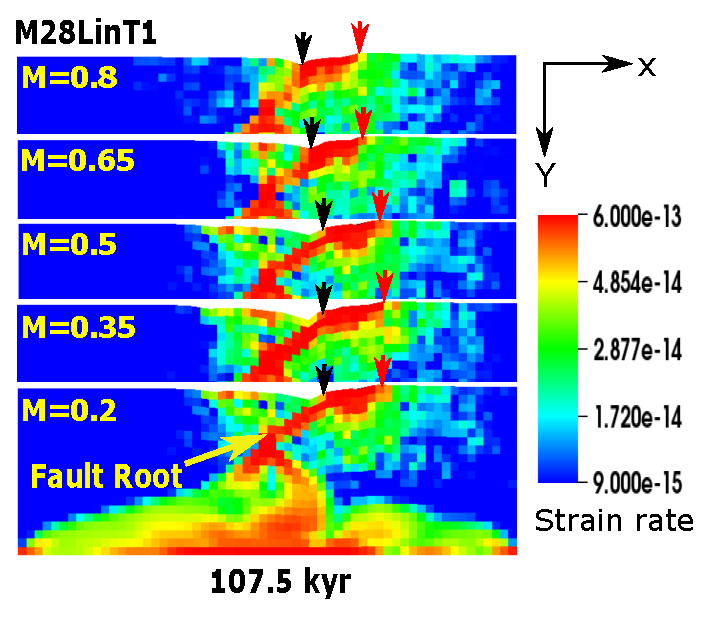
\includegraphics[width=0.6\textwidth]{./Figures/fig_Results1_2.eps}
  \caption[The second invariant of strain rates plotted on the reference model's vertical cross sections along the ridge at 107.5 kyr.]{The second invariant of strain rates plotted on the reference model's vertical cross sections along the ridge at 107.5 kyr. Terminations and breakaways are marked by black and red arrows.}
 \label{fig_Results1_2}
\end{figure}   

%In other words, in order to spend least frictional energy during faulting, the detachment fault interface between the two ends (termination and fault root) tends to be a straight line.     Thus, the dip angle of the detachment fault is inversely proportional to the distance between the termination and the root of the fault when M $<$ 0.5. Since the breakaways at the lower M side (M $<$ 0.5) moves with the extending plate under the same velocity $V_{x}$, and the initiation time difference of the normal faults at the lower M side is similar (Figure~\hyperref[fig_Results1_1]{\ref{fig_Results1_1}.a}), the distances between the breakaways and the roots of the faults are the same. Meanwhile, the distance between breakaways and terminations as indicated by the red and black arrows in the Figure~\hyperref[fig_Results1_2]{\ref{fig_Results1_2}} is similar along the ridge axis. Thus the dip angles of the faults at the same time along the ridge-axis are very much the same. However, when M $>$ 0.5 (Figure~\hyperref[fig_Results1_2]{\ref{fig_Results1_2}, (M = 0.65, 0.8)}), the amount of fault slip decreases as M increases. The crust at the footwall experiences less bending and the detachment fault remains in a higher angle as well as that the terminations are closer to the ridge axis. Because the root of the fault is slowly pushed away from ridge axis while the breakaways of the faults are closer to ridge axis due to a later initiation of the fault. In addition, the crust thickness that the fault cuts through is slowly increasing as the fault being pushed away from ridge center due to excessive diking. These three factors together contribute to a higher dip angle. In a unit time, the volume of the exhumation is also smaller for the higher M side.

%Location of a fault termination varies along the ridge as indicated by black dashed lines in Figure~\hyperref[fig_Results1_1]{\ref{fig_Results1_1}} and black arrows in Figure~\hyperref[fig_Results1_2]{\ref{fig_Results1_2}}). The highest strain rate regions (red) shown in Figure~\hyperref[fig_Results1_2]{\ref{fig_Results1_2}} can be interpreted as the active detachment fault interfaces. 
%The reference model shows that the distance from the ridge axis to the termination of the detachemtn fault is greater on the lower M side than on the higher M side because faulting starts at the lower M side and initiates later on the higher M side. %Because the distance between the termination and the fault root is smaller at the higher M side, the dip angle of the fault is higher.
%The distance between the termination and the ridge axis as well as the dip angle of the buried portion of the detachment do not show correlation with M values when M $<$ 0.5. %Because the rotation rate of the detachment fault is determined by how fast the termination move away from the fault root. 
%Since the detachment faults for the ridge region of M $<$ 0.5 root at the same place at the intersection between the center dike and the brittle-ductile transition (BDT) and the moving rate of the termination has a maximum value that is restricted by the far field extension rate $V_{x}$, the distances between the terminations and fault roots of the detachment faults is similar among the three slices of M $<=$ 0.5. In addition, in order to spend least frictional energy during faulting, the detachment fault interface between the two ends (termination and fault root) tends to be a straight line. Thus, the dip angle of the detachment fault is inversely proportional to the distance between the termination and the root of the fault when M $<$ 0.5. Since the termination at the lower M side (M $<$ 0.5) moves with the spreading plate with same velocity $V_{x}$, and the initiation time difference of the normal faults at the lower M side is similar (Figure~\hyperref[fig_Results1_1]{\ref{fig_Results1_1}.a}), the distances between the terminations and the roots of the faults are the same. %Meanwhile, the distance between breakaways and terminations as indicated by the red and black arrows in the Figure~\hyperref[fig_Results1_2]{\ref{fig_Results1_2}} is similar along the ridge axis.
%Thus the dip angles as well as the distance between the termination and the ridge axis of the faults at the lower M side are similar. 
%In contrast, when M $>$ 0.5, the distance from the ridge axis to the termination decreases with increasing M (Figure~\hyperref[fig_Results1_2]{\ref{fig_Results1_2}}). The crust at the footwall experiences less bending and the detachment fault remains in a higher angle as well as that the terminations are closer to the ridge axis. Because the root of the fault is slowly pushed away from ridge axis while the termination of the faults are closer to ridge axis due to a later initiation of the fault. ,  %In addition, the crust thickness that the fault cuts through is slowly increasing as the fault being pushed away from ridge center due to excessive diking. These three factors together contribute to a higher dip angle. In a unit time, the volume of the exhumation is also smaller for the higher M side.

One thing needs to be noted is that the trough at the higher M side corresponds to the terminations but detached from the terminations at the low M side (M $<$ 0.5) as shown in Figure~\hyperref[fig_Results1_2]{\ref{fig_Results1_2}}.

\subsubsection{Geometry of trough}

The depressed narrow region that developes in the median valley is termed ``trough''. The reference model showed that its shape in the bird's eye view evolves from a straight line parallel to the ridge axis to a line oblique to the ridge axis (Figure~\hyperref[fig_Results1_4]{\ref{fig_Results1_4}.a-d}). Initially, the trough along the ridge corresponds to the termination. However, at the lower M side (M $<$ 0.5), as the normal fault rotates to a lower dip, the trough is no longer coincident with the fault termination and is moving slowly to the left because the hanging wall is pulled by the conjugate plate. %Also, the trough at the lower M side is pulled to the conjugate plate to the negative $x$-axis direction. 
However, the trough on the higher M side (M $>$ 0.5) is pushed away from the ridge axis \citep{Tucholke2008}. But since the trough cannot bypass the termination, the trough at M = 0.8 is restricted closer to the ridge axis. Together it generates the curved shape of the trough (Figure~\hyperref[fig_Results1_4]{\ref{fig_Results1_4}.d}). 
%{Important tecnique from discussion on Mar. 9th with Eunseo: 1. One way to analyze models is to make hypothesis to describe model behaviors and than use models to approve or reject it. If rejected, find a new hypothesis and do the same thing again.}
%\add[XT]{4. An new thinking on little termination or dip angle variation when M$<0.5$ as observed in %figure~\ref{fig_Results1_2}: why along-z hanging wall has little variation is because we have along z coupling, the rotational shear failure between along-z neighbors are so hard. and also, the more extension in M0.2 end is accommodated elastically by the whole plate to the left of the detachment fault which can be observed as lower topo(topography variation along ridge axis).} 
%\add[XT]{One question needs to be answered: at 410 timesteps (205kyr), the breakaway at the front already extends 15km. If assumming a constant extending rate, it means a velocity of around 75km/Myr, much faster than half spreading rate 25km/Myr. If it is true, I need to change previous discussion on how fast breakaway being pulled away from ridge-axis.}


\subsubsection{Inward fault jump}

The inward fault jump (e.g., Fig.~\hyperref[fig_Results1_1]{\ref{fig_Results1_1}.f}) occurs in most of the models when the energy for maintaining an old fault becomes larger than breaking a new one near the ridge axis. As shown in Figure~\hyperref[fig_Results1_2]{\ref{fig_Results1_2}}, at the region with M $>$ 0.5, the existing normal fault is pushed away from the ridge-axis due to robust diking (M $>$ 0.5). As it moves away from the ridge axis, the frictional energy for the fault, the bending energy for the footwall as well as the negative work done by gravity that resists the exhumation of the footwall increase [\citealp{Lavier2000, Olive2014}]. The initial detachment fault remains active until the sum of the negative works reaches an upper limit that breaking a new fault near the ridge axis needs less work than to maintain the initial one, the initial detachment fault at the higher M side is then substituted by the inward jumping fault that cuts through the previous hanging wall. As the fault evolves, it connects to the initial detachment at the lower M side (M $<$ 0.5) by a transfer fault and generates a curved termination along the ridge. Unlike fault alternation described below, the inward fault jump occurs on the same side of the ridge axis with its along-axis extent corresponding to the M $>$ 0.5 region.
%, at the region with M $>$ 0.5, the existing normal fault is pushed away from the ridge-axis due to \annote[EC]{excessive}{Doesn't sound appropriate. Probably you mean, ``frequent''.} diking (Figure~\hyperref[fig_Results1_1]{\ref{fig_Results1_1}.c,d}). As it moves away from the ridge axis, the \annote[EC]{frictional energy}{What do you mean?} for the fault, the bending energy for the footwall as well as the \annote[EC]{negative}{What do you mean?} work done by gravity that resists the exhumation of the footwall increase [\citealp{Lavier2000, Olive2014}]. The initial detachment fault remains active until the negative works reach an upper limit that breaking a new fault near the ridge axis needs less work than to maintain the initial one, the initial detachment fault at the higher M side is substituted by the inward jumping fault that cuts through the previous hanging wall. This inward jumping behavior of the normal fault is termed as ``inward fault jump''.
%\add[XT]{for the description of the previous commented out paragraphy, please refer to:}[\citealp{Lavier2000}; \citealp{Olive2014}]

%The new fault usually forms on the high M side first and it connects to the existing detachment developing on the lower M side (M $<$ 0.5), producing a curved fault termination. Unlike fault alternation described below, the inward fault jump occurs on the same side of the ridge axis with its along-axis extent corresponds to the M $>$ 0.5 region. %rather than cut through the whole MOR segment.

\subsubsection{Fault alternation}

Fault alternation is the behavior that normal faults alternatively show up on each side of the ridge axis when magma supply is robust enough, as shown in M88ConT2 (Figure~\hyperref[fig_Results1_3]{\ref{fig_Results1_3}}). The normal fault first evolves on the left-hand side of the ridge axis and produces an abyssal hill parallel to the ridge axis. By 480 kyr, another normal fault evolves on the other side of the ridge axis and replaces the first one. Note that among the 15 models (Table~\hyperref[Tab1_1]{\ref{Tab1_1}}), only three produce fault alternation. They are M88ConT2, M58SinT2 and M58SqrtT2. Fault alternates only when weakening rate is low (type 2 weakening) and the average integration of M along the ridge is larger than 0.65. Analysis on when and why fault alternates is given in the Discussion section.

%When M is high enough, a normal fault first forms on one side of the ridge axis but another fault forms on the other side when the first one locks (Fig.~\hyperref[fig_Results1_3]{\ref{fig_Results1_3}}) \citep{Buck2005,Tucholke2008}. This behavior is termed as ``fault alternation''. %Among the 12 models (Table~\hyperref[Tab1_1]{\ref{Tab1_1}}), only three models produces fault alternation. They are M88ConT2, M58SinT2 and M58SqrtT2. Fault alternates only when weakening rate is low (type 2 weakening) and the average integration of M along the ridge is larger than 0.65. Analysis on when and why fault alternates is given in ``Discussion'' section.

\subsubsection{Mass wasting}\label{para_CutBack}

%\add[XT]{For ``shear-wasting'', shear is from the three triggering shear stresses, wasting is from mass wasting. For mass wasting, it has the benefit that people are familiar with this term, however, the new mechanism for triggering it(the shear stress) is missing}\note[EC]{Didn't we agree that shear stress seen in the vertical cross-section does not trigger this event?}

Mass wasting occurs on the exposed surface of a low-angle normal fault. When the weak fault zone becomes gravitationally unstable and is decoupled from the spreading plate as well as the underlying material, the detached layer flows towards the lower ridge axis and the lower M side driven by gravity with a velocity hundreds of times faster than the half spreading rate (Figure~\hyperref[fig_Results_3_2_5_Cut-back_velocity]{\ref{fig_Results_3_2_5_Cut-back_velocity}}; Figure~\hyperref[fig_Results4_4]{\ref{fig_Results4_4}.b,e (first row)})). As the top layer of the hanging wall flows down the topography slope, obvious topography drop is observed in 2.5 kyr (Figure~\hyperref[fig_Results4_4]{\ref{fig_Results4_4}.b) versus c); d) versus e) (topography)}).

\begin{figure}[h]
  \centering
    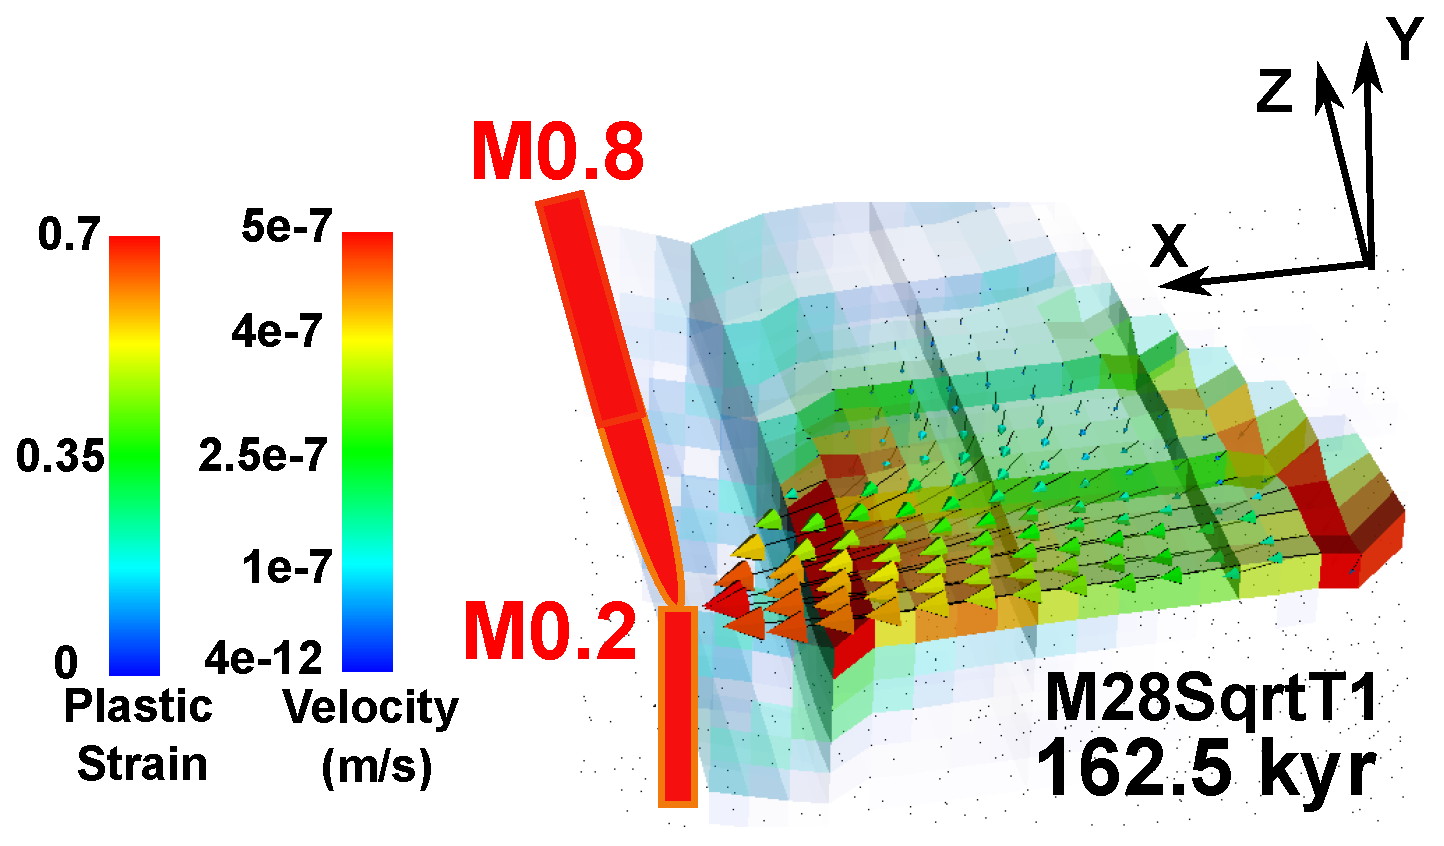
\includegraphics[width=0.6\textwidth]{./Figures/fig_Results_3_2_5_Cut-back_velocity.eps}
  \caption[Velocity of the mass wasting hanging wall.]{Velocity of the mass wasting hanging wall. Magnitudes of the velocity are shown by the colors of the arrow heads. Plastic strain is plotted with opacity linearly proportional to its value.}
 \label{fig_Results_3_2_5_Cut-back_velocity}
\end{figure}   

Mass wasting is triggered by several factors. First, when the tip of the weak fault interface moves away from the ridge axis with the spreading plate and is intersected by a pre-exisitng shear stress $\sigma_{xy}$ (Figure~\hyperref[fig_Results4_5]{\ref{fig_Results4_5}}), the extra shear stress cuts the tip of the weak fault interface and leads to the decoupling between the breakaway and the upper layer of the hanging wall of the detachment fault. Second, during the roll over of the hanging wall at the breakaway, tensional stress ($\sigma_{xx} >$ 0) promotes the deviatoric stress for generating small scale high angle normal faults cutting the detachment fault surface \citep{Tucholke1998} (Figure~\hyperref[fig_Discussion_Observation_1_Tucholke1998]{\ref{fig_Discussion_Observation_1_Tucholke1998}.c,d}) and in this case the tip of the weak layer. In addition, along ridge coupling tends to resist the increase in along ridge offset of breakway which is generated by along ridge varying slip rates of the faults. As Figure~\hyperref[fig_Results_3_2_5_sqrt_cut_back_Sxz_beneath]{\ref{fig_Results_3_2_5_sqrt_cut_back_Sxz_beneath}} shows, the dextral sense shear stresses (red $\sigma_{xz}$) beneath the top weak layer tends to rotate the upper layer and assists in triggering the decoupling process.  

\begin{figure}[h]
  \centering
    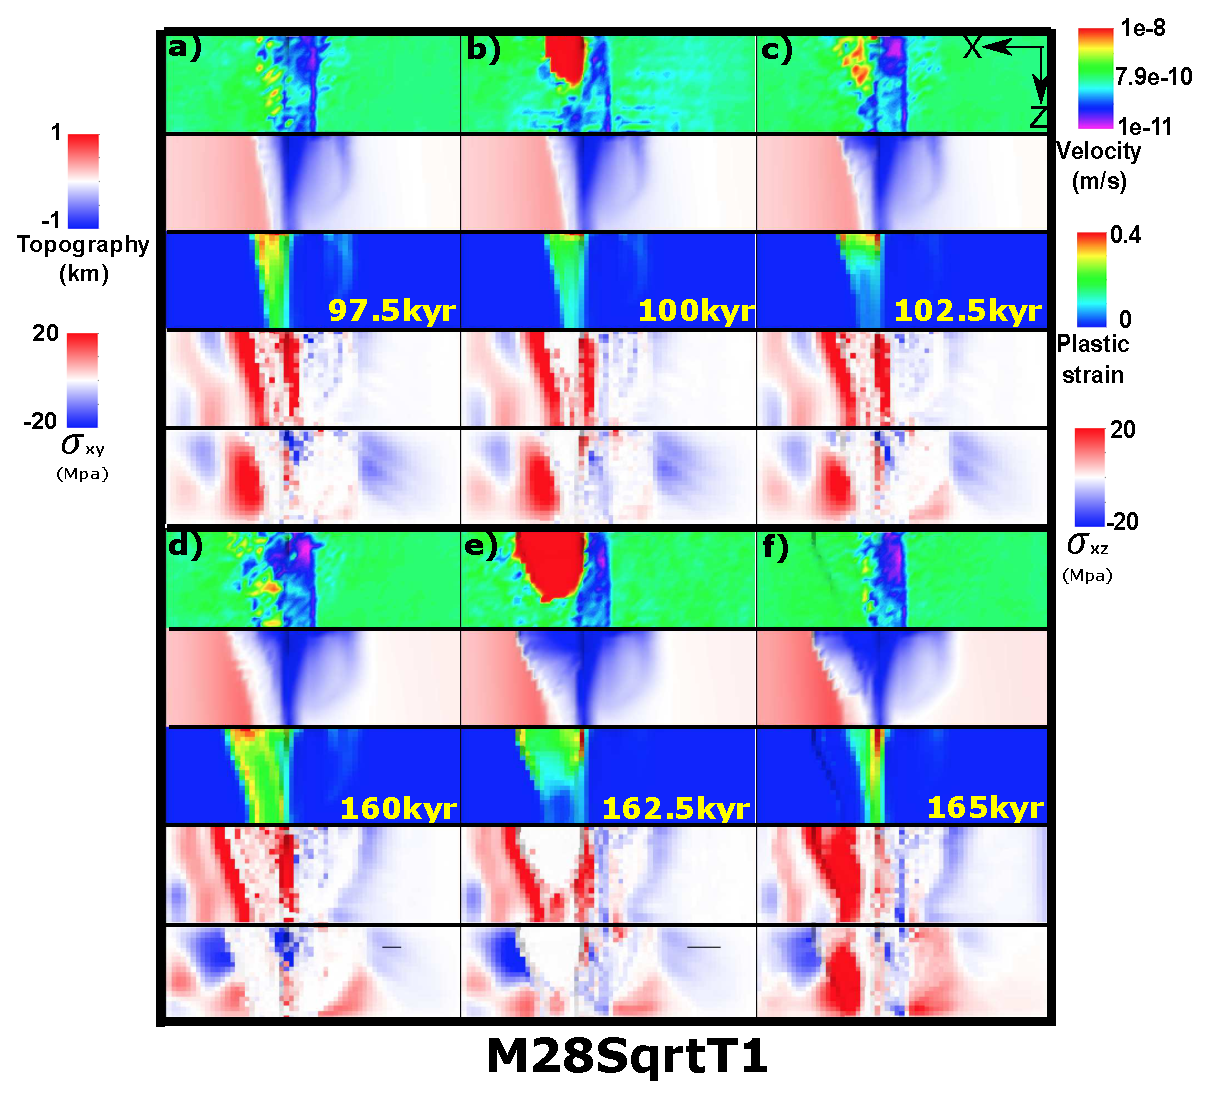
\includegraphics[width=0.8\textwidth]{./Figures/fig_Results4_4_sqrt_cut_back_with_time_1.eps}
  \caption{Plastic strain, topography and stresses evolution for M28SqrtT1.}
 \label{fig_Results4_4}
\end{figure}  

\begin{figure}[h]
  \centering
    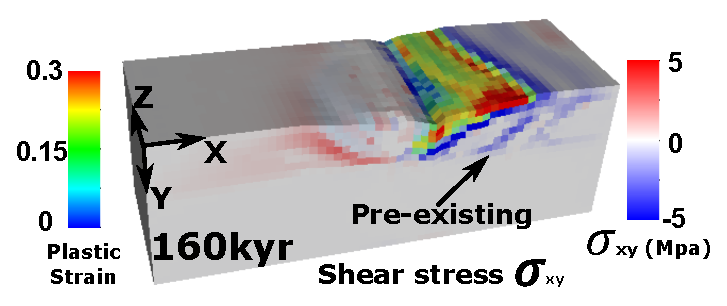
\includegraphics[width=0.6\textwidth]{./Figures/fig_Results4_5_sqrt_cut_back_pre_accummulated_shear_zone.eps}
  \caption[The weak detachment fault tip reaches the pre-existing shear stress.]{The weak detachment fault tip reaches the pre-existing shear stress. Plastic strain is plotted with opacity linearly proportional to its value.}
 \label{fig_Results4_5}
\end{figure}   

\begin{figure}[h]
  \centering
    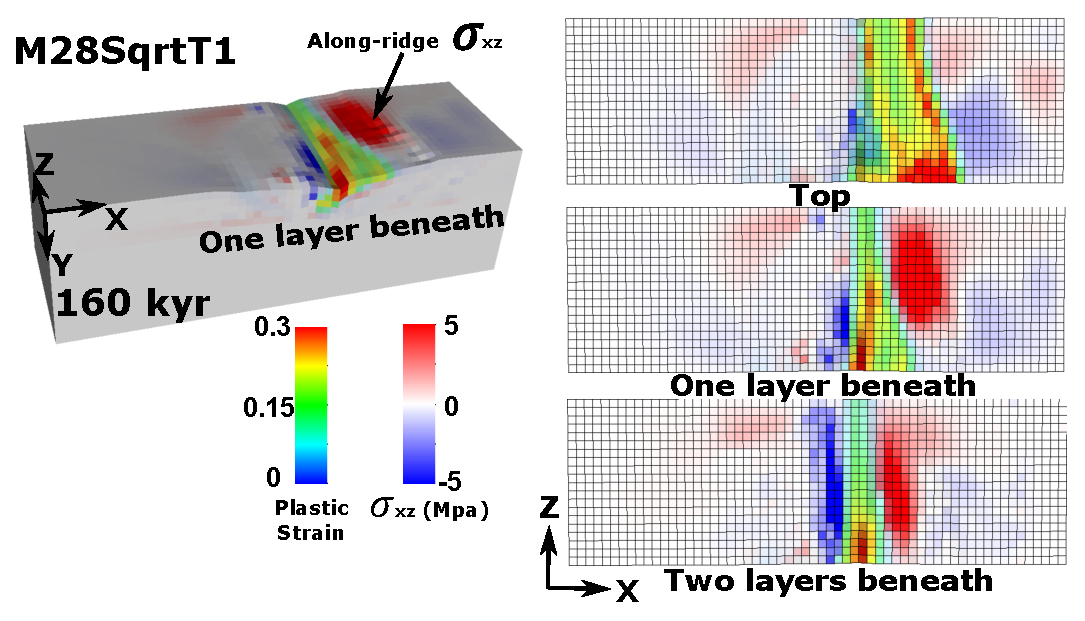
\includegraphics[width=1.0\textwidth]{./Figures/fig_Results_3_2_5_sqrt_cut_back_Sxz_beneath.eps}
  \caption[Along ridge axis $\sigma_{xz}$.]{Along ridge axis $\sigma_{xz}$ (bird's-eye view of three layers of model domain) (positive(red) means clockwise). Plastic strain is plotted with opacity linearly proportional to its value.}
 \label{fig_Results_3_2_5_sqrt_cut_back_Sxz_beneath}
\end{figure}

%The decoupled upper layer of the hanging wall at the higher M side (0.12 $<$ M $<$ 0.56) flows toward the lower M side with a velocity approximately parallel to the ridge axis (Figure~\hyperref[fig_Results_3_2_5_Cut-back_velocity]{\ref{fig_Results_3_2_5_Cut-back_velocity}}). This is because the topography of the median valley at the higher M side is higher due to a larger amount of magma supply. As the top layer of the footwall flows down the topography slope, obvious topography drop is observed in 2.5 kyr (Figure~\hyperref[fig_Results4_4]{\ref{fig_Results4_4}.b) versus c); d) versus e) (topography)}). 

%The mass wasting produces a continuous fault scarp with a relief of $\sim$1 km along the initial breakaway. 
%The total length of the fault scarp extends for about 20 km along the ridge. The distance between the fault scarp and the central dike varies along the ridge (Figure~\hyperref[fig_Results4_4]{\ref{fig_Results4_4}.e (topography)}).




%Five factors together trigger the cut-back. The unbending force of the bent footwall (Figure~\hyperref[fig_Results4_8]{\ref{fig_Results4_8}}); the pre-existing shear stress that add extra cutting force to the extending tip of the weak detachment fault (Figure~\hyperref[fig_Results4_5]{\ref{fig_Results4_5}}); the shear stress that aligns beneath the detachment fault interface that tends to rotate counterclockwise the hanging wall (viewing into positive $z$-axis direction) (Figure~\hyperref[fig_Results4_5]{\ref{fig_Results4_5}}); the coupling between the conjugate plate and the hanging wall at the lower M side (M $<$ 0.5) that pulls the hanging wall toward the ridge axis; and the asynchronous fault inistiation as well as the along ridge variation in the rate of fault slip due to varying M that tend to syncrhonize the faulting along the ridge and resists the faster extension of the termination at the higher M side (Figure~\hyperref[fig_Results_3_2_5_sqrt_cut_back_Sxz_beneath]{\ref{fig_Results_3_2_5_sqrt_cut_back_Sxz_beneath}}).

%As shown in Figure~\hyperref[fig_Results4_8]{\ref{fig_Results4_8}}, due to bending of the crust at the footwall side, below the blue neutral plane, $\sigma_{xx}>0$, meaning tensional stress increases as fault slips. The resulting force tends to unbend the bent crust and drag down the connecting surface (the future decoupled hanging wall).

\iffalse
\begin{figure}[h]
  \centering
    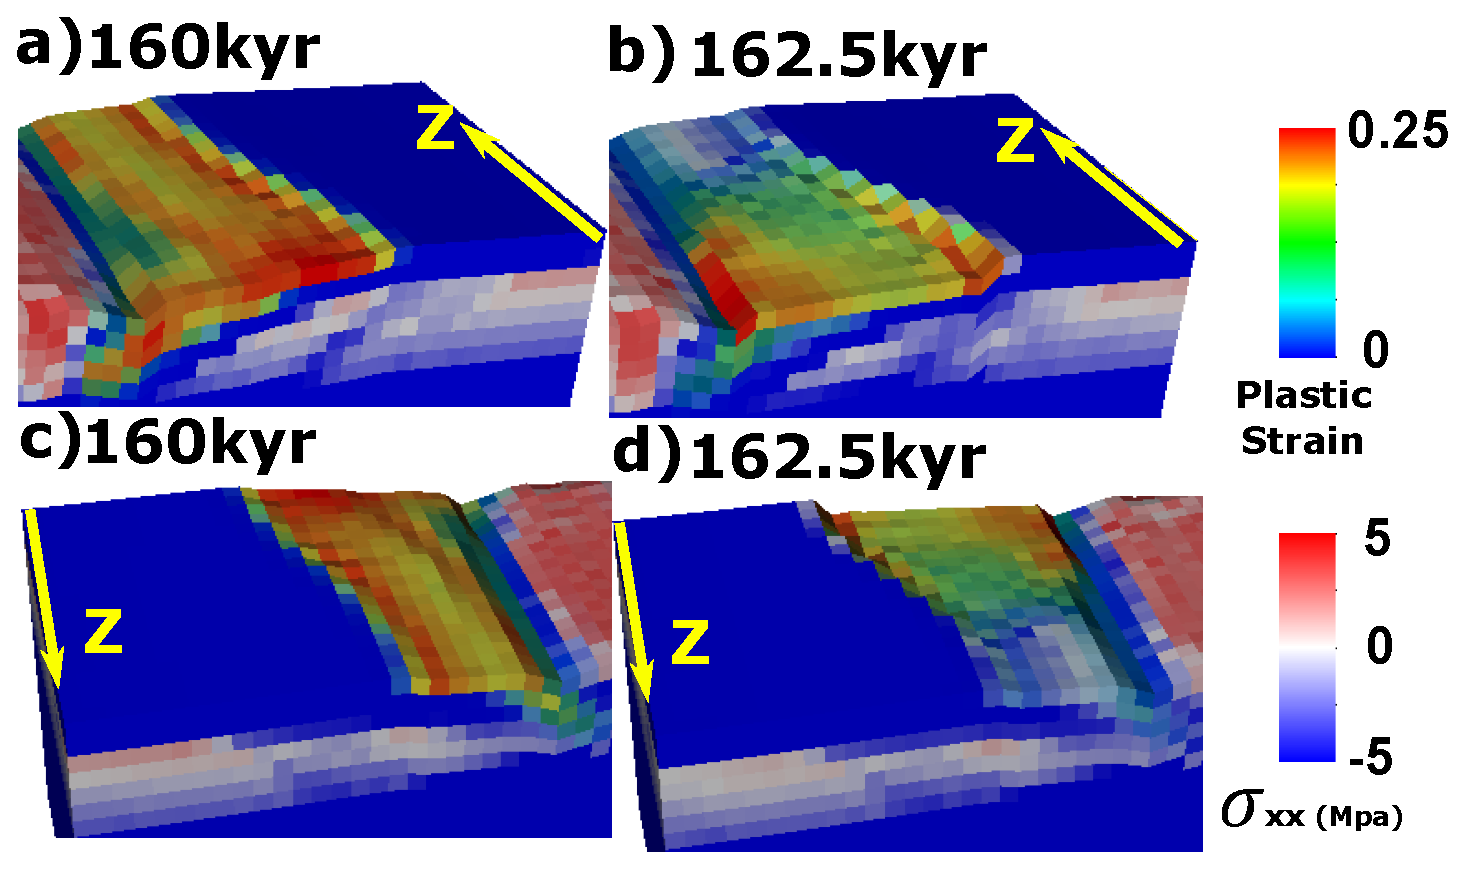
\includegraphics[width=0.6\textwidth]{./Figures/fig_Results4_6_sqrt_cut_back_bending_drop.eps}
  \caption{M28SqrtT1 (Table~\hyperref[Tab1_1]{\ref{Tab1_1}}). Bending stress drop (a versus b) at the lower M side due to the cut-back. No bending stress drop (c versus d) at the higher M side as a comparison.}
 \label{fig_Results4_6}
\end{figure}
\fi
%Mass wasting only happens at the lower M side as indicated by the red-colored (i.e., high-speed) block (``a large slump block'' \citep{Smith2014}) of Figure~\hyperref[fig_Results4_4]{\ref{fig_Results4_4}.b,e (velocity)}. The tensional stress due to bending is released at the lower M side (0.2 $<$ M $<$ 0.57) (Figure~\hyperref[fig_Results4_6]{\ref{fig_Results4_6}.a compared to b}), however, the cut-back does not propogates to the higher M side and the tensional bending stress is not released (Figure~\hyperref[fig_Results4_6]{\ref{fig_Results4_6}.c compared to d}). This difference in the bending stresses between the lower and higher M sides is partly due to the decouple between lower and higher M side hanging walls. In addition, once the cut back happens at 162.5 kyr, the $\sigma_{xy}$, $\sigma_{xz}$ and $\sigma_{xx}$ are released (Figure~\hyperref[fig_Results4_4]{\ref{fig_Results4_4}.e (fourth and fifth row: $\sigma_{xy}$ and $\sigma_{xz}$)}). %After the cut back, the termination of the detachment fault recedes backwards for about 7 km towards the ridge axis (Figure~\hyperref[fig_Results4_4]{\ref{fig_Results4_4}.f (third row: plastic strain)}).% (termination fronts are always consistent with tension stresses in $\sigma_{xx}$ and $\sigma_{zz}$ as well as with plastic strain front(due to healing, high plastic strain region corresponds only to region with continuously deformation) (Figure~\hyperref[fig_Results4_3_1]{\ref{fig_Results4_3_1}} and Figure~\hyperref[fig_Results4_3_2]{\ref{fig_Results4_3_2}})).
% because $\sigma_{xy}$ always accummulates immediately beneath the normal fault interface. The red $\sigma_{xz}$ on the positive $x$-axis direction of the new termination is due to the along ridge axis variatioin in the rate of fault slip.  

\iffalse
\begin{figure}[h]
  \centering
    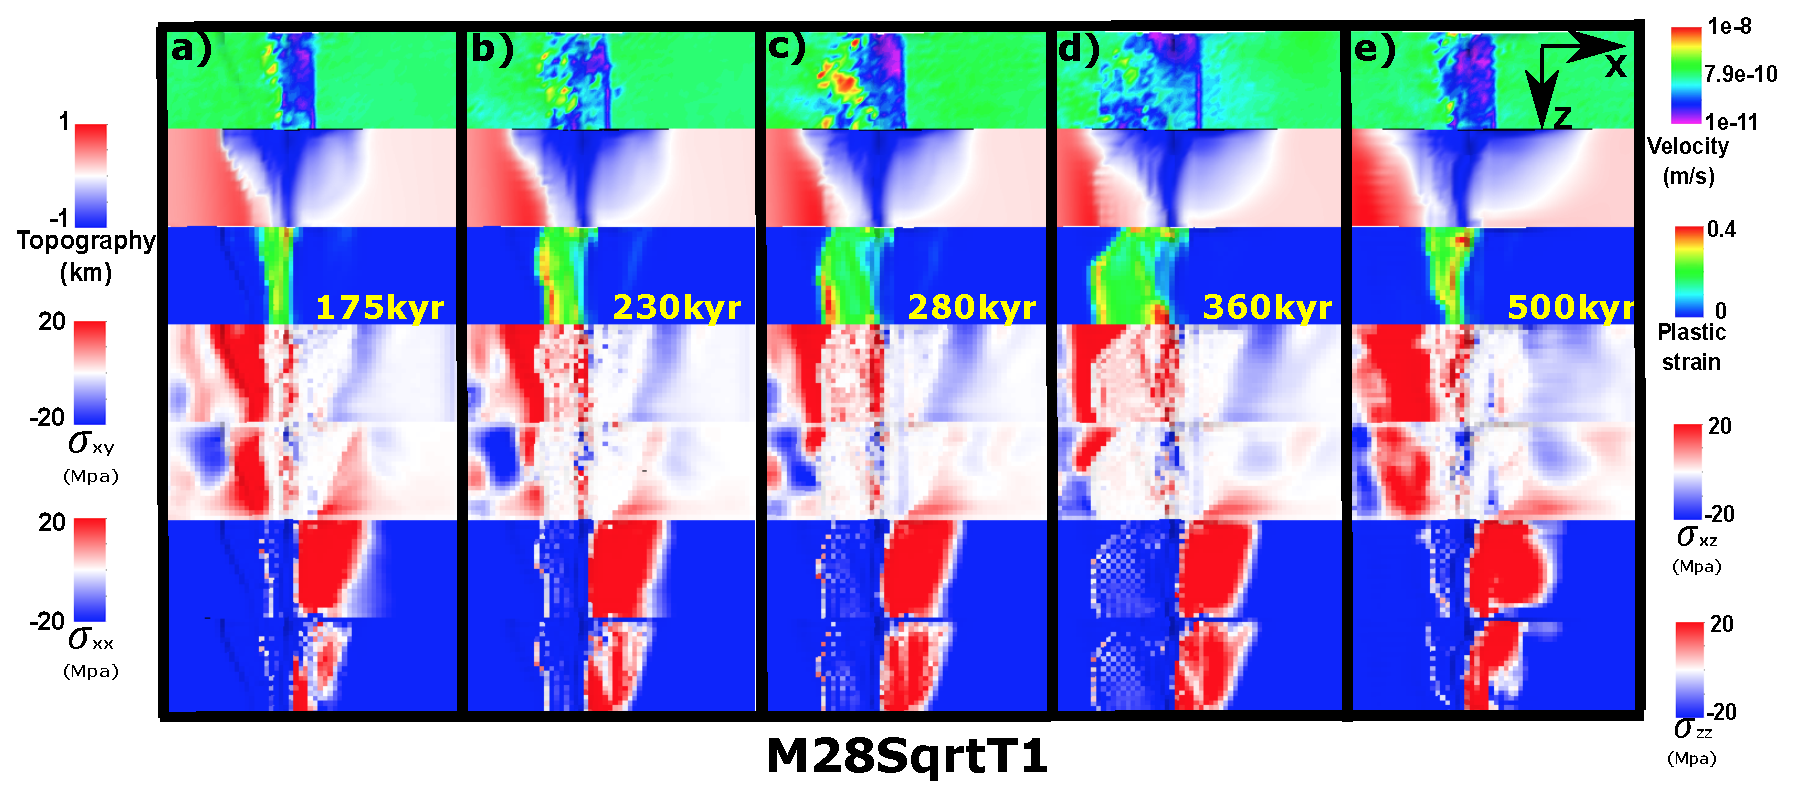
\includegraphics[width=1.0\textwidth]{./Figures/fig_Results4_9_sqrt_cut_back_new_fault_chase.eps}
  \caption{New fault front chase after cut-back.}
 \label{fig_Results4_9}
\end{figure}
\fi
\iffalse
Immediately after an event of mass wasting, the fault trace jumps towards the ridge axis (Figure~\hyperref[fig_Results4_4]{\ref{fig_Results4_4}.d versus f (third row: plastic strain)}). 
%This behavior helps maintain a high angle normal fault. 
Then, $\sigma_{xy}$ and $\sigma_{xz}$ soon \annote[EC]{fill in the area}{What do you mean by ``stresses filling an area''?} between cut-back created fault scarp and the new termination (Figure~\hyperref[fig_Results4_4]{\ref{fig_Results4_4}.f (fourth and fifth row: $\sigma_{xy}$ and $\sigma_{xz}$)}. \note[EC]{don't understand the rest of this paragraph.}
After that, the termination at the higher M side extends faster and further than the lower M side (Figure~\hyperref[fig_Results4_9]{\ref{fig_Results4_9}.a$\sim$d}). This is because during the cut-back, tensional stress due to bending is released at the lower M side but continues to accummulate at the higher M side. At the lower M side, it needs time to reach the previous tensional stress state and then starts from there to pull the new termination away from the ridge axis. While at the higher M side the increasing tensional stress directly leads to a fast extending termination.
\fi
%\add[XT]{One question is, how to explain that the fault front is moving much faster than the initial abandoned breakaway? New fault front soon reach the old breakaway.}

%This phenomenon is responsible for the corrugations observed. It creates an ``X'' shape ``scan'' that first ``scan'' the topography with the faster low M side (Figure~\hyperref[fig_Results4_4]{\ref{fig_Results4_4}.d and e}) and then ``scan'' with the faster higher M side (Figure~\hyperref[fig_Results4_9]{\ref{fig_Results4_9}.c and d}). This results in a evolving curved termination that produces mullion structures (Figure~\hyperref[fig_Results4_9]{\ref{fig_Results4_9}.d}). \note[EC]{Can't follow what you say.}  

\subsubsection{Hourglass-shaped median valley}

All the models with M variation develop an hourgalss-shaped median valley although the geometry of the median valley changes with time and with the functional forms and ranges of M variation. %As shown in Figure~\hyperref[fig_Results_3_2_hourglass_evolution]{\ref{fig_Results_3_2_hourglass_evolution}.a}, initially, 
A median valley of the M28Sqrt model initially has a uniform width along the ridge but is deeper on the lower M side where normal faults first form (Figure~\hyperref[fig_Results_3_2_hourglass_evolution]{\ref{fig_Results_3_2_hourglass_evolution}.a}). By $\sim$100 kyr, the fault on right hand side of the ridge axis does not propagate to the higher M side of the ridge and becomes inactive (Figure~\hyperref[fig_Results_3_2_hourglass_evolution]{\ref{fig_Results_3_2_hourglass_evolution}.b}). It produces a depressed topography curve following the inactive fault trace, which is further away from the ridge axis at the lower M side but closer to ridge axis at the higher M side. On the other side of the ridge axis, as the active fault rotates to a lower dip angle, breakaways at the lower M side move further away from the ridge axis than the breakaways at the higher M side. This along-ridge variation in the location of the breakaways act as another boundary of the hourglass on the left. %Both boundaries are extended following the spreading plates. 

\begin{figure}[h]
  \centering
    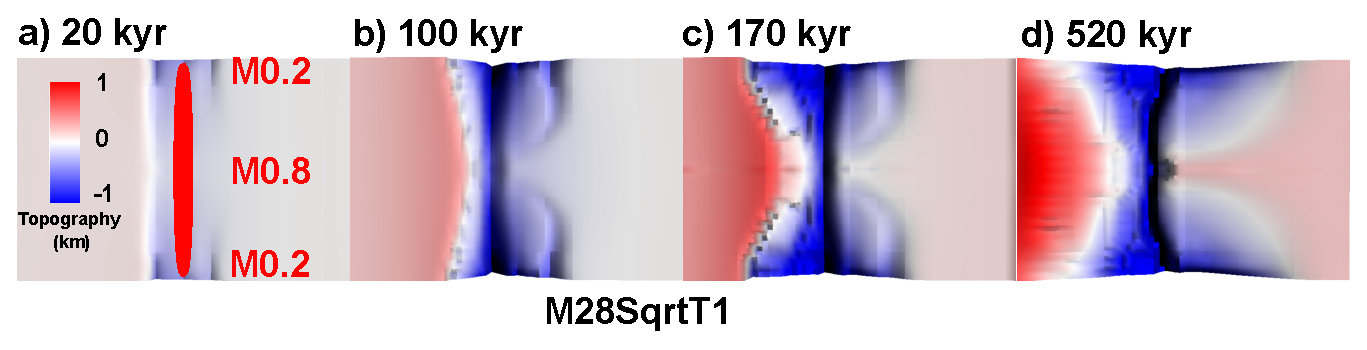
\includegraphics[width=1.0\textwidth]{./Figures/fig_Results_3_2_hourglass_evolution.eps}
  \caption[Bird's-eye view of the evolution of the hourglass-shaped median valley.]{Bird's-eye view of the evolution of the hourglass-shaped median valley. It is generated by attaching the topography of the M28SqrtT1 model to its mirror image by assumming symmetrical M variation (0.2 to 0.8 to 0.2). }
 \label{fig_Results_3_2_hourglass_evolution}
\end{figure}

By $\sim$170 kyr (Figure~\hyperref[fig_Results_3_2_hourglass_evolution]{\ref{fig_Results_3_2_hourglass_evolution}.c}), the hourglass-shaped median valley continues to widen and deepen. Since the area of the cross section along the ridge inside the hourglass-shaped median valley is approximately inversely proportional to the local M values, the shape of the hourglass varies with different ranges and functional forms of M variations.

In addition, the further depression inside the median valley is mostly due to the elastic deformation from crustal extension. As shown in Figure~\hyperref[fig_Results4_7]{\ref{fig_Results4_7}}, the $\sigma_{xx}$ in the median valley is higher because the brittle crust is thinner, when same amount of force propagates from far field extension to the median valley, the stress increases. This increased $\sigma_{xx}$ is responsible for the further depression and extension of the median valley on the side of the ridge axis with no active faulting (Figure~\hyperref[fig_Results_3_2_hourglass_evolution]{\ref{fig_Results_3_2_hourglass_evolution}.d}). For the median valley on the other side of the ridge axis, mass wasting between the breakaways and the ridge axis results in further lowering of topography (Figure~\hyperref[fig_Results4_4]{\ref{fig_Results4_4}.d versus e (topography)}). 

\begin{figure}[h]
  \centering
    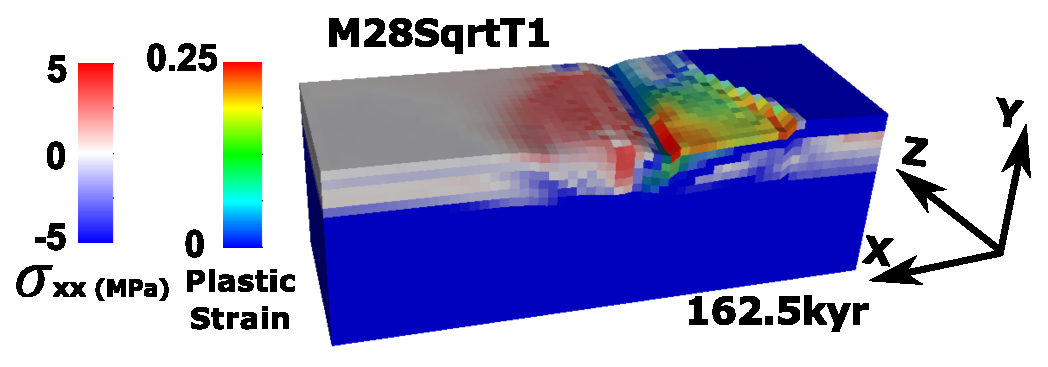
\includegraphics[width=0.6\textwidth]{./Figures/fig_Results4_7_sqrt_cut_back_conjugate_Sxx.eps}
  \caption{Higher $\sigma_{xx}$ shows inside the median valley on the positive $x$-axis direction of the ridge axis. }
 \label{fig_Results4_7}
\end{figure}

\subsubsection{Corrugations and mullion structures}

Both corrugations and mullion structures are linear structures parallel to the spreading direction. As shown in Figure~\hyperref[fig_Results1_1]{\ref{fig_Results1_1}.f}, at the M $<$ 0.5 area on top of the OCC surface, corrugations show a uniform wavelength of $\sim$2 km with hundreds of meters in amplitude. At the higher M side of the ridge (Figure~\hyperref[fig_Results1_1]{\ref{fig_Results1_1}.g}), a mullion structure with a wavelength of $\sim$7 km shows up on the surface of the OCC. In spite of morphological similarity, corrugations and mullion structures have different formation mechanisms. 

\paragraph{Corrugations}
~\\
The corrugation starts at the breakaway as a response to tensile stress in the $z$-axis direction. As shown in Figure~\hyperref[fig_Results_3_2_6_corrugations_evolution]{\ref{fig_Results_3_2_6_corrugations_evolution}}, when the plastic strain reaches or excedes 0.1 (red color), base on type 1 weakening, the cohesion decreases to 4 MPa. With a 30 $\degree$ friction angle, tensile failure is declared when the $\sigma_{zz}$ reaches $\sim$7 MPa (yellow color).

\begin{figure}[h]
  \centering
    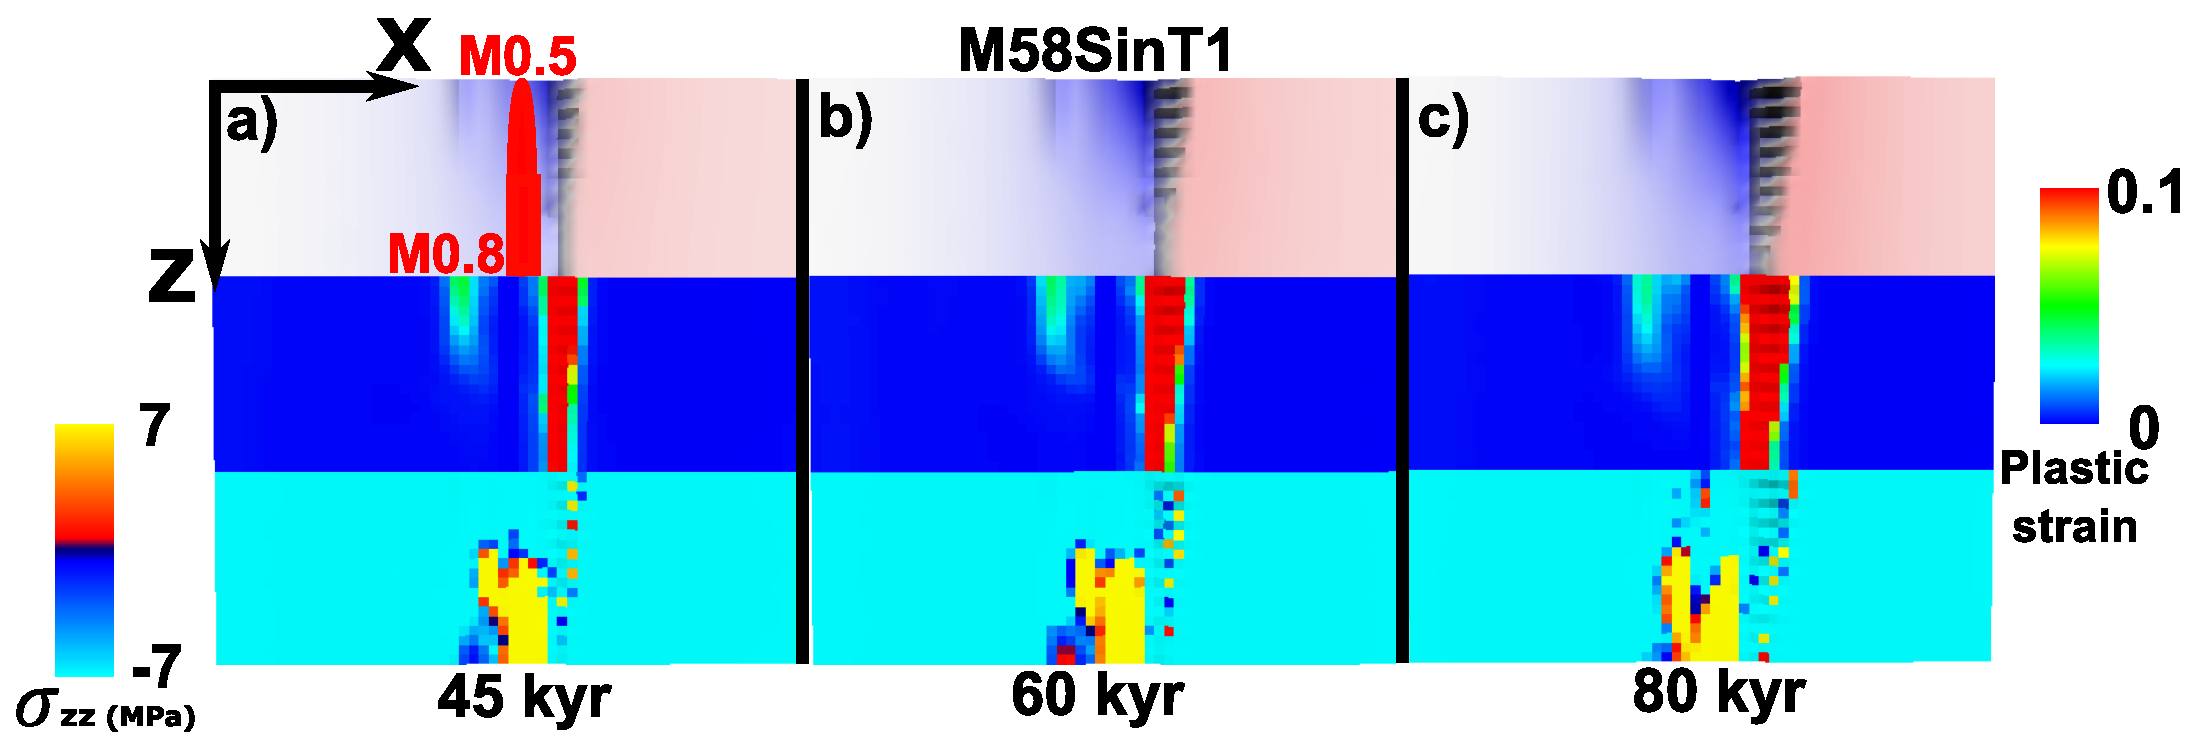
\includegraphics[width=1.0\textwidth]{./Figures/fig_Results_3_2_6_corrugations_evolution.eps}
  \caption[Bird's-eye view of the evolution of the corrugations.]{Bird's-eye view of the evolution of the corrugations. Color scales for the topography is the same as Figure~\hyperref[fig_Results1_1]{\ref{fig_Results1_1}}.}
 \label{fig_Results_3_2_6_corrugations_evolution}
\end{figure}

The tensile stress is generated by the asynchronous faulting along the ridge. Faulting initiates earlier at the lower M side of the ridge. As the fault offsets more on the lower M side than on the higher M side, the footwall of the fault rotates and get uplifted more on the lower M side. This relative displacement between the footwalls along the ridge generates the isochron-parallel tensional stress $\sigma_{zz}$. Since $\sigma_{zz}$ follows along the moving tip of the plastic strain, the plastic srain together with $\sigma_{zz}$ generate tensile failure that propagates away from the ridge axis and thus produces the linear corrugations that are parallel to the spreading velocity. Detailed analysis along with simpler model experiments are given in the ``Discussion'' section.   

\iffalse
\note[EC]{These sentences would better fit in model comparison section or Discussion.}
Corrugations are observed in most of the models except for the constant M model M88ContT2 (Figure~\hyperref[fig_Results1_3]{\ref{fig_Results1_3}}). Among the models that have corrugations, the timing, location and the regularity of the corrugations varies. For example, corrugations in M58SinT1 shows up $\sim$45 kyr at the lower M side (0.5 $<$ M $<$ 0.65) (Figure~\hyperref[fig_Results_3_2_6_corrugations_evolution]{\ref{fig_Results_3_2_6_corrugations_evolution}.a)}). However, corrugations in M28LinT1 shows up much later at $\sim$240 kyr at the lower M side (0.2 $<$ M $<$ 0.38) (Figure~\hyperref[fig_Results1_1]{\ref{fig_Results1_1}.c}). For M28LinT1, the corrugations are mostly formed at the lower M side (M $<$ 0.5) through time and they are less regular along the ridge ((Figure~\hyperref[fig_Results1_1]{\ref{fig_Results1_1}.h})). But the corrugations in M58SinT1 appear along the whole ridge and shows regularly alternative undulations with a wavelength of $\sim$1 km (Figure~\hyperref[fig_Results_3_2_6_corrugations_evolution]{\ref{fig_Results_3_2_6_corrugations_evolution}.c)}). 
\fi

\paragraph{Mullion structures}
~\\
Mullion structures observed in the models are formed by the along-ridge variation in the location of the termination due to the evolution of faulting. They usually appear where the termination is closer to the ridge axis. The shape of the footwall follows the trace of the termination as it is exhumed to the surface. Where the termination is bent inward to the ridge axis, an ``initial dome'' (Figure~\hyperref[fig_Results_3_2_6_mullion_evolution]{\ref{fig_Results_3_2_6_mullion_evolution}.a}) is produced once the footwall is exhumed to the seafloor. The wavelength of the mullion structure is determined by the shape of the termination. If the pattern of the termination lasts for a long time and the footwall of the detachment fault keeps being exhumed to the surface following the trace of the detachment fault termination, a mullion structure is produced (Figure~\hyperref[fig_Results_3_2_6_mullion_evolution]{\ref{fig_Results_3_2_6_mullion_evolution}.b}). 

\begin{figure}[h]
  \centering
    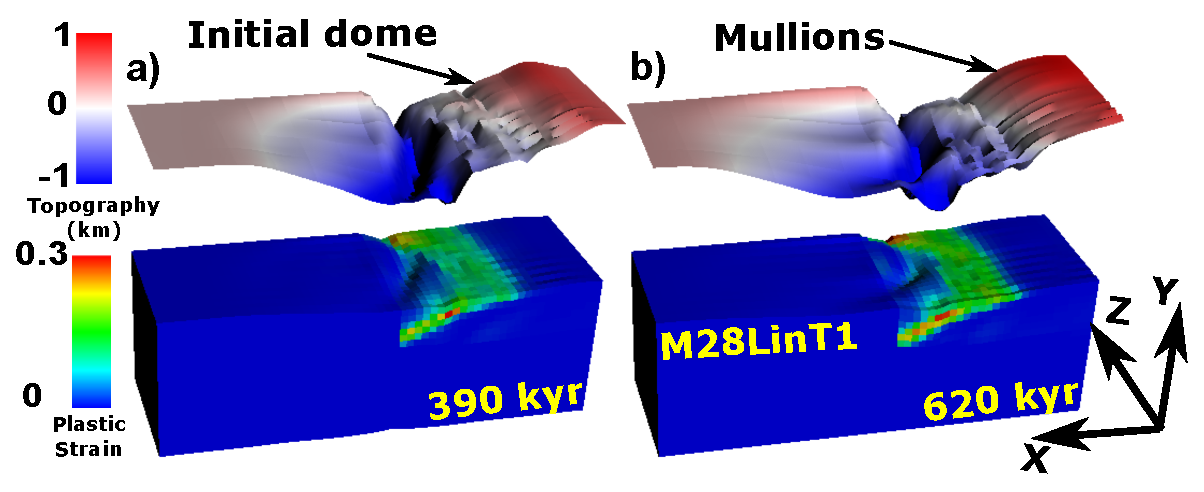
\includegraphics[width=1.0\textwidth]{./Figures/fig_Results_3_2_6_mullion_evolution.eps}
  \caption{Evolution of mullion structures.}
 \label{fig_Results_3_2_6_mullion_evolution}
\end{figure}

\subsection{Effects of the functional forms of M variation}

\subsubsection{M28T1}

Major differences among M28LinT1, M28SinT1 and M28SqrtT1 lie in the model behaviors in terms of the inward fault jump, the mass wasting and the hourglass-shaped median valley. None of the three models show fault alternation. Figure~\hyperref[fig_Results3_1]{\ref{fig_Results3_1}} shows M variations of three kinds of functional forms.

\begin{figure}[h]
  \centering
    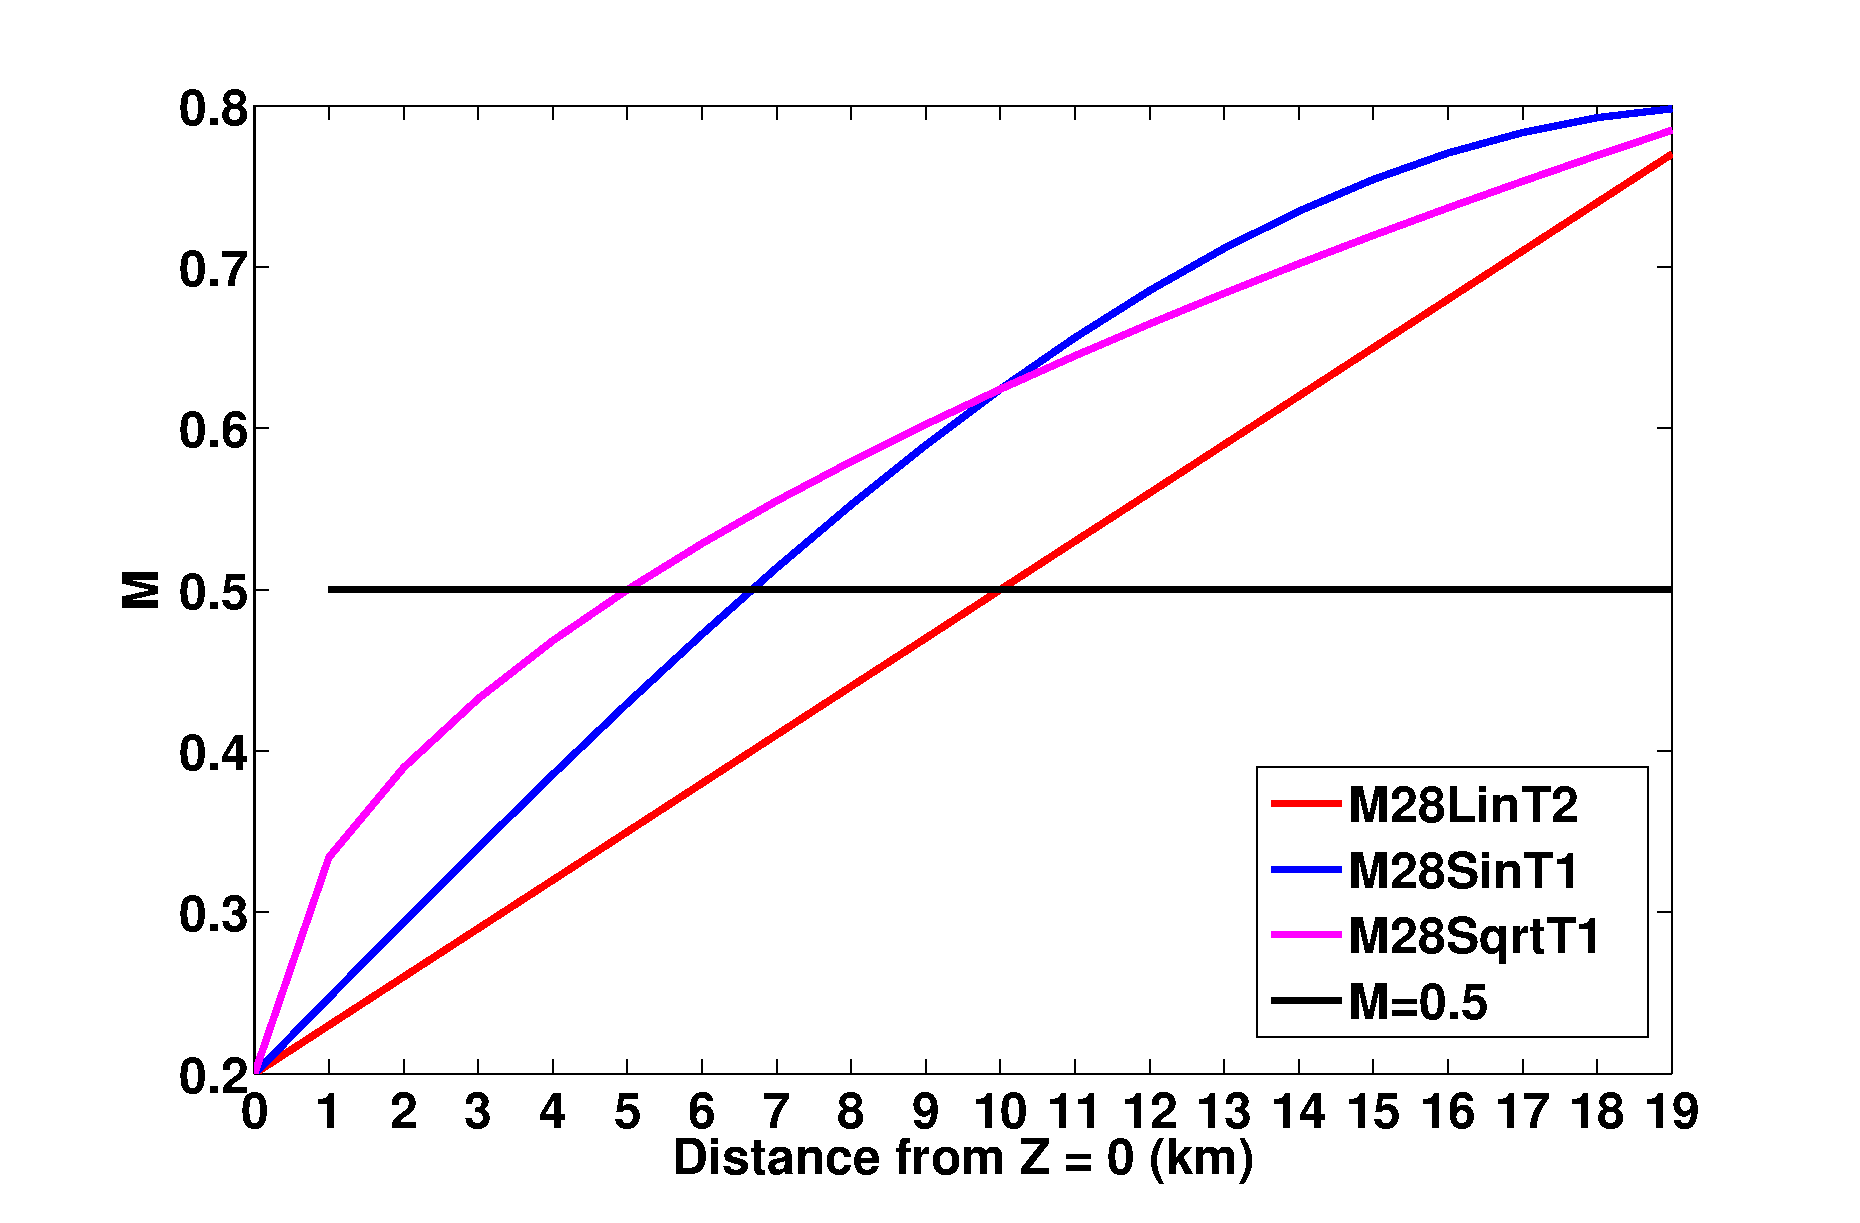
\includegraphics[width=0.8\textwidth]{./Figures/fig_Results_3_3_M_variation.eps}
  \caption[Three functional forms of M variation.]{Three functional forms of M variation. M begins to exceed the M $=$ 0.5 black line at Z=10 km, 7 km, 5 km for M28LinT1, M28SinT1 and M28SqrtT1 respectively.}
 \label{fig_Results3_1}
\end{figure}   

\paragraph{Inward fault jump}\label{para_InwardFaultJump}
~\\
Only the linear (M28LinT1) and sinusoidal (M28SinT1) models have inward fault jump. Sqaure root model (M28Sqrt) does not have inward fault jump because during mass wasting, termination of the detachment fault retreats backward toward the ridge axis and the detachment fault is maintained near the ridge axis.

Comparing linear and sinusoidal models, timing and dimension of the inward jumping faults are different. For the linear functional form, the inward fault jump at the higher M side starts accommodating most of the extension at $\sim$900 kyr and replaces the initial detachment fault (Figure~\hyperref[fig_Results4_2]{\ref{fig_Results4_2}}, Figure~\hyperref[fig_Results1_1]{\ref{fig_Results1_1}.f}). It nucleates from the ridge center where M $=$ 0.5 and then propagates to the M $=$ 0.8 end with a length of $\sim$11 km. 
 %This secondary fault creates another dome with initial composition likely to be volcanic rather than ultramafic, however, as it evolves, if it can last long enough to cut through the whole crust, mantle materials might exhume to the surface. The composition of the domes observed at Kane magamullions is similar to this mechanism between ultramafic babel dome and eastern to it the crustal inside-corner high.  its spatial distribution is at M$>0.5$ region.
For the sinusoidal functional form, the inward fault jump takes the place of the initial detachment fault earlier at $\sim$550 kyr with a length of 14 km (Figure~\hyperref[fig_Results4_2]{\ref{fig_Results4_2}}).

\begin{figure}[h]
  \centering
    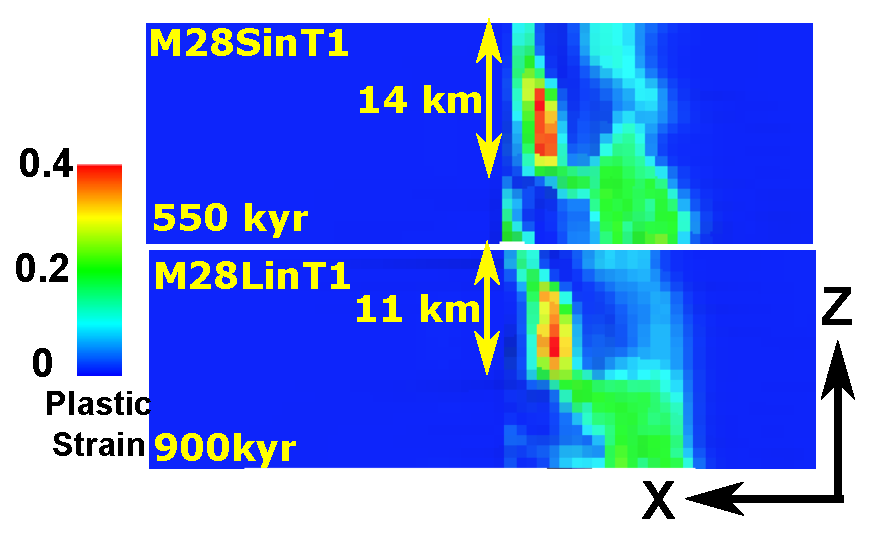
\includegraphics[width=0.6\textwidth]{./Figures/fig_Results4_2_secondary_fault_length_comparison1.eps}
  \caption{Bird's-eye view for comparing the length and timing of inward fault jump.}
 \label{fig_Results4_2}
\end{figure}   

The timing difference between the linear and sinusoidal models is because M28SinT1 consistently has a higher M value than the M28LinT1 (Figure~\hyperref[fig_Results3_1]{\ref{fig_Results3_1}}), which results in the initial detachment fault at the higher M side (M $>$ 0.5) of M28SinT1 being pushed off axis faster than M28LinT1 and thus forming an earlier inward fault jump. The length difference is because M28SinT1 has a greater length along the ridge axis of M $\ge$ 0.5 (Figure~\hyperref[fig_Results3_1]{\ref{fig_Results3_1}}). 
%\vspace{2cm}
\paragraph{Mass wasting}
~\\
Mass wasting only happens in the M28SqrtT1 model. Qualitatively, it is because M28Sqrt has a much higher value of $\frac{\partial M}{\partial Z}$ at the lower M side (Figure~\hyperref[fig_Results_3_3_1_M_type_plot_dM_dZ]{\ref{fig_Results_3_3_1_M_type_plot_dM_dZ}}), which implies a larger along ridge shear stress $\sigma_{xz}$ as well as a larger difference in $\sigma_{xy}$ along the ridge that result in the decoupling between the higher and lower M sides hanging walls. 

\begin{figure}[h]
  \centering
    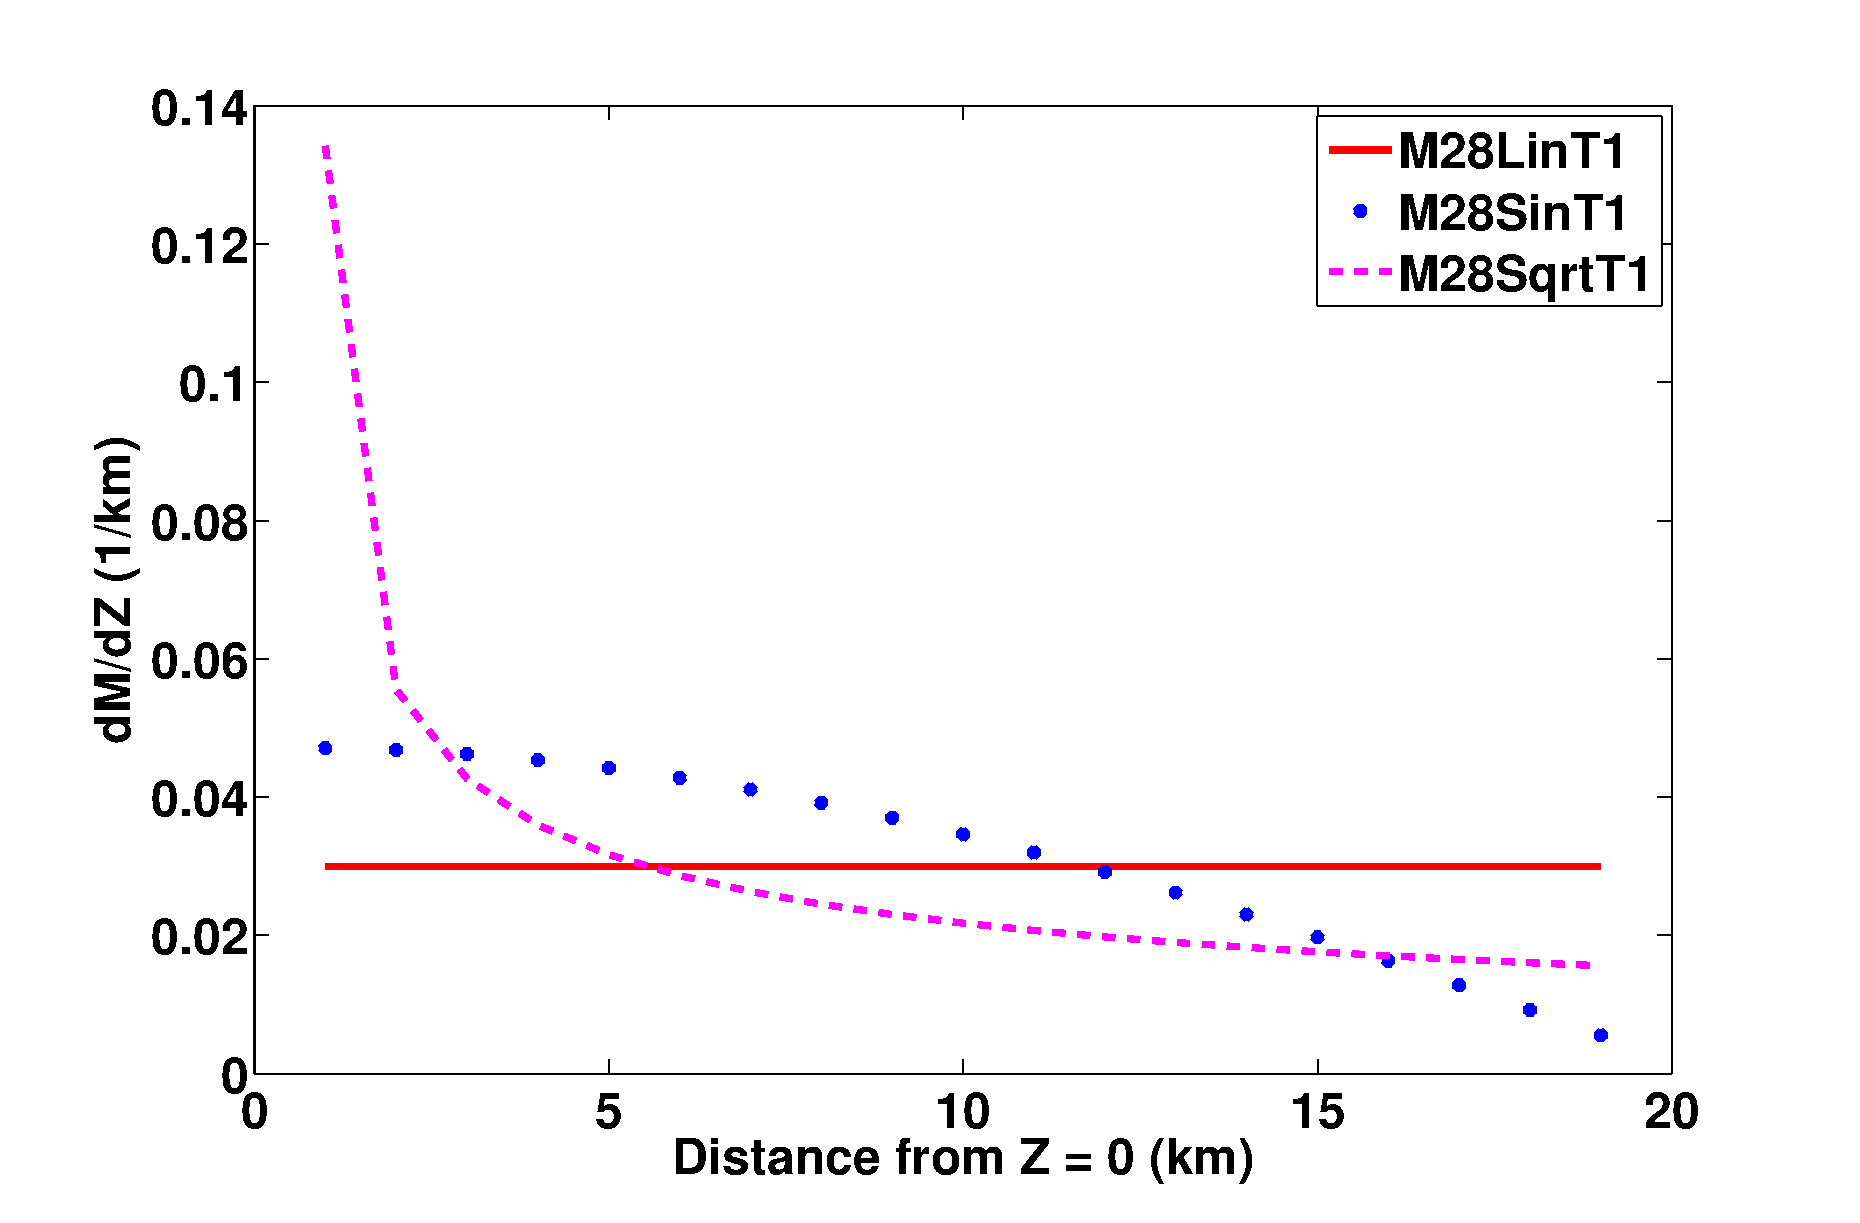
\includegraphics[width=0.8\textwidth]{./Figures/fig_Results_3_3_1_M_type_plot_dM_dZ.eps}
  \caption{$\partial M/ \partial Z$ comparision.}
 \label{fig_Results_3_3_1_M_type_plot_dM_dZ}
\end{figure}  

\iffalse
\begin{figure}[h]
  \centering
    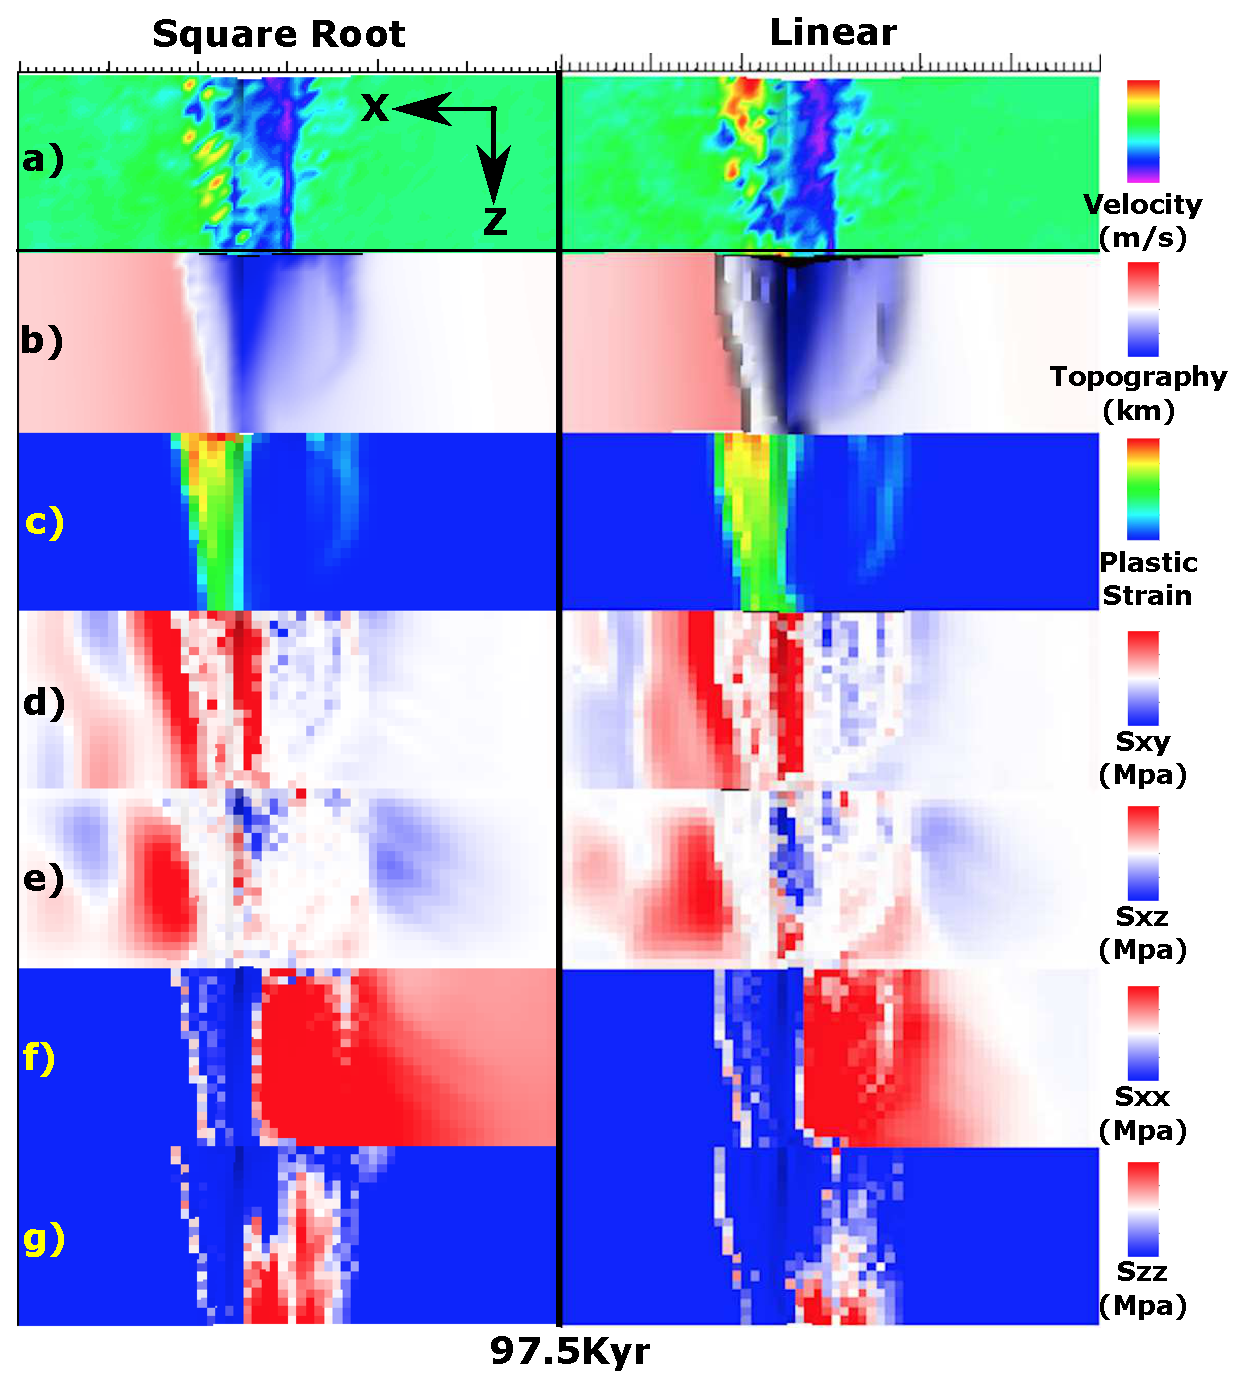
\includegraphics[width=0.6\textwidth]{./Figures/fig_Results4_3_sqrt_vs_lin_cut_back_97kyr.eps}
  \caption{M28LinT1 versus M28SqrtT1 (Table~\hyperref[Tab1_1]{\ref{Tab1_1}}) at 97 kyr. View from top of the model.}
 \label{fig_Results4_3_1}
\end{figure}  

\begin{figure}[h]
  \centering
    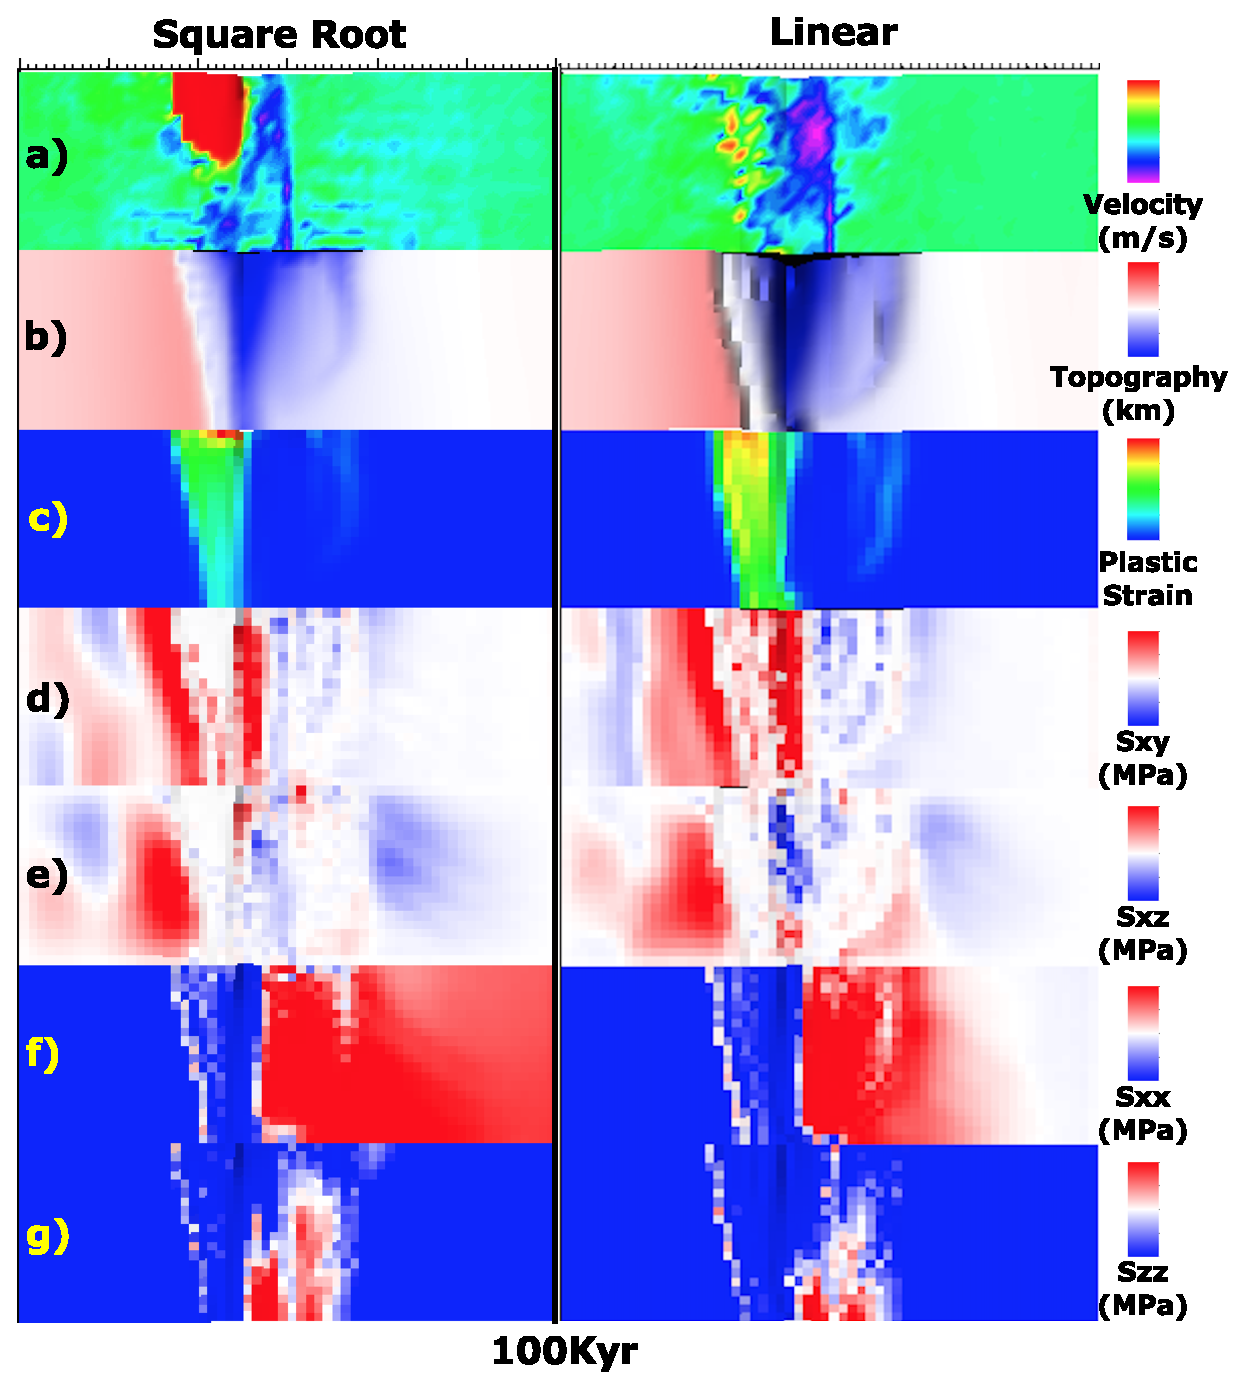
\includegraphics[width=0.6\textwidth]{./Figures/fig_Results4_3_sqrt_vs_lin_cut_back_100kyr.eps}
  \caption{M28LinT1 versus M28SqrtT1 (Table~\hyperref[Tab1_1]{\ref{Tab1_1}}) at 100 kyr. View from top of the model.}
 \label{fig_Results4_3_2}
\end{figure} 
\fi

\paragraph{Hourglass-shaped median valley}
~\\
As shown in Figure~\hyperref[fig_Results_3_3_1_hourglass]{\ref{fig_Results_3_3_1_hourglass}}, differences among the three models are identified. At 160 kyr, median valley for M28SinT1 has the smallest cross sectional ($x$-$y$) area at the higher M side (center of the ridge segment). Whereas at the lower M side,  M28SqrtT1 has the smallest cross section. This is because the cross-section inside the median valley is inversely proportional to the local M value along the ridge. Moreover, the breakaways at the lower M sides for M28LinT1 and M28SinT1 bend to parallel to the ridge axis while the breakaway for M28SqrtT1 moves further away from the ridge axis. In addition, M28SinT1 has a trough inside the median valley with the highest curvature. At 500 kyr, M28SinT1 has the narrowest median valley at the higher M side and the high topography zone on the left-hand side of the ridge axis is the widest. Integrating the topography below initial elevation (0 km) inside the median valleys of the three models, M28Sin has the lowest value of integration because it has the largest amount of magma supply of M $>$ 0.5 (Figure~\hyperref[fig_Results3_1]{\ref{fig_Results3_1}}). In addition, the termination of the detachment fault of M28SqrtT1 has the highest curvature at the lower M sides. All these model behaviors correspond to the M variation (Figure~\hyperref[fig_Results3_1]{\ref{fig_Results3_1}}).

\begin{figure}[h]
  \centering
    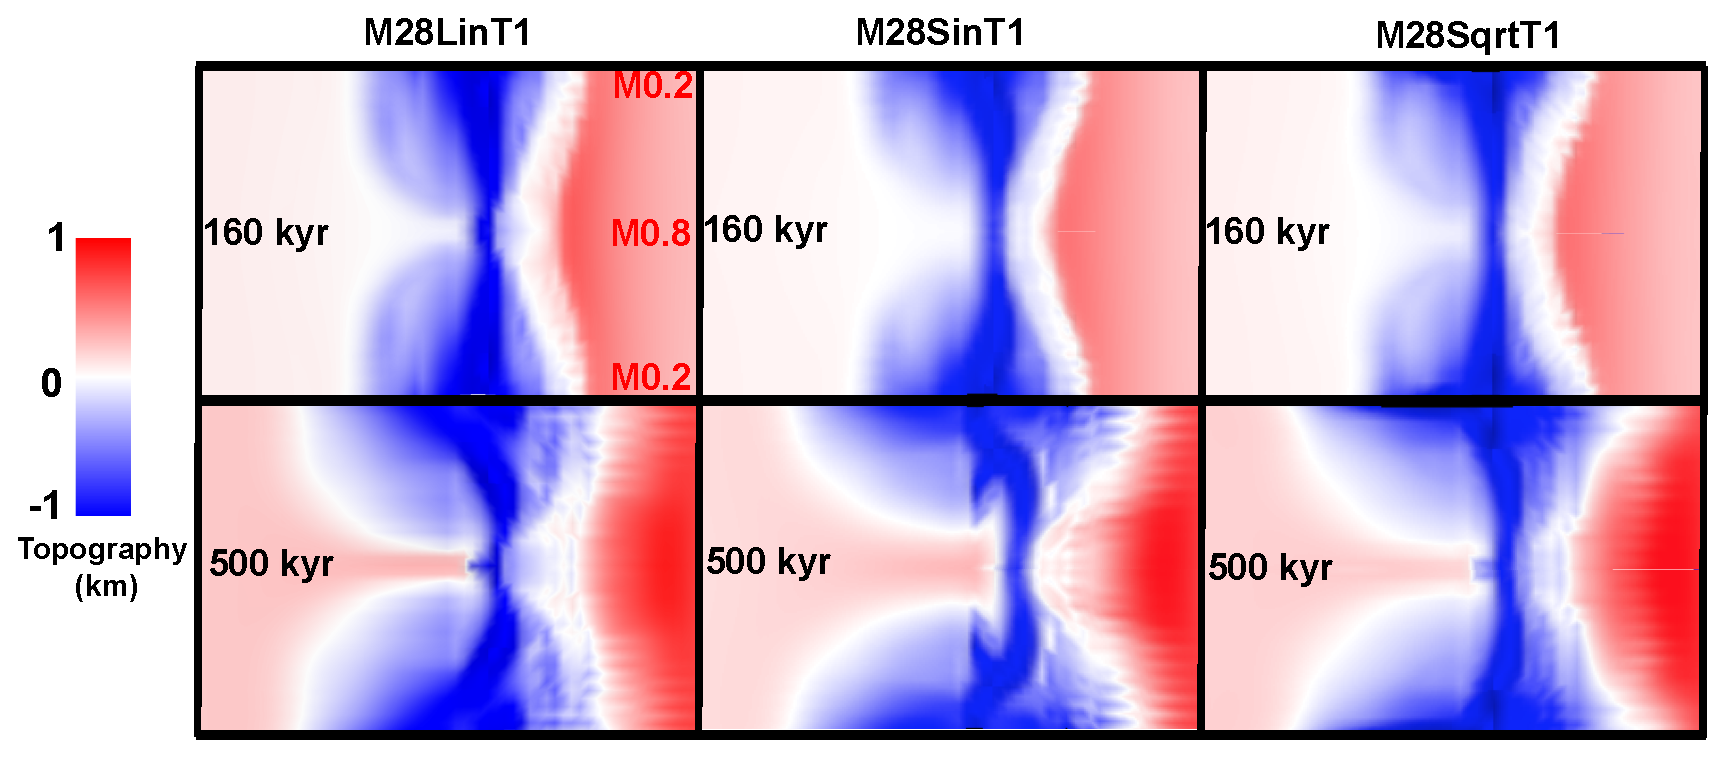
\includegraphics[width=1.0\textwidth]{./Figures/fig_Results_3_3_1_hourglass.eps}
  \caption[Bird's-eye view of the topograpy.]{Bird's-eye view of the topograpy. (Original and mirror images are put together assumming symmetrical M variation.) }
 \label{fig_Results_3_3_1_hourglass}
\end{figure} 

\subsubsection{M58T2}

Among M58LinT2, M58SinT2 and M58SqrtT2, the major difference lies in ``fault alternation''. Except for the constant M model M88ContT2, among all the models, only the models with type 2 weakening and M ranges from 0.5 to 0.8 (M58) have fault alternation. However, M58LinT2 does not produces alternating fault during the 1.1 Myr model time. Instead, one detachment fault lasts until $\sim$300 kyr when the inward fault jump happens at the higher M side (0.65 $<$ M $<$ 0.8) and replaces the initial detachment fault. This provides a lower limit of $\bar{M}$ that prevents fault alternation and alows a long-lived detachment fault to produce an OCC. As shown in Table~\hyperref[Tab_3_3_average_M]{\ref{Tab_3_3_average_M}}, the lower limit is 0.6425 for M58LinT2. Detail analysis of the fault alternation is given in ``Discussion''.

\begin{table}[h!]
\begin{small}
\begin{center}
\begin{tabular}{|l|p{1.2cm}|p{1.2cm}|p{1.2cm}|}
\hline
\diagbox[width=8em]{Function}{M range}&
M28&M57&M58\\
\hline
Linear & \cellcolor{magenta!60}0.4850 & \cellcolor{magenta!60}0.5950 & \cellcolor{magenta!80}0.6425 \\
\hline
Sinusoidal & \cellcolor{magenta!60}0.5668 & \cellcolor{magenta!60}0.6223 & \cellcolor{green!60}0.6834   \\
\hline
Square root & \cellcolor{magenta!60}0.5837 & \cellcolor{magenta!60}0.6279 & \cellcolor{green!60}0.6918  \\
\hline
\end{tabular}
\end{center}
\end{small}
\caption{Average M values ($\bar{M}$) of the models. (The value is calculated by integrating M along the ridge axis and divided by the length (20 km) of the model domain in $z$-axis.)}
\label{Tab_3_3_average_M}
\end{table}

\subsection{Effects of the weakening rate}

\subsubsection{M57SinT1 versus M57SinT2}
~\\
Initially, both models develop normal faults on both sides of the ridge axis at the lower M side. In the model with the faster weakening rate (M57SinT1), faults propagate toward the higher M side and cut through the whole crust by 25 kyr but this process completes 25 kyr later in the model with slower weakening rate (M57SinT2). By $\sim$310 kyr, the inward fault jump appears at the higher M side (M $>$ 0.5908) of M57SinT2 whereas at M $<=$ 0.5908, the initial fault remains active (Figure~\hyperref[fig_Results_Weakenging_2]{\ref{fig_Results_Weakenging_2}.c and d}). However, when the weakening is fast (M57SinT1), mass wasting happens at $\sim$260 kyr and helps to maintain a relatively higher angle fault with a termination closer to the ridge axis. The initial fault remains and no inward fault jump forms (Figure~\hyperref[fig_Results_Weakenging_2]{\ref{fig_Results_Weakenging_2}.a and b}). In addition, the width of median valley at the lower M side is wider for M57SinT2 than M57SinT1 (Figure~\hyperref[fig_Results_Weakenging_2]{\ref{fig_Results_Weakenging_2}.c, d versus a, b}) because slower weakening (type 2) alows a more distributed tensional stress $\sigma_{xx}$ rather than fast weakening that once a fault establishes, larger amount of the tensional stress $\sigma_{xx}$ is released at the fault. The amplitude of the corrugations of M57SinT1 is larger than that of slower weakening M57SinT2. This is because faster weakening rate allows a faster decrease in the cohesion. As the cohesion reaches its minimum of 4 MPa ealier when the plastic strain accummulates to 0.1, tensile failure is easy to happen in the isochron parallel direction and produces the corrugations.  

\begin{figure}[h]
 \centering
  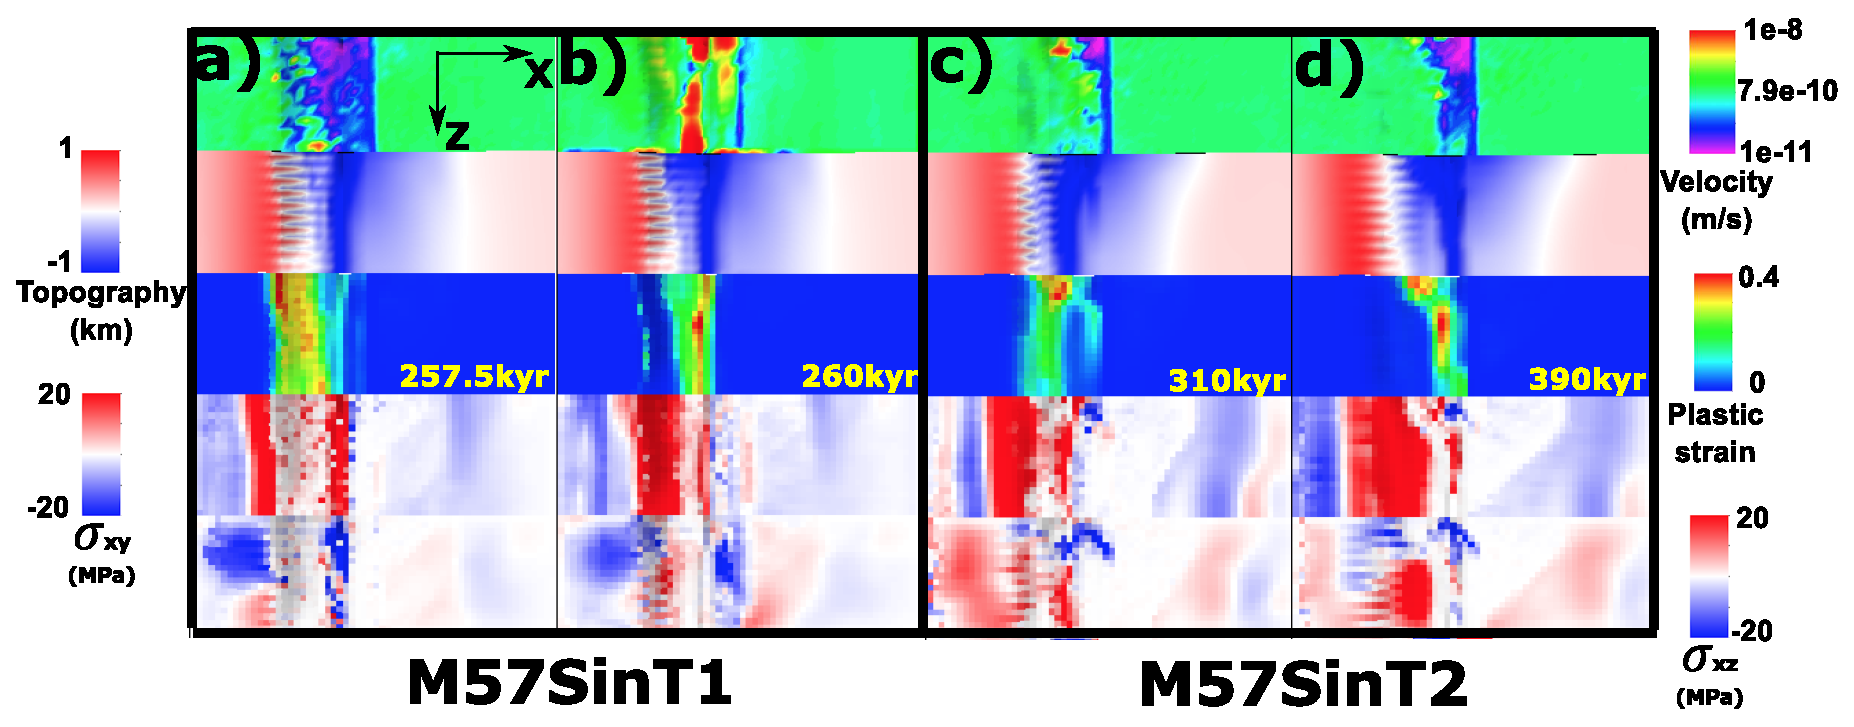
\includegraphics[width=1.0\textwidth]{./Figures/fig_Results_Weakening_2_M57SinT1VST2_CutbackVSsecondaryFault.eps}
 \caption{Bird's-eye view of M57SinT2 versus M57SinT1 (Table~\hyperref[Tab1_1]{\ref{Tab1_1}}).}
\label{fig_Results_Weakenging_2}
\end{figure}

\paragraph{M57SinT1}\label{para_M57SinT1}
~\\
For M57SinT1, by 400 kyr (Figure~\hyperref[fig_Results_Weakenging_3]{\ref{fig_Results_Weakenging_3}.a}), two antithetic faults form at the lower M side (0.5 $<$ M $<$ 0.6521) accommodating part of the plate extension. This makes the termination at the lower M side retreat backward to the ridge axis. By 530 kyr, the termination at the center of the ridge segment (M $=$ 0.6299$\sim$0.6618) moves further away from the ridge axis (Figure~\hyperref[fig_Results_Weakenging_3]{\ref{fig_Results_Weakenging_3}.b}). This curved termination leads to a curved topography aligning with it (white curve in the second row). By 740 kyr, another antithetic fault forms at the lower M side (Figure~\hyperref[fig_Results_Weakenging_3]{\ref{fig_Results_Weakenging_3}.c}). It doesn't take the place of initial fault and disappear soon, however, it again releases tensional stress and helps maintain a closer to ridge axis termination at the lower M side. By 1000 kyr (Figure~\hyperref[fig_Results_Weakenging_3]{\ref{fig_Results_Weakenging_3}.d}), an Atlantiss Massif shape OCC is produced (lower M side has a larger dome and higher M side has a smaller dome due to the along ridge termination evolution. Corrugations with wavelength varying from hundreds meters to kilometers are also produced.       

\begin{figure}[h]
 \centering
  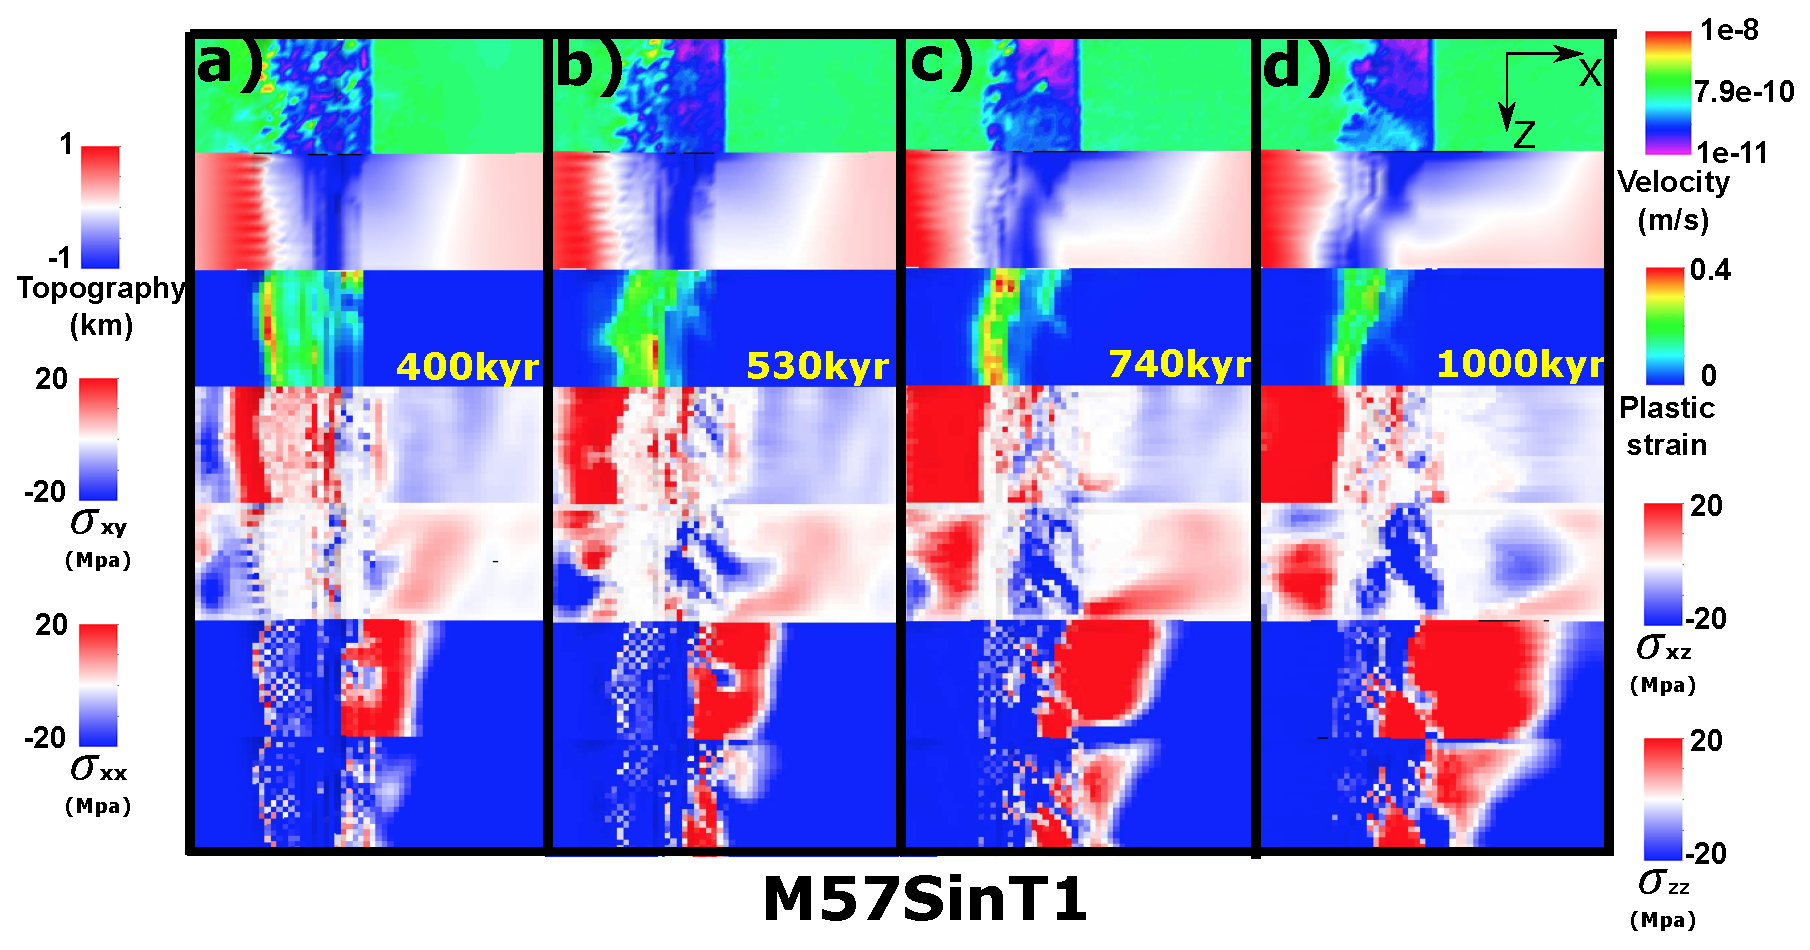
\includegraphics[width=1.0\textwidth]{./Figures/fig_Results_Weakening_3_M57SinT1_time_evolution.eps}
 \caption{Bird's-eye view of faulting and stresses evolution of M57SinT1.}
\label{fig_Results_Weakenging_3}
\end{figure}

\paragraph{M57SinT2}\label{para_M57SinT2}
~\\
For M57SinT2, instead of maintaining a detachment fault like M57SinT1, it produces inward fault jump at the higher M side. By 325 kyr (Figure~\hyperref[fig_Results_Weakenging_4]{\ref{fig_Results_Weakenging_4}.a}), an inward fault jump happens and takes the place of the initial detachment fault at the higher M side. Between 447.5 kyr (Figure~\hyperref[fig_Results_Weakenging_4]{\ref{fig_Results_Weakenging_4}.b}) and 450 kyr (Figure~\hyperref[fig_Results_Weakenging_4]{\ref{fig_Results_Weakenging_4}.c}), a small scale mass wasting happens and the termination recedes backward to the ridge axis. By 600 kyr, the termination at the higher M side extends further (Figure~\hyperref[fig_Results_Weakenging_4]{\ref{fig_Results_Weakenging_4}.d}). By 885 kyr, an inward fault jump happens at the higher M side (0.62 $<$ M $<$ 0.7) (Figure~\hyperref[fig_Results_Weakenging_4]{\ref{fig_Results_Weakenging_4}.e}). The width of the median valley at the lower M side keeps increasing due to the distributed $\sigma_{xx}$ (Figure~\hyperref[fig_Results_Weakenging_4]{\ref{fig_Results_Weakenging_4}.a$\sim$d}).

\begin{figure}[h]
 \centering
  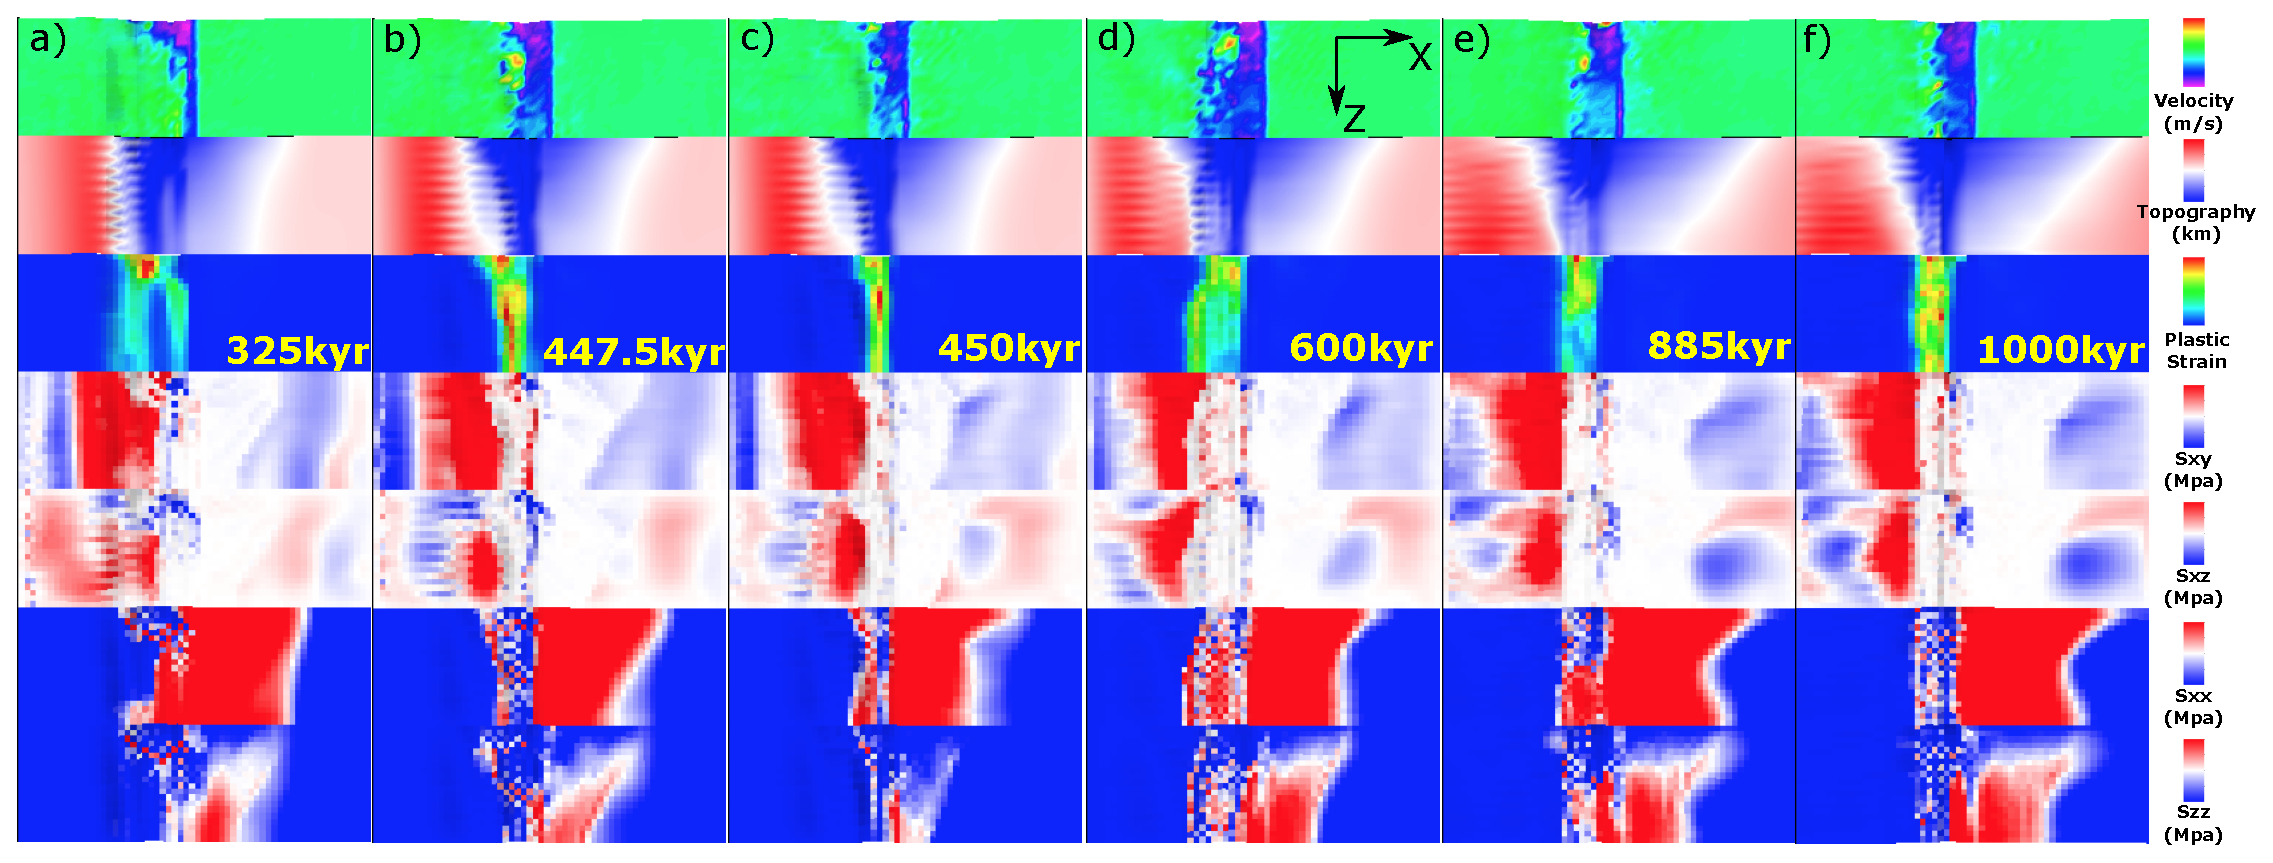
\includegraphics[width=1.0\textwidth]{./Figures/fig_Results_Weakening_4_M57SinT2_time_evolution.eps}
 \caption{Bird's-eye view of faulting and stresses evolution of M57SinT2.}
\label{fig_Results_Weakenging_4}
\end{figure}

\subsubsection{M58SinT1 versus M58SinT2}

A major difference between M58SinT1 and M58SinT2 is that only M58SinT2 has fault alternation.

\paragraph{M58SinT1}\label{para_M58SinT1}
~\\
During the 1 Myr extension of the model M58SinT1, 10 phases of the evolution of faulting are identified (Figure~\hyperref[fig_Results_Weakenging_5]{\ref{fig_Results_Weakenging_5}.a$\sim$j}). Antithetic faults, inward fault jumps, mass wasting happens with a rider block, corrugations and mullion structures produced.

\begin{figure}[h]
 \centering
  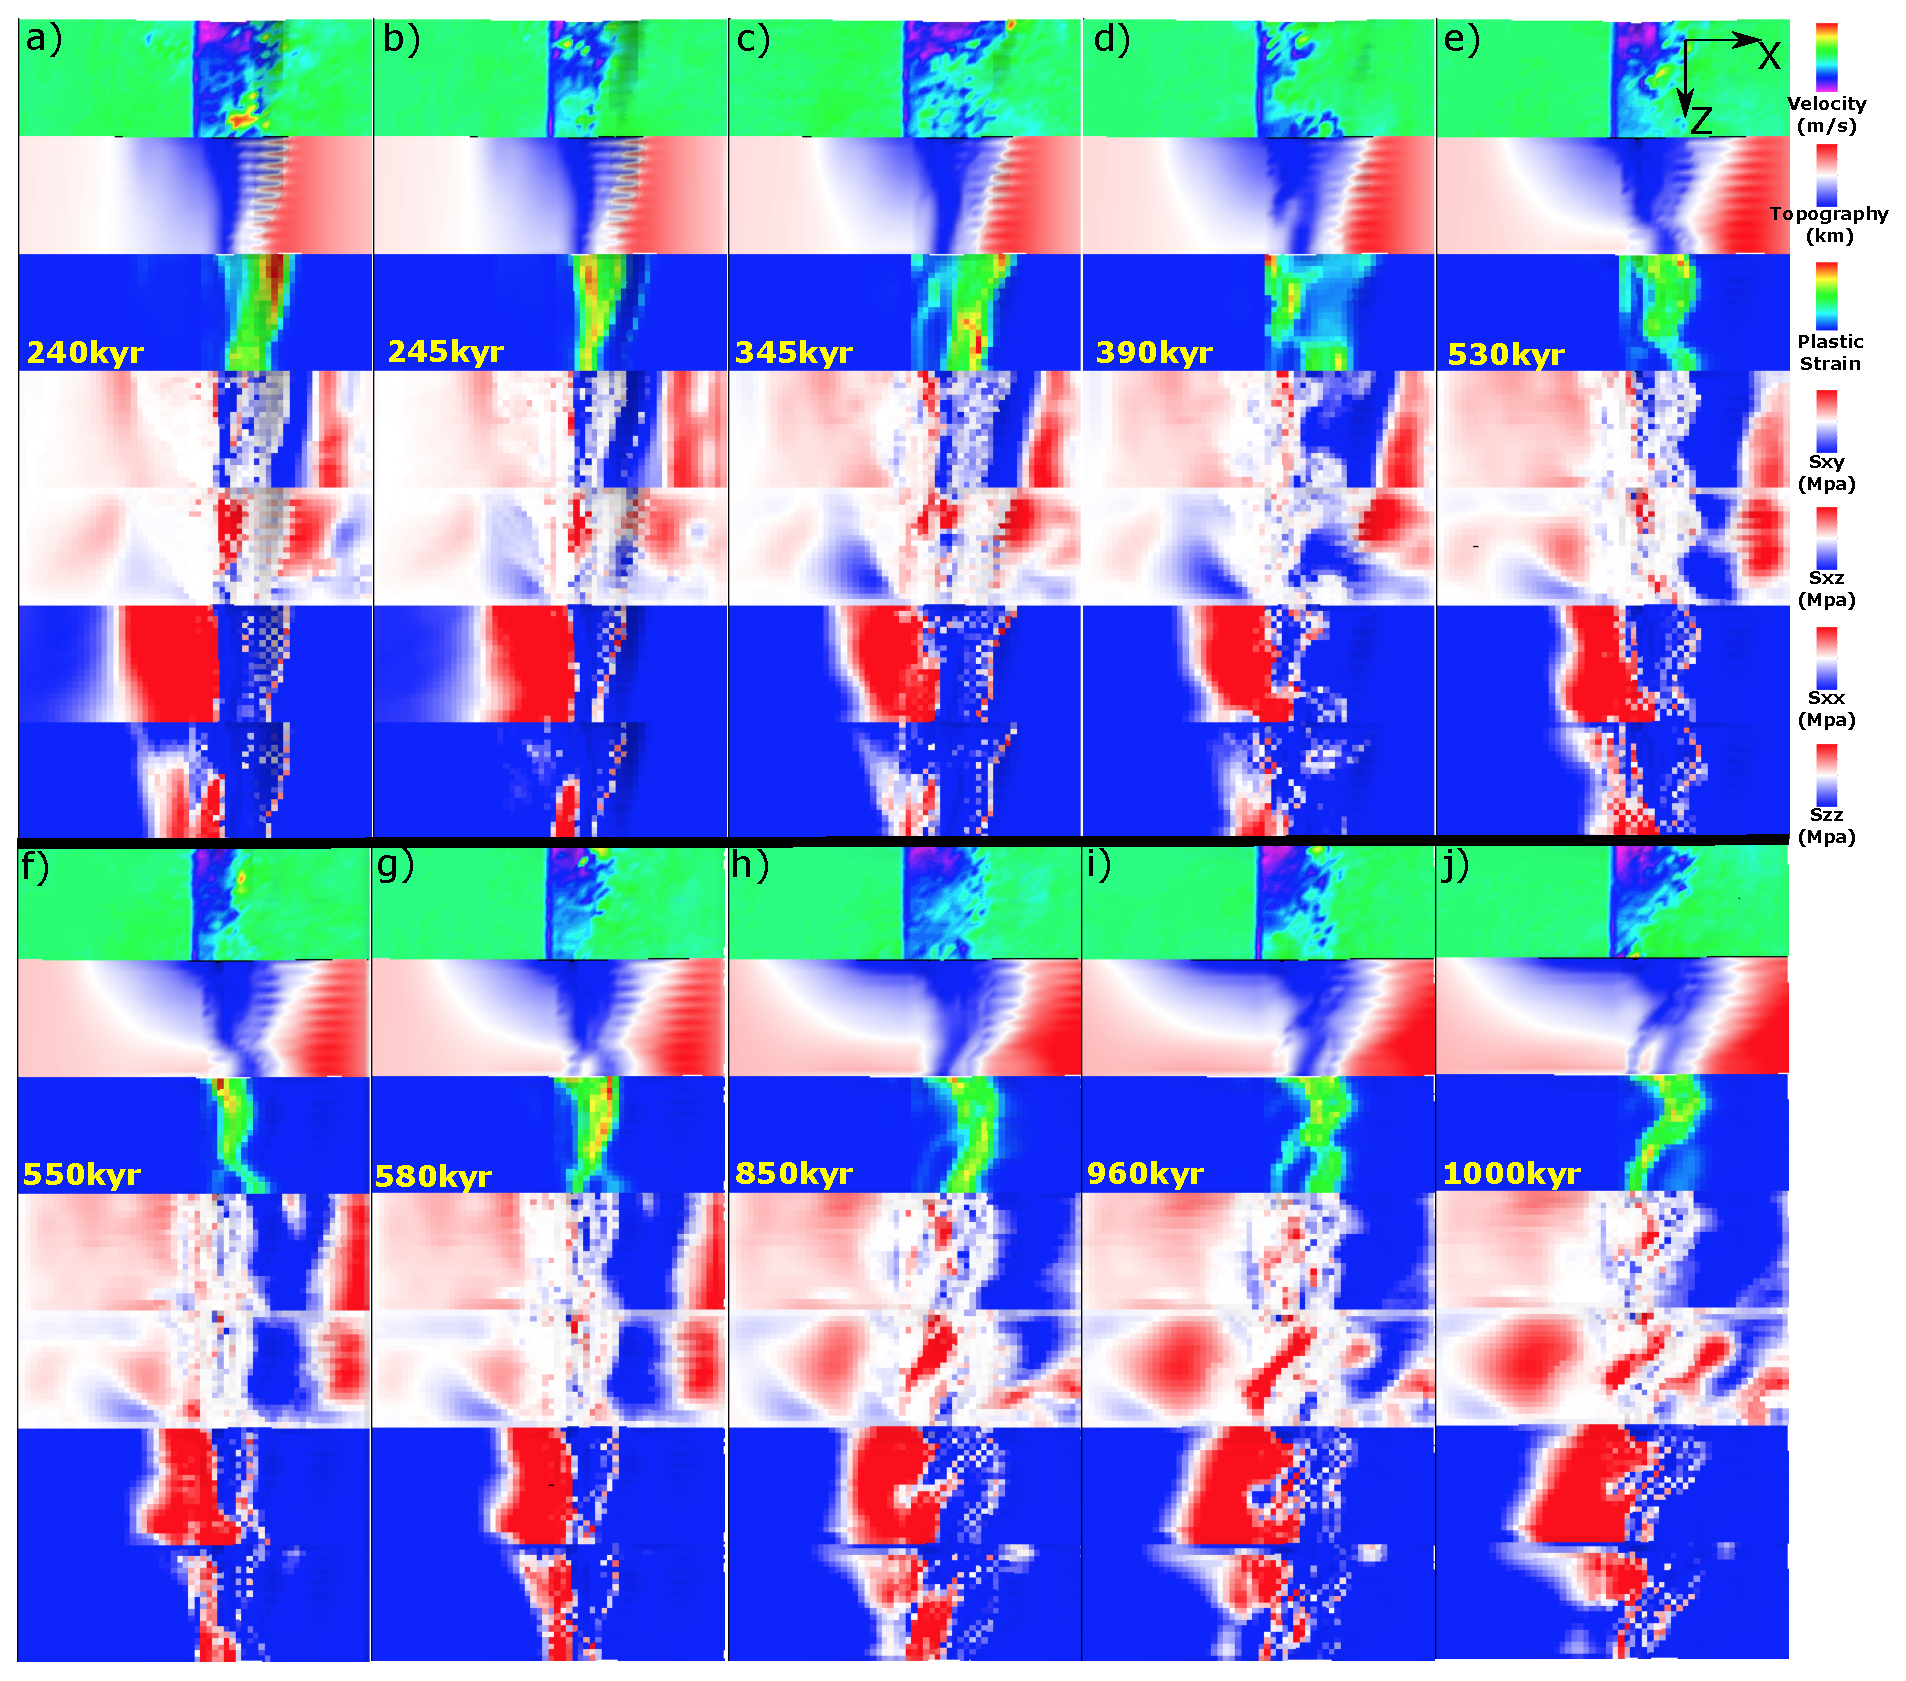
\includegraphics[width=1.0\textwidth]{./Figures/fig_Results_Weakening_5_M58SinT1_time_evolution.eps}
 \caption{Bird's-eye view of faulting and stresses evolution of M58SinT1.}
\label{fig_Results_Weakenging_5}
\end{figure}

By 240 kyr (Figure~\hyperref[fig_Results_Weakenging_5]{\ref{fig_Results_Weakenging_5}.a}), due to fast weakening (type 1), cohesion along the termination is low. Stress $\sigma_{zz}$ takes the advantage and generates $\sim$2 km wavelength corrugations parallel to the spreading direction as the termination moves further away from the ridge axis. Between 240 kyr (Figure~\hyperref[fig_Results_Weakenging_5]{\ref{fig_Results_Weakenging_5}.a}) and 245 kyr (Figure~\hyperref[fig_Results_Weakenging_5]{\ref{fig_Results_Weakenging_5}.b}), a mass wasting happens at the lower M side. The termination recedes toward the ridge axis during the mass wasting. By 345 kyr (Figure~\hyperref[fig_Results_Weakenging_5]{\ref{fig_Results_Weakenging_5}.c}), an antithetic fault forms at the lower M side (0.5 $<$ M $<$ 0.5469) with an inward fault jump happening at ridge segment with M $\in$ (0.5927, 0.6763) (Figure~\hyperref[fig_Results_3_4_2_3D_Antithetic_fault]{\ref{fig_Results_3_4_2_3D_Antithetic_fault}}). 45 kyr later, the two weak zones break through and connect to each other and take the place of the initial detachment fault at the lower M side (Figure~\hyperref[fig_Results_Weakenging_5]{\ref{fig_Results_Weakenging_5}.d}). Due to this inward fault jump, a sinistral $\sigma_{xz}$ zone (blue area in the $\sigma_{xz}$ panel) forms and is bounded by the termination of the inward fault jump near the ridge axis at the lower M side and the termination of the initial detachment fault at the higher M side. By 530 kyr (Figure~\hyperref[fig_Results_Weakenging_5]{\ref{fig_Results_Weakenging_5}.e}), the termination of the inward fault jump at the lower M side evolves to a curve with its center moving further away from the ridge axis because the inward fault jump initiates at the center and the new fault starts slipping earlier. However, the lower M side of the curve remains closer to the ridge axis due to the antithetic fault and the other end of the curve is also closer to the ridge axis because the fault initiates later. This curved termination at the lower M side also connects to the initial detachment fault at the higher M side which is further away from the ridge axis. Together, the curved termination is like a mirror reflected letter ``S''. This flipped ``S'' shape termination is also shown in topography. As the curved termination at the higher M side lasts for $\sim$300 kyr since $\sim$390 kyr, following the shape, a $\sim$10 km in wavelength and $\sim$7 km in along spreading direcion mullion structure is formed (Figure~\hyperref[fig_Results_3_4_2_M58SinT1_mullion_riderBlock_inwardFaultJump]{\ref{fig_Results_3_4_2_M58SinT1_mullion_riderBlock_inwardFaultJump}}). By $\sim$680 kyr, an inward fault jump hapens at the higher M side (0.7853 $<$ M $<$ 0.7991). It perturbs the curved shape termination and ceases the further exhumation of the mullion structure. This inward fault jump also produces a rider block that covers the inactive detachment fault and moves off axis following the exhuming footwall of the inward jumped fault.

\begin{figure}[h]
 \centering
  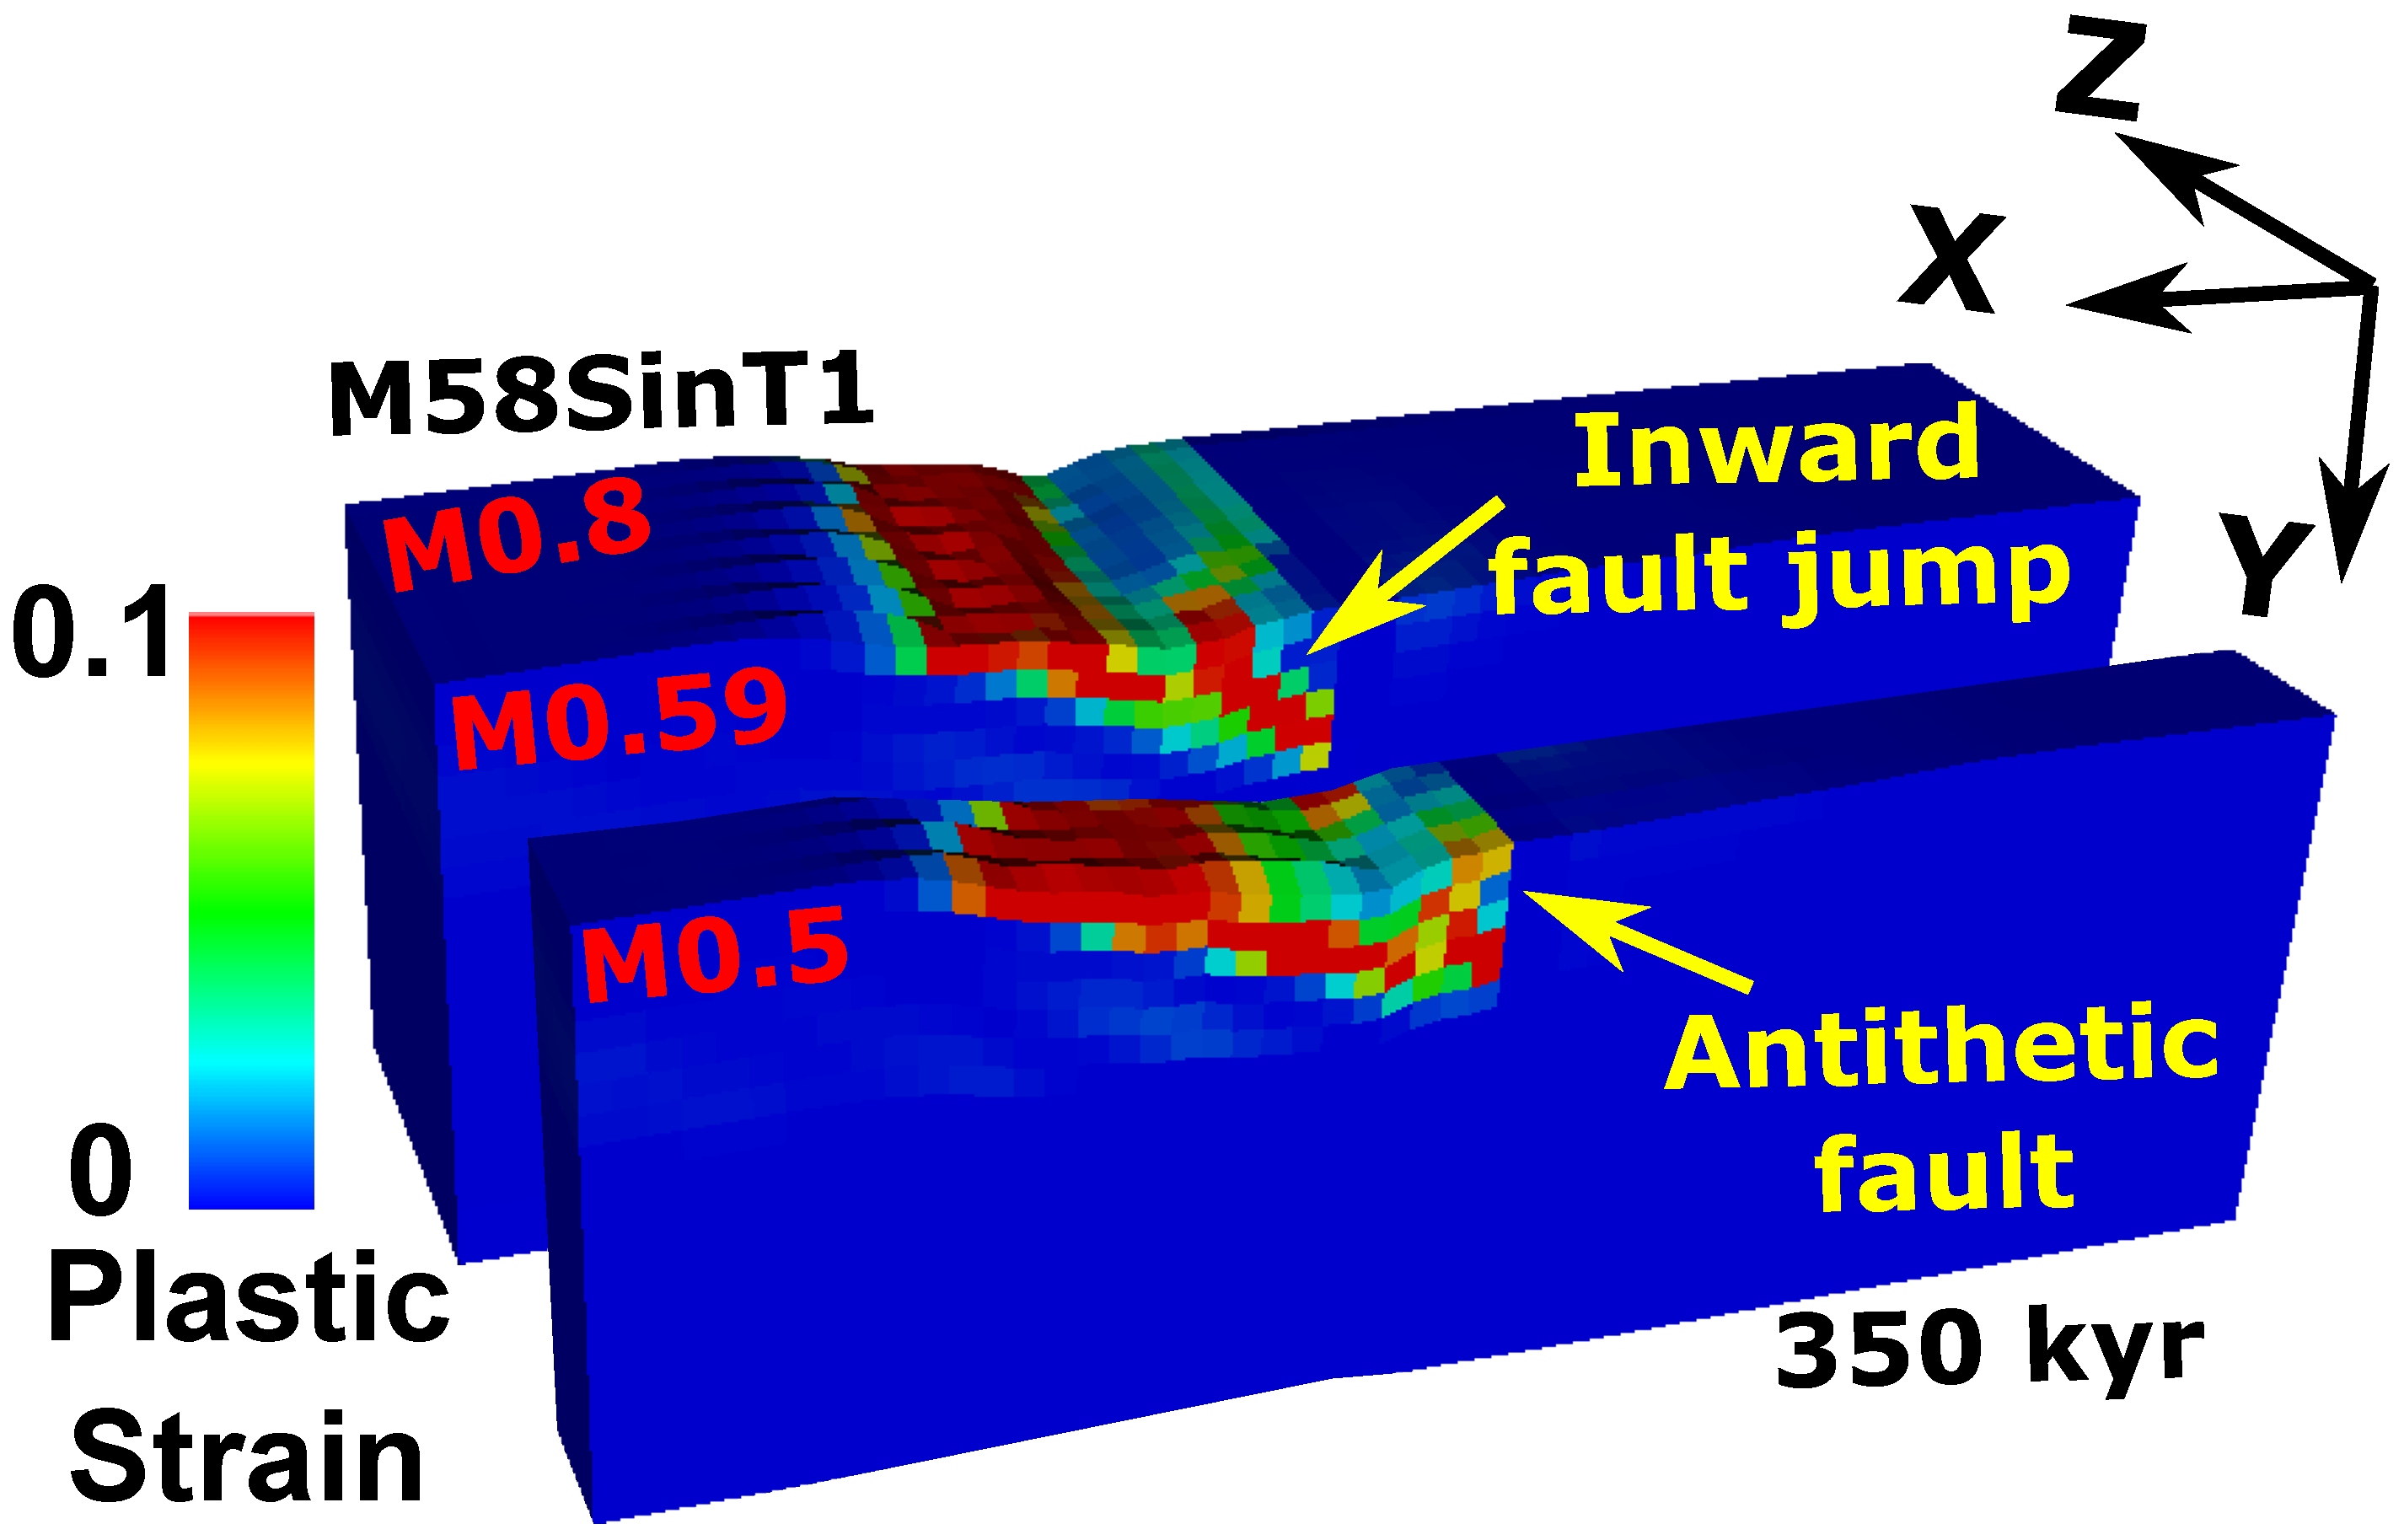
\includegraphics[width=0.6\textwidth]{./Figures/fig_Results_3_4_2_3D_Antithetic_fault.eps}
 \caption{Plastic strain for M58SinT1 at 350 kyr.}
\label{fig_Results_3_4_2_3D_Antithetic_fault}
\end{figure}

\begin{figure}[h]
 \centering
  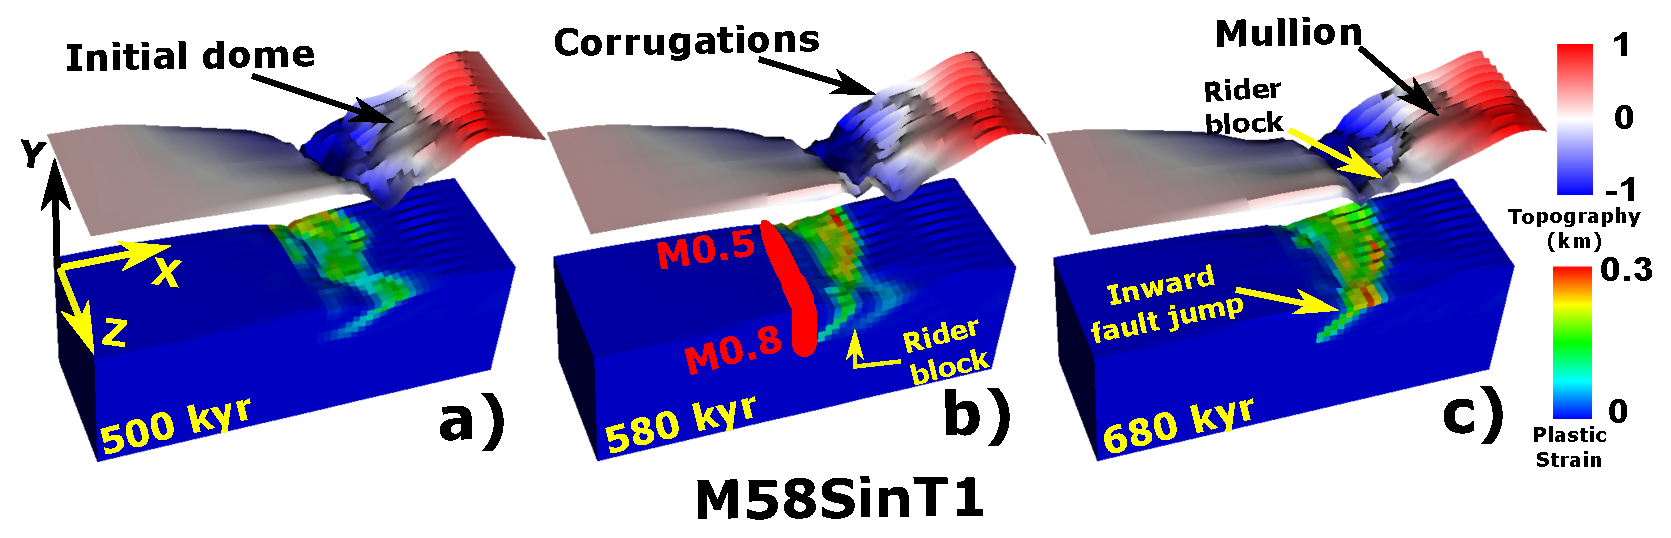
\includegraphics[width=1.0\textwidth]{./Figures/fig_Results_3_4_2_M58SinT1_mullion_riderBlock_inwardFaultJump.eps}
 \caption{Evolution of faulting and morphologies of M58SinT1.}
\label{fig_Results_3_4_2_M58SinT1_mullion_riderBlock_inwardFaultJump}
\end{figure}

Between 530 kyr (Figure~\hyperref[fig_Results_Weakenging_5]{\ref{fig_Results_Weakenging_5}.e}) and 550 kyr (Figure~\hyperref[fig_Results_Weakenging_5]{\ref{fig_Results_Weakenging_5}.f}), another mass wasting happens at the lower M side (0.5 $<$ M $<$ 0.5469) where a slump block with a surface area of $\sim$9 km$^{2}$ flows down the topography slope into the trough. Termination recedes backward to the ridge axis. By 580 kyr, termination at the lower M side moves further away from the ridge axis due to less magma supply. Between 580 kyr and 850 kyr, due to two antithetic faults at the lower M side (M $\in$ (0.5, 0.5469) $\cup$ (0.5927, 0.6567)), the termination at the lower M side recedes and the previous mirror reflected ``S'' shape termination evolves to a half circle curve (Figure~\hyperref[fig_Results_Weakenging_5]{\ref{fig_Results_Weakenging_5}.h}). The shape is also reflected in the topography. By 960 kyr (Figure~\hyperref[fig_Results_Weakenging_5]{\ref{fig_Results_Weakenging_5}.i})), at the ridge segment with M $\in$ (0.6763, 0.7121), another inward fault jump replaces the detachment fault away from the ridge axis and retreats the termination backward to the ridge axis forming two half circle curves with wavelengths of around half of the model domain in $z$-axis. A large dextral shear zone (red region $\sim$40 $\degree$ oblique to ridge axis) is seen in the $\sigma_{xz}$ panel. The shear stress $\sigma_{xz}$ is produced by the inward fault jump at the center of the ridge segment that previous hanging wall changes to the footwall of the inward jumped fault and generates an offset between the old hangingwall at the lower M end and the new footwall of the inward jumped fault. By 1000 kyr, due to the along ridge coupling, the inward fault jump propogates to the end of the high M side (Figure~\hyperref[fig_Results_Weakenging_5]{\ref{fig_Results_Weakenging_5}.j}). 

\paragraph{M58SinT2}\label{para_M58SinT2}
~\\
As shown in Figure~\hyperref[fig_Results_Weakenging_6]{\ref{fig_Results_Weakenging_6}}, a fault initiates on the left-hand side of the ridge axis (Figure~\hyperref[fig_Results_Weakenging_6]{\ref{fig_Results_Weakenging_6}.a}). The breakaway at the lower M side moves away from the ridge axis further than that of the higher M side. It takes longer time of $\sim$100 kyr to form a localized fault plane through the whole ridge segment due to the slower rate of weakening (type 2). By 215 kyr (Figure~\hyperref[fig_Results_Weakenging_6]{\ref{fig_Results_Weakenging_6}.b}), fault alternates to the conjugate plate and gradually replaces the initial one. Corrugations are only produced at the lower M side (M $\in$ (0.5, 0.6763)). By 330 kyr, fault alternates again. Between 490 kyr (Figure~\hyperref[fig_Results_Weakenging_6]{\ref{fig_Results_Weakenging_6}.d}) and 495 kyr (Figure~\hyperref[fig_Results_Weakenging_6]{\ref{fig_Results_Weakenging_6}.e}), a mass wasting happens with termination receding. A slump block with an area of $\sim$16 km$^{2}$ flows down the topography slope into the trough. With fault alternation, the shape of the median valley is no longer a typical hourglass. However, at the lower M side, the median valley is still wider and deeper. Smaller wavelength abyssal hills are produced at the higher M side. %In addition, M58SinT2 has a fault alternation frequency of $\sim$150 kyr which is higher than that of M88ConT2. \add[XT]{Reason for this difference needs further discussion.}

\begin{figure}[h]
 \centering
  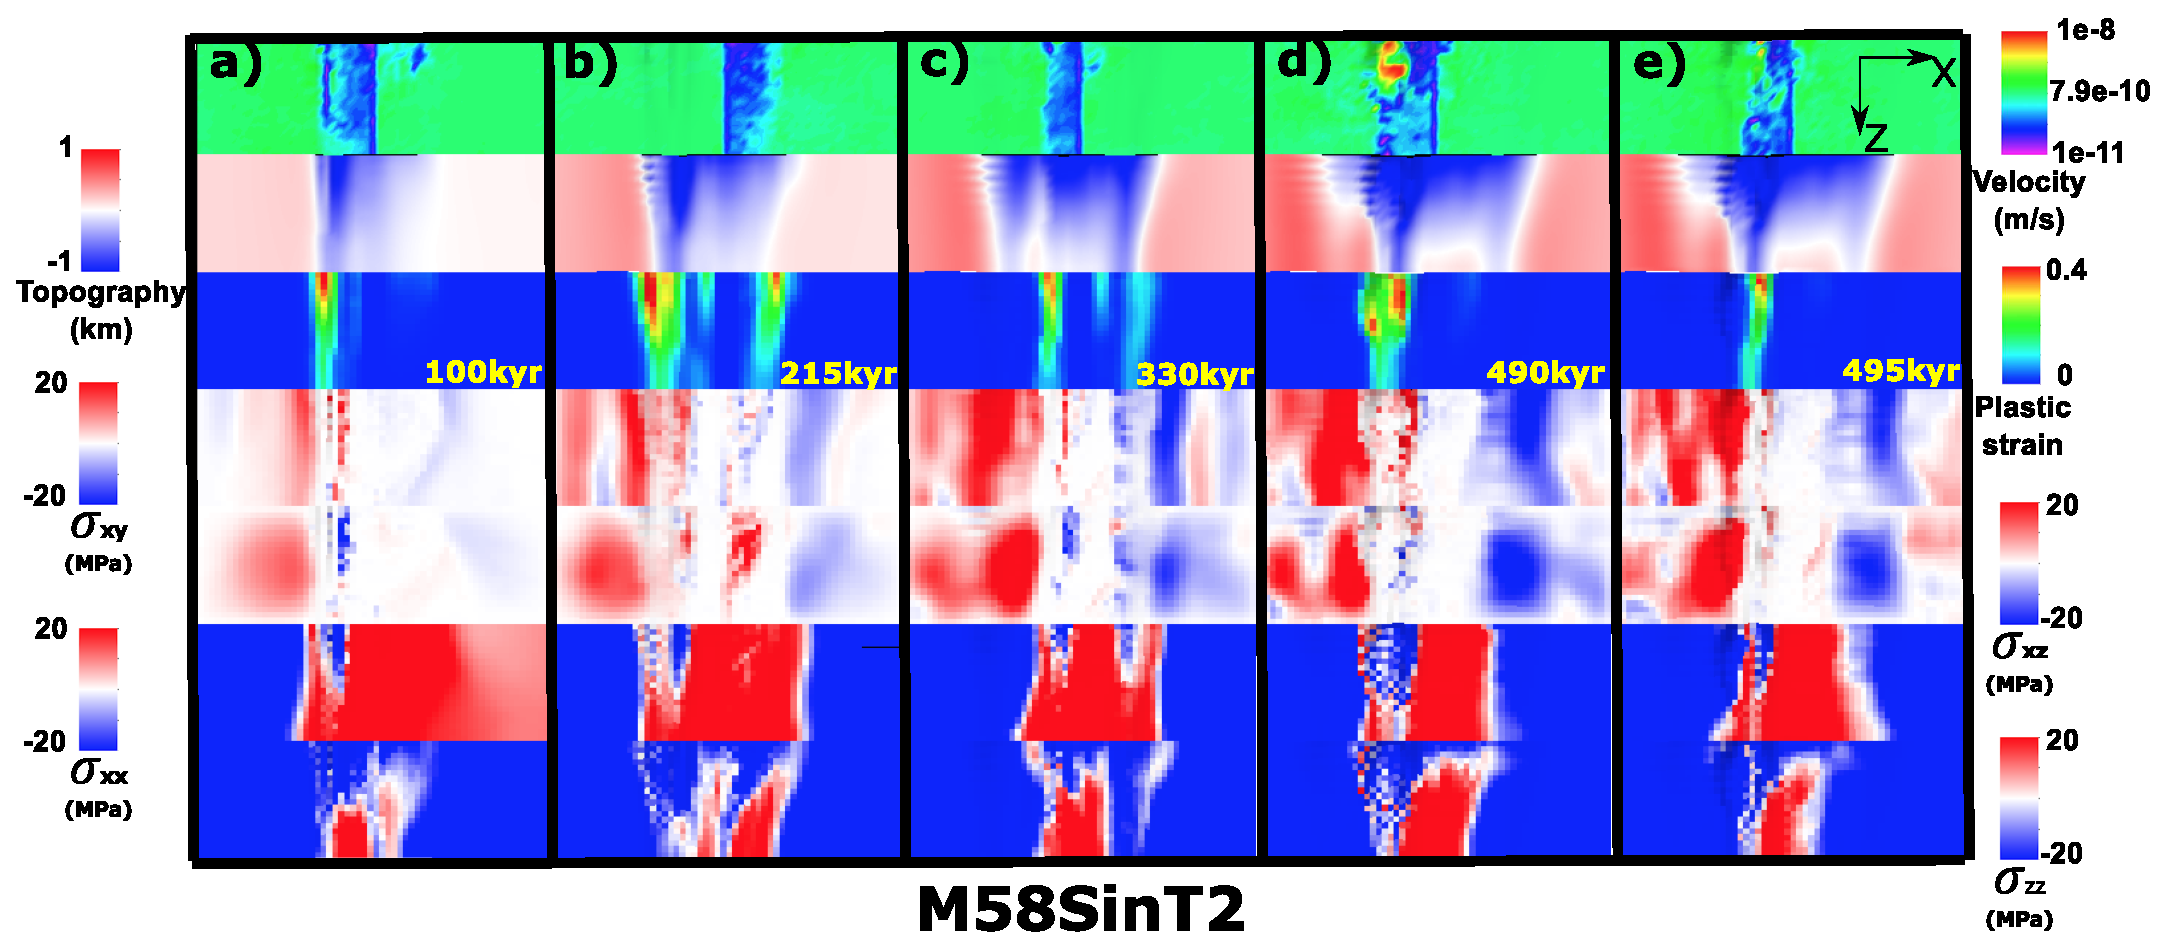
\includegraphics[width=1.0\textwidth]{./Figures/fig_Results_Weakening_6_M58SinT2_time_evolution.eps}
 \caption{Bird's-eye view of faulting and stresses evolution of M58SinT2.}
\label{fig_Results_Weakenging_6}
\end{figure}

\subsubsection{M58SqrtT1 versus M58SqrtT2}

The major difference between M58SqrtT1 and M58SqrtT2 is also whether the normal fault alternates or not.

\paragraph{M58SqrtT1}\label{para_M58SqrtT1}
~\\
By 260 kyr, breakaway at M $=$ 0.5 moves $\sim$5 km further away from the ridge axis than that at the higher M end (Figure~\hyperref[fig_Results_Weakenging_7]{\ref{fig_Results_Weakenging_7}.a}). Corrugations with a wavelength of $\sim$2 km are produced along the ridge. By 370 kyr (Figure~\hyperref[fig_Results_Weakenging_7]{\ref{fig_Results_Weakenging_7}.b}), due to larger value of $\frac{\partial M}{\partial Z}$ at the lower M side, a vertical tensile failure takes place at M $\in$ (0.5, 0.5949). Two parallel sinistral shear stress zones (blue) are seen in the $\sigma_{xz}$ panel. By 400 kyr (Figure~\hyperref[fig_Results_Weakenging_7]{\ref{fig_Results_Weakenging_7}.c}), an inward fault jump happens where M $\in$ (0.5949, 0.7121) and it propagates to the end of the higher M side and replaces the initial detachment fault at the higher M side by 460 kyr (Figure~\hyperref[fig_Results_Weakenging_7]{\ref{fig_Results_Weakenging_7}.d}). By 590 kyr (Figure~\hyperref[fig_Results_Weakenging_7]{\ref{fig_Results_Weakenging_7}.e}), an inward fault jump happens at the lower M side (M $<$ 0.5949) and connect with the normal fault at the higher M side replacing the initial detachment fault. An $\sim$18 km$^{2}$ triangular shape (bird's-eye view) rider block is produced at the lower M side. Termination at the center of the ridge segment moves the furthest away from the ridge axis. This is because the previous inward fault jump first initiates there and starts slipping earlier. It is also because the value of M is lower at the segment center than the higher M end. By 660 kyr (Figure~\hyperref[fig_Results_Weakenging_7]{\ref{fig_Results_Weakenging_7}.f}), as the previous inward jumped fault at the higher M side evolves, another dome is produced. There is a hint of high angle normal fault at the region with M $<$ 0.5949 on the conjugate plate. But it doesn't develop. By 730 kyr (Figure~\hyperref[fig_Results_Weakenging_7]{\ref{fig_Results_Weakenging_7}.g}, the termination evolves to a ``half circle'' and the shape is also seen in the topography. By 780 kyr (Figure~\hyperref[fig_Results_Weakenging_7]{\ref{fig_Results_Weakenging_7}.h}), another inward fault jump appears at the ridge segment with M $\in$ (0.6342, 0.7121) and produced a curved termination with a wavelenth of $\sim$10 km. It has the potential to create a large wavelength mullion structure. Meanwhile, at the lower M side (M $<$ 0.5949) near the ridge axis, an antithetic fault forms and propagates toward the higher M side (Figure~\hyperref[fig_Results_Weakenging_7]{\ref{fig_Results_Weakenging_7}.i}). It triggers another inward fault jump at the lower M side and produces another rider block. The inward jumped fault later connects with the detachment fault at the higher M side (Figure~\hyperref[fig_Results_Weakenging_7]{\ref{fig_Results_Weakenging_7}.j}). In addition, a tensile failure shows its hint at the lower M side (M $<$ 0.6342) of the conjugate plate.

\begin{figure}[h]
 \centering
  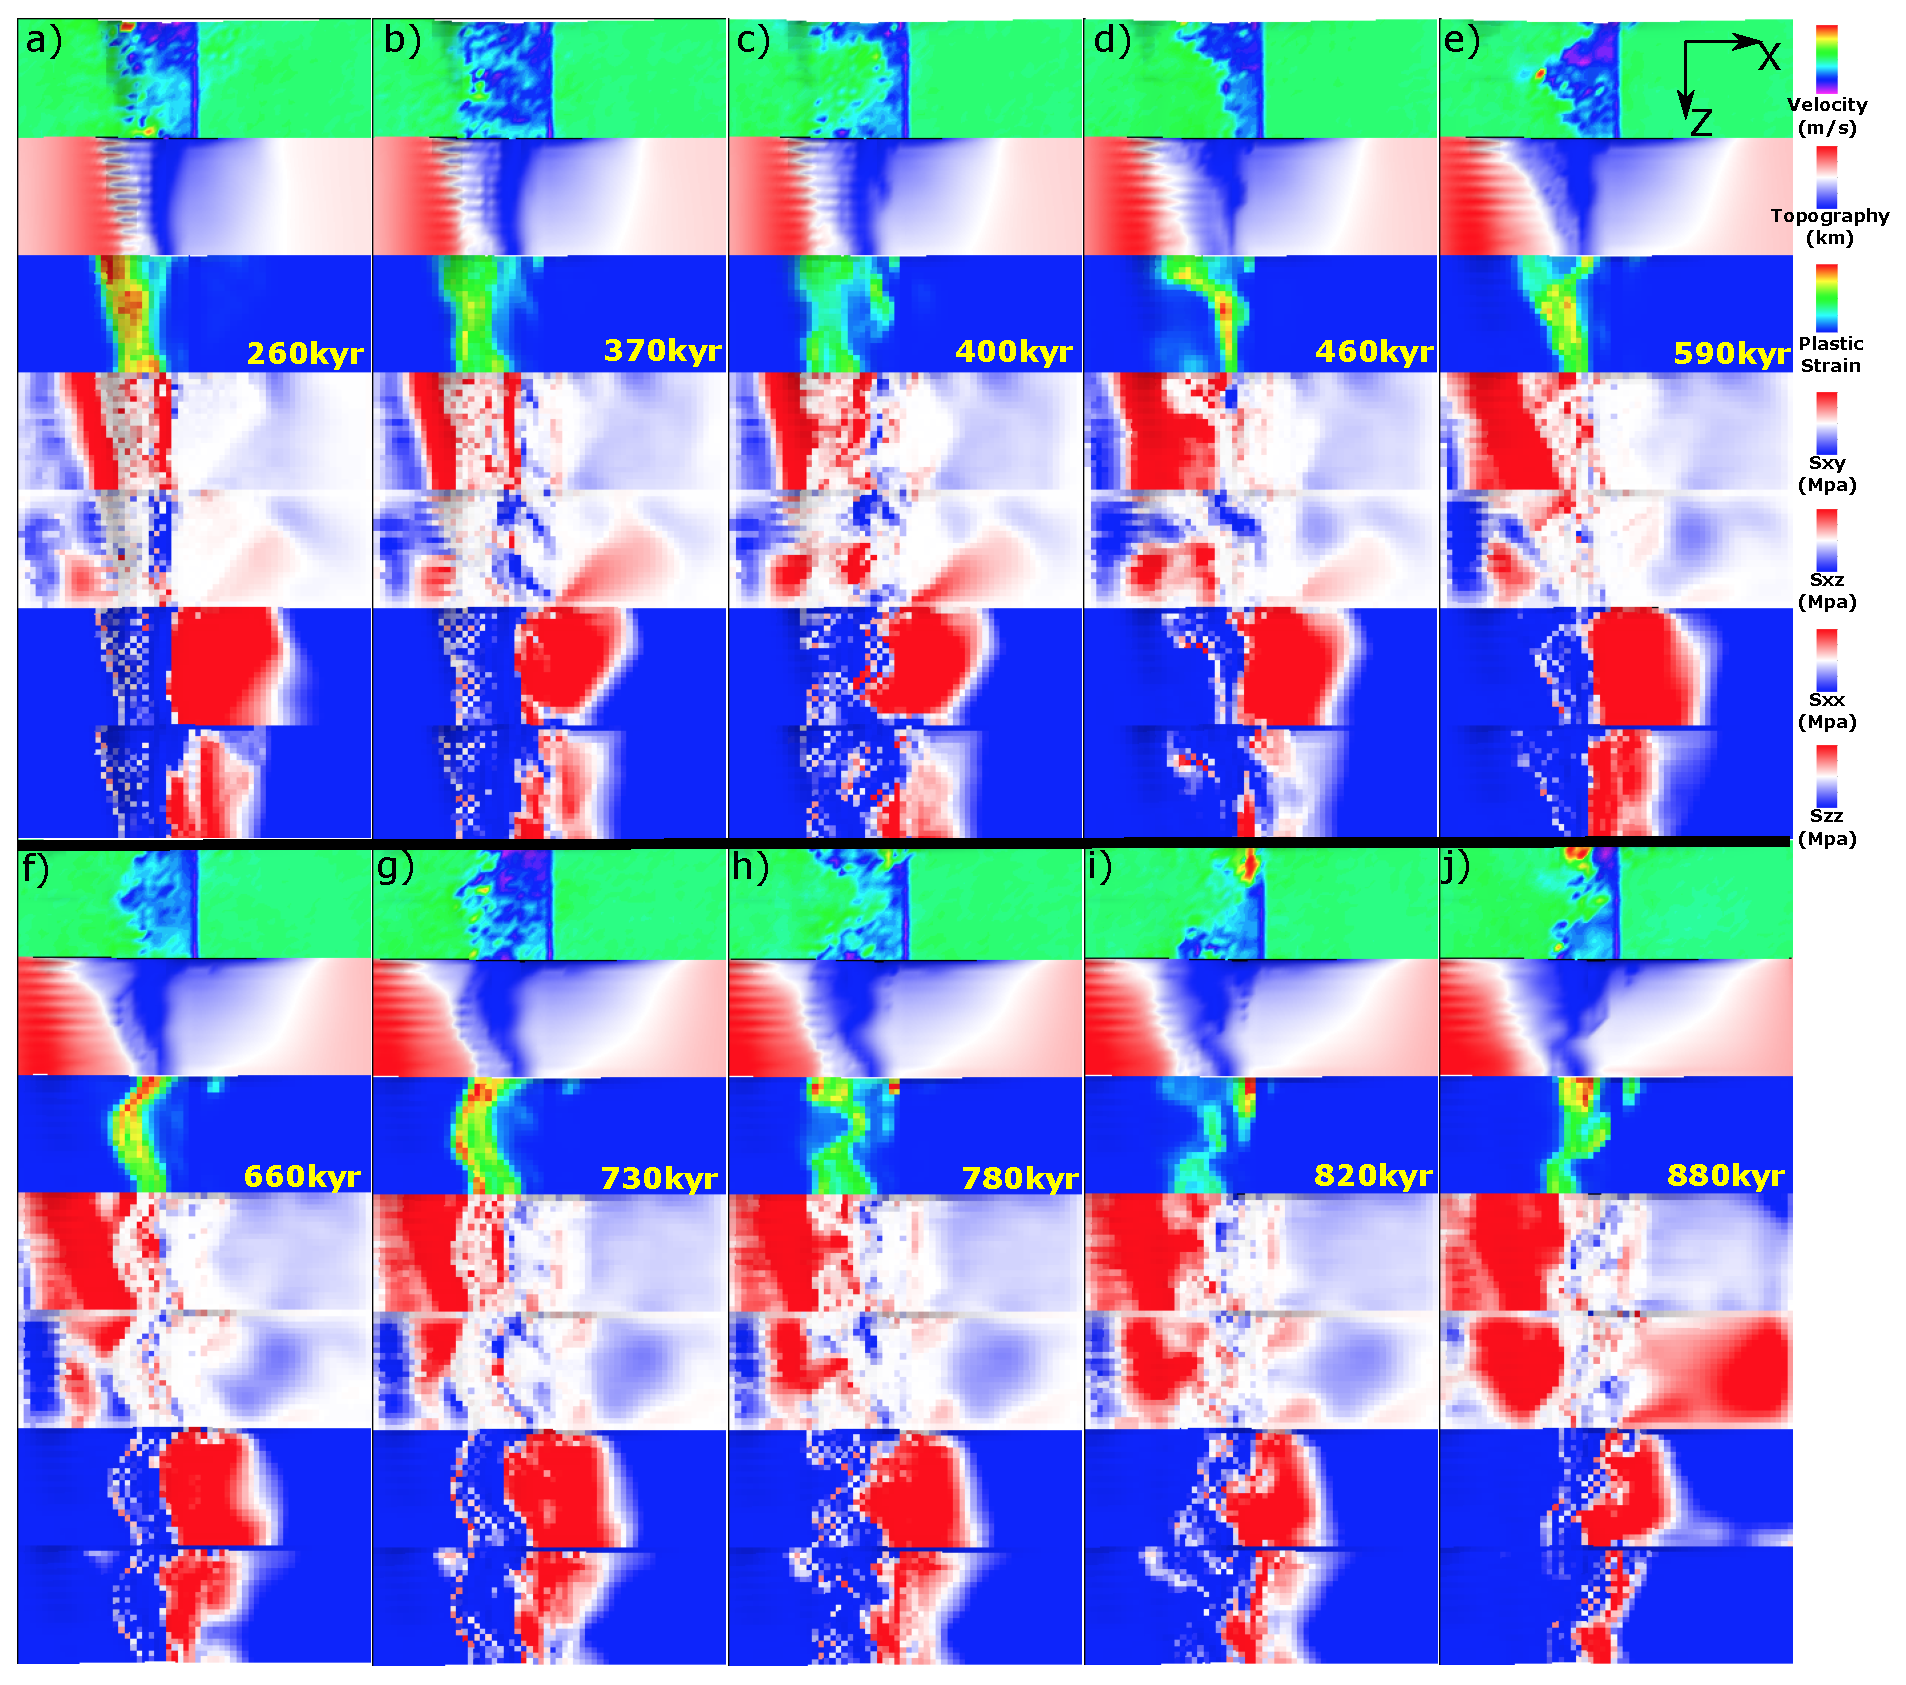
\includegraphics[width=1.0\textwidth]{./Figures/fig_Results_Weakening_7_M58SqrtT1_time_evolution.eps}
 \caption{Bird's-eye view of faulting and stresses evolution of M58SqrtT1.}
\label{fig_Results_Weakenging_7}
\end{figure}

\vspace{1.5cm}
\paragraph{M58SqrtT2}\label{para_M58SqrtT2}
~\\
By 195 kyr (Figure~\hyperref[fig_Results_Weakenging_8]{\ref{fig_Results_Weakenging_8}.a}), breakaway at the lower M side moves further away from the ridge axis. Three corrugations begin to show up due to isochron-parallel tensile failure. Median valley on the conjugate plate is wider at the lower M side because less magma supply results in larger amount of elastic depression. Between 195 kyr (Figure~\hyperref[fig_Results_Weakenging_8]{\ref{fig_Results_Weakenging_8}.a}) and 200 kyr (Figure~\hyperref[fig_Results_Weakenging_8]{\ref{fig_Results_Weakenging_8}.b}), mass wasting happens along the ridge and is followed by the termination retreat. By 270 kyr fault alternates (Figure~\hyperref[fig_Results_Weakenging_8]{\ref{fig_Results_Weakenging_8}.c}). The shape of the alternated fault follows the curved shape shear $\sigma_{xy}$ zone (red) as seen since $\sim$195 kyr on the left-hand side of the ridge axis. By 330 kyr (Figure~\hyperref[fig_Results_Weakenging_8]{\ref{fig_Results_Weakenging_8}.d}), at the lower M side, an inward fault jump happens and takes the place of the old fault further away from the ridge axis. By 460 kyr (Figure~\hyperref[fig_Results_Weakenging_8]{\ref{fig_Results_Weakenging_8}.e}), fault alternates again to the right hand side of the ridge axis.

\begin{figure}[h]
 \centering
  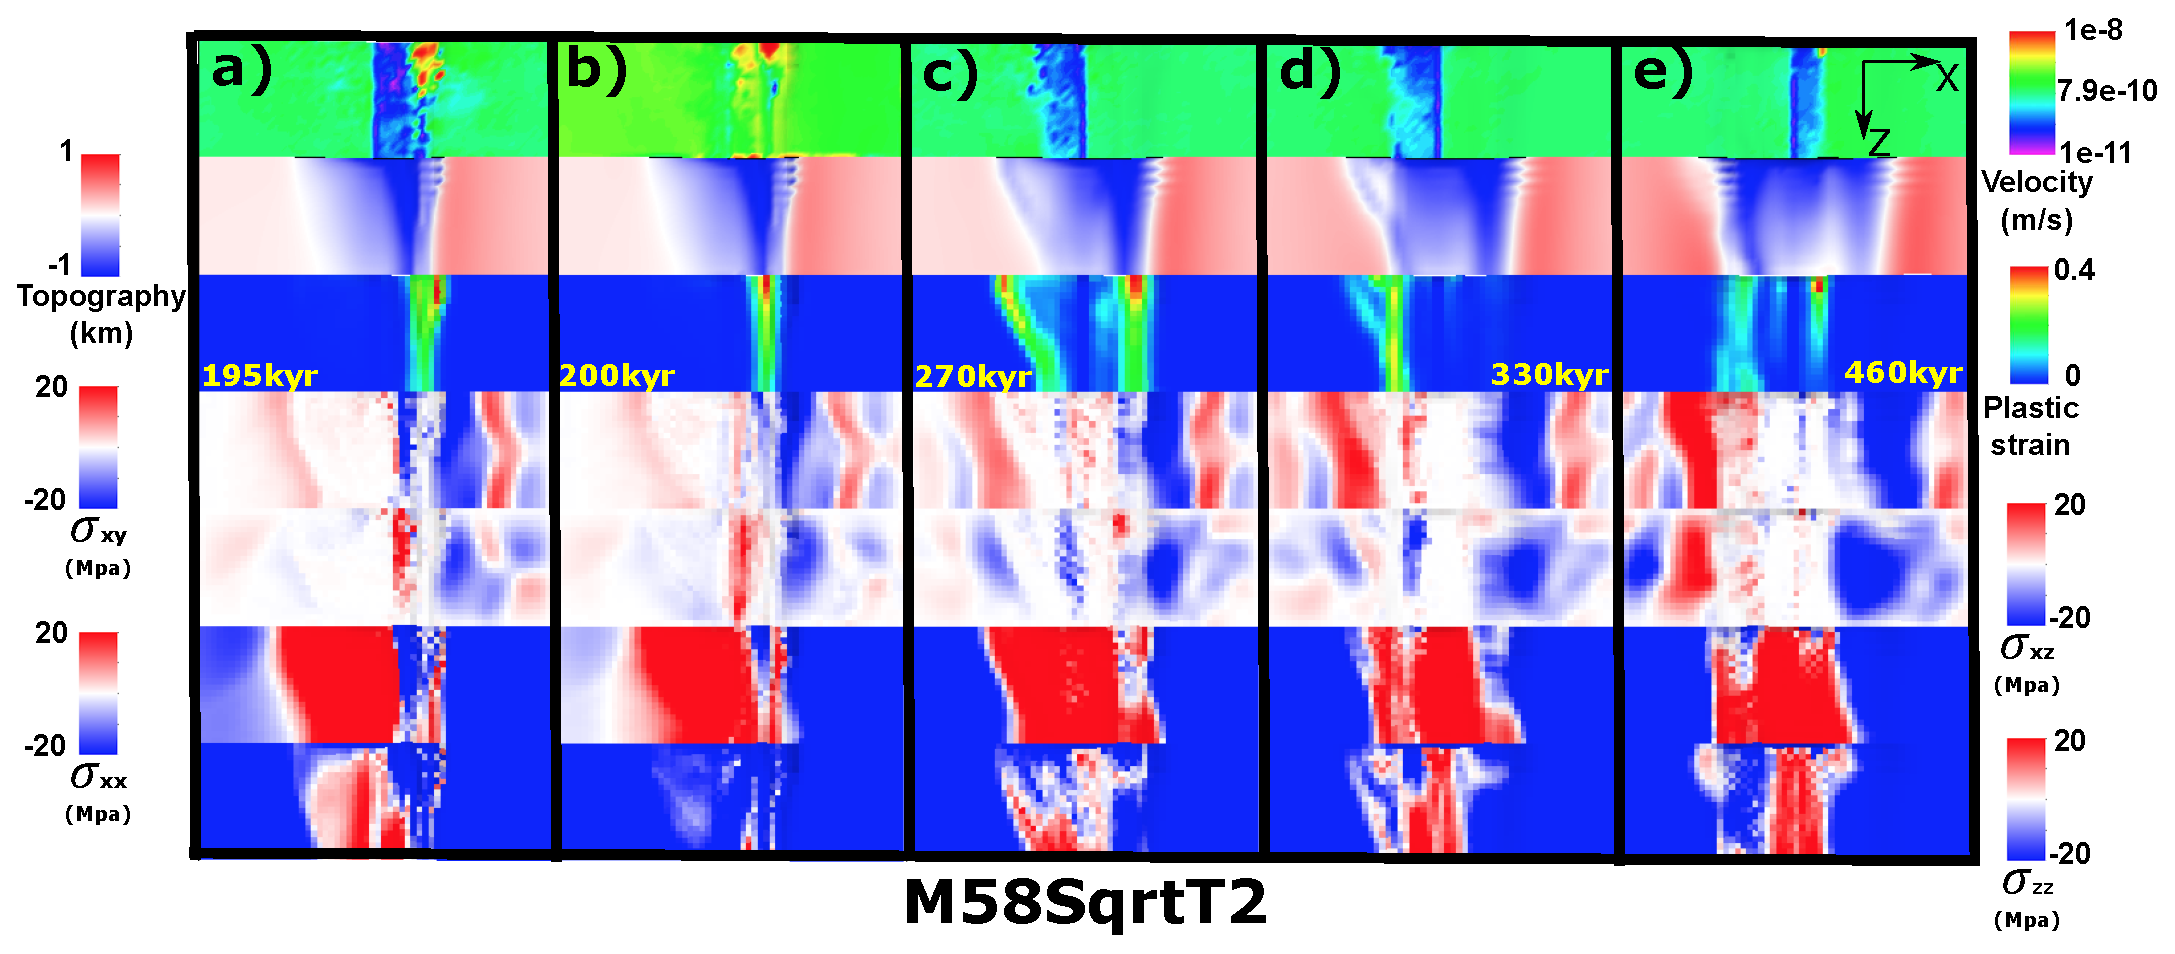
\includegraphics[width=1.0\textwidth]{./Figures/fig_Results_Weakening_8_M58SqrtT2_time_evolution.eps}
 \caption{Faulting and stresses evolution for M58SqrtT2.}
\label{fig_Results_Weakenging_8}
\end{figure}

\subsection{Effects of the range of M variation}
Generally, M57 and M58 models create a median valley much narrower and shallower than that of M28 models.

\subsubsection{SinT1}

\paragraph{M57SinT1 versus M58SinT1}\label{M57SinT1 versus M58SinT1}

~\\
For description of M57SinT1 evolution with respect to time, please refer to Section~\hyperref[para_M57SinT1]{\ref{para_M57SinT1}} and Figure~\hyperref[fig_Results_Weakenging_3]{\ref{fig_Results_Weakenging_3}}. For description of M58SinT1 evolution with respect to time, please refer to  Section~\hyperref[para_M58SinT1]{\ref{para_M58SinT1}} and Figure~\hyperref[fig_Results_Weakenging_5]{\ref{fig_Results_Weakenging_5}}. Comparing M57SinT1 and M58SinT1, the major difference is that the faulting pattern evolution for M58SinT1 is much more dynamic with a higher frequency of inward fault jumps, mass wasting and connection of the offsetted fault zones. For M58SinT1, the inward fault jumps and antithetic faults usually replace the old ones. However, for M57SinT1, diking is not robust enough to create big enough stress perturbation along the ridge axis for inward fault jumps or antithetic faults to take the place of the original one. At the lower M side, antithetic faults only help to accommodate tensional stress which assists in maintaining a termination near the ridge axis while the termination at the higher M side gradually moves off axis. This produces an OCC with larger dome at the lower M side than higher M side which is opposite to the shape of the OCC produced by M58SinT1. 

\paragraph{M28SinT1}\label{para_M28SinT1}
~\\
As shown in Figure~\hyperref[fig_Results_MRange_1]{\ref{fig_Results_MRange_1}}, faulting evolution is much less dynamic than that of M58SinT1. One detachment fault keeps active on the right hand side of the ridge axis. Only inward fault jump happens $\sim$540 kyr (Figure~\hyperref[fig_Results_MRange_1]{\ref{fig_Results_MRange_1}.d}). By $\sim$100 kyr (Figure~\hyperref[fig_Results_MRange_1]{\ref{fig_Results_MRange_1}.a}), breakaway at the lower M side moves $\sim$4 km further away from ridge axis than the higher M side. By 250 kyr (Figure~\hyperref[fig_Results_MRange_1]{\ref{fig_Results_MRange_1}.b}), $\sim$4 corrugations begin to evolve at the lower M side (M $\in$ (0.2, 0.5135)). By 420 kyr, at the higher M side, a hint of inward fault jump begins to show up. It delvelops into an inward fault jump by 540 kyr (Figure~\hyperref[fig_Results_MRange_1]{\ref{fig_Results_MRange_1}.d}) and propagates toward higher M side. At the lower M side (M $\in$ (0.2, 0.2939)), a tensile failure takes up part of the plate extension and helps maintain a closer to ridge axis termination than the moving termination at the region with M $\in$ (0.4724, 0.6562) (Figure~\hyperref[fig_Results_MRange_1]{\ref{fig_Results_MRange_1}.e}). The curved toward ridge axis termination at the lower M side produces a mullion structure.

\begin{figure}[h]
 \centering
  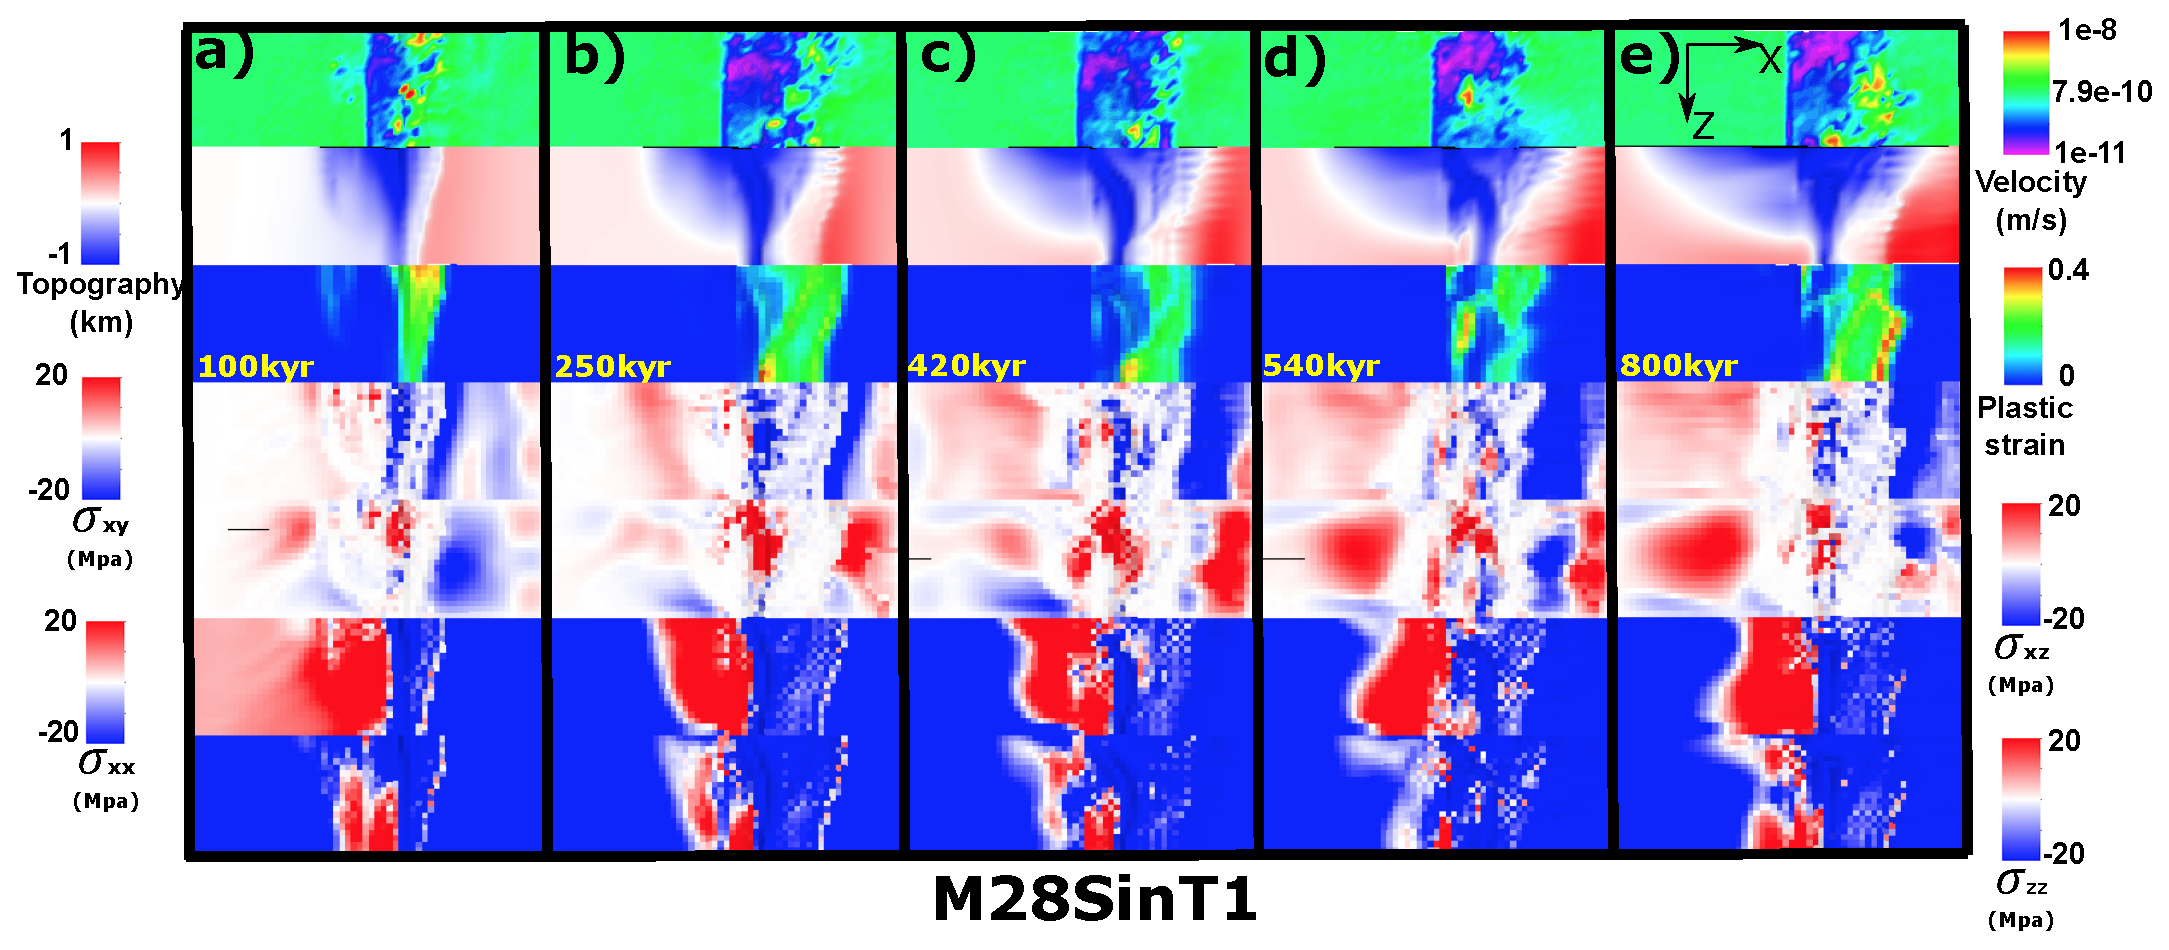
\includegraphics[width=1.0\textwidth]{./Figures/fig_Results_MRange_1_M28SinT1_time_evolution.eps}
 \caption{M28SinT1 (Table~\hyperref[Tab1_1]{\ref{Tab1_1}}) faulting and stresses evolution with respect to time.}
\label{fig_Results_MRange_1}
\end{figure}

\subsubsection{M57SinT2 versus M58SinT2}

For description of M57SinT2 evolution with respect to time, please refer to Section~\hyperref[para_M57SinT2]{\ref{para_M57SinT2}} and Figure~\hyperref[fig_Results_Weakenging_4]{\ref{fig_Results_Weakenging_4}}. For description of M58SinT1 evolution with respect to time, please refer to Section~\hyperref[para_M58SinT2]{\ref{para_M58SinT2}} and Figure~\hyperref[fig_Results_Weakenging_6]{\ref{fig_Results_Weakenging_6}}. A major difference is that M57SinT2 has no fault alternation while M58SinT2 has.

\subsubsection{M28LinT1 versus M57LinT1}

For description of M28LinT1 evolution with respect to time, please refer to Section~\hyperref[sec_M28LinT1]{\ref{sec_M28LinT1}}.

\paragraph{M57LinT1}\label{para_M57LinT1}
~\\
As shown in Figure~\hyperref[fig_Results_MRange_2]{\ref{fig_Results_MRange_2}}, between 160 kyr (Figure~\hyperref[fig_Results_MRange_2]{\ref{fig_Results_MRange_2}.a}) and 162.5 kyr (Figure~\hyperref[fig_Results_MRange_2]{\ref{fig_Results_MRange_2}.b}), a mass wasting happens. The corrugations have a relatively high amplitude. Due to less M variation (0.2), the along ridge offset in breakaways is smaller. The median valley almost has a constant width along the ridge. By 350 kyr (Figure~\hyperref[fig_Results_MRange_2]{\ref{fig_Results_MRange_2}.c}), a tensile failure happens at the region with M $\in$ (0.5, 0.61) and generates a linear topography low. Another shorter tensile failure at the higher M side (M $>$ 0.64) helps maintain a high angle normal fault near the ridge axis. By 430 kyr (Figure~\hyperref[fig_Results_MRange_2]{\ref{fig_Results_MRange_2}.d}), the tensile failure at the lower M side (M $<$ 0.52) is responsible for the retreat of the termination. Whereas at M $\in$ (0.54, 0.59), the termination moves further away from the ridge axis. This curved termination results in a ``dog bone'' shape topography as seen at 640 kyr (Figure~\hyperref[fig_Results_MRange_2]{\ref{fig_Results_MRange_2}.e}) and is also responsible for the large sinistral shear (blue) stress $\sigma_{xz}$. By 705 kyr (Figure~\hyperref[fig_Results_MRange_2]{\ref{fig_Results_MRange_2}.f}), an inward fault jump happens and replaces the original detachment fault at the higher M side with a length of $\sim$15 km. This inward jumped fault connects with the detachment fault at the lower M side. The new ``L'' shape termination is responsible for the topography seen at 1000 kyr (Figure~\hyperref[fig_Results_MRange_2]{\ref{fig_Results_MRange_2}.h}). The termination at the higher M side soon catches up the termination at the lower M side due to the presence of a tensile failure.

\begin{figure}[h]
 \centering
  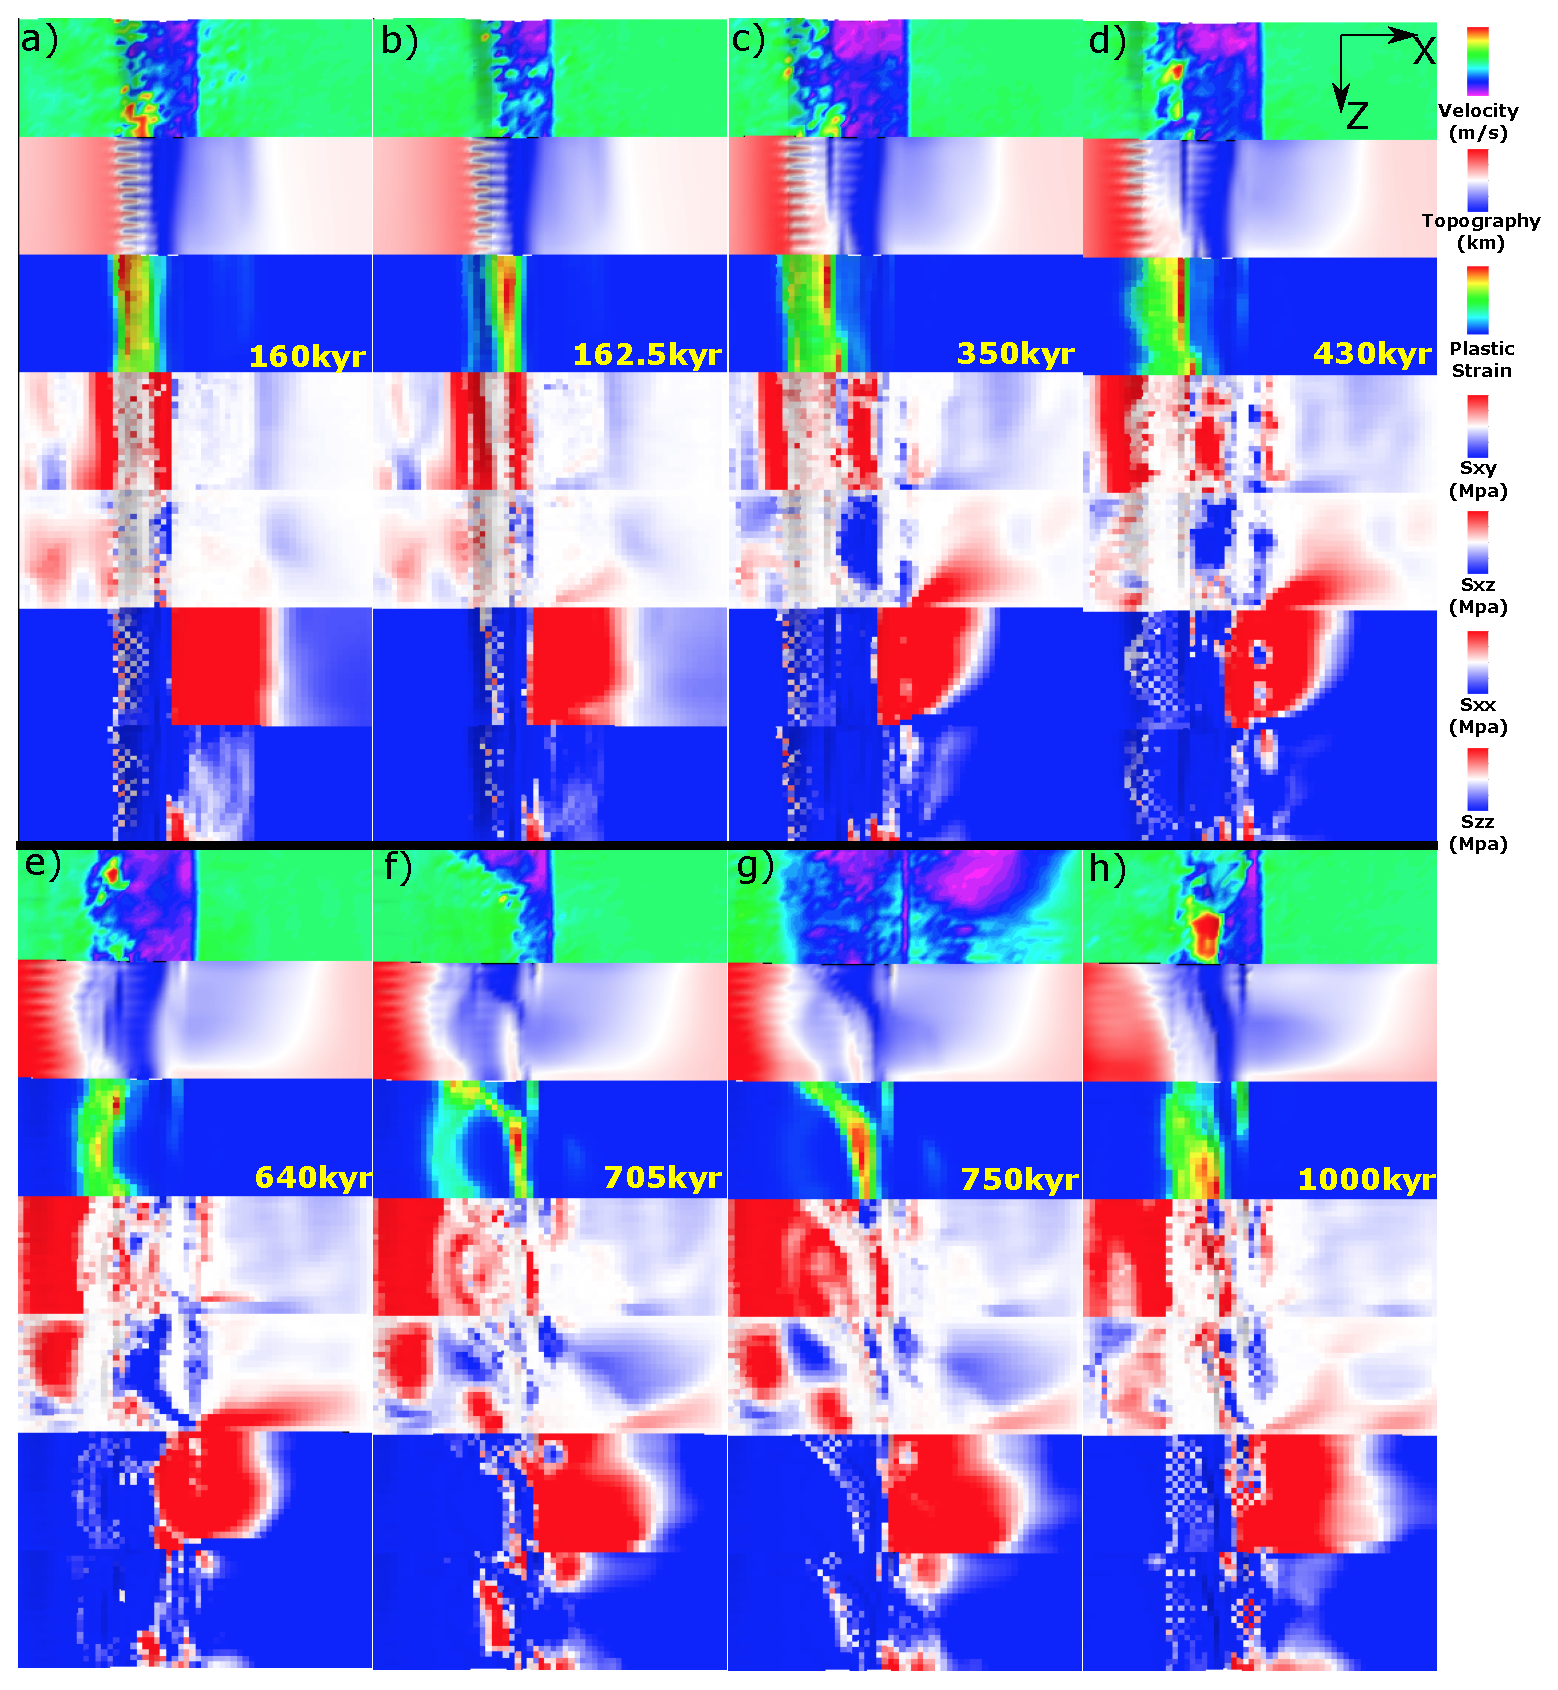
\includegraphics[width=0.8\textwidth]{./Figures/fig_Results_MRange_2_M57LinT1_time_evolution.eps}
 \caption{M57LinT1 (Table~\hyperref[Tab1_1]{\ref{Tab1_1}}) faulting and stresses evolution with respect to time.}
\label{fig_Results_MRange_2}
\end{figure}
       
\iffalse
\subsubsection{M57SqrtT2 versus M58SqrtT2}

For description of evolutio of M58SqrtT2, please refer to Paragraph~\hyperref[para_M58SqrtT2]{\ref{para_M58SqrtT2}}.

The major difference between M57SqrtT2 and M58SqrtT2 is that only M58SqrtT2 has fault alternation.

\paragraph{M57SqrtT2}

\begin{figure}[h]
 \centering
  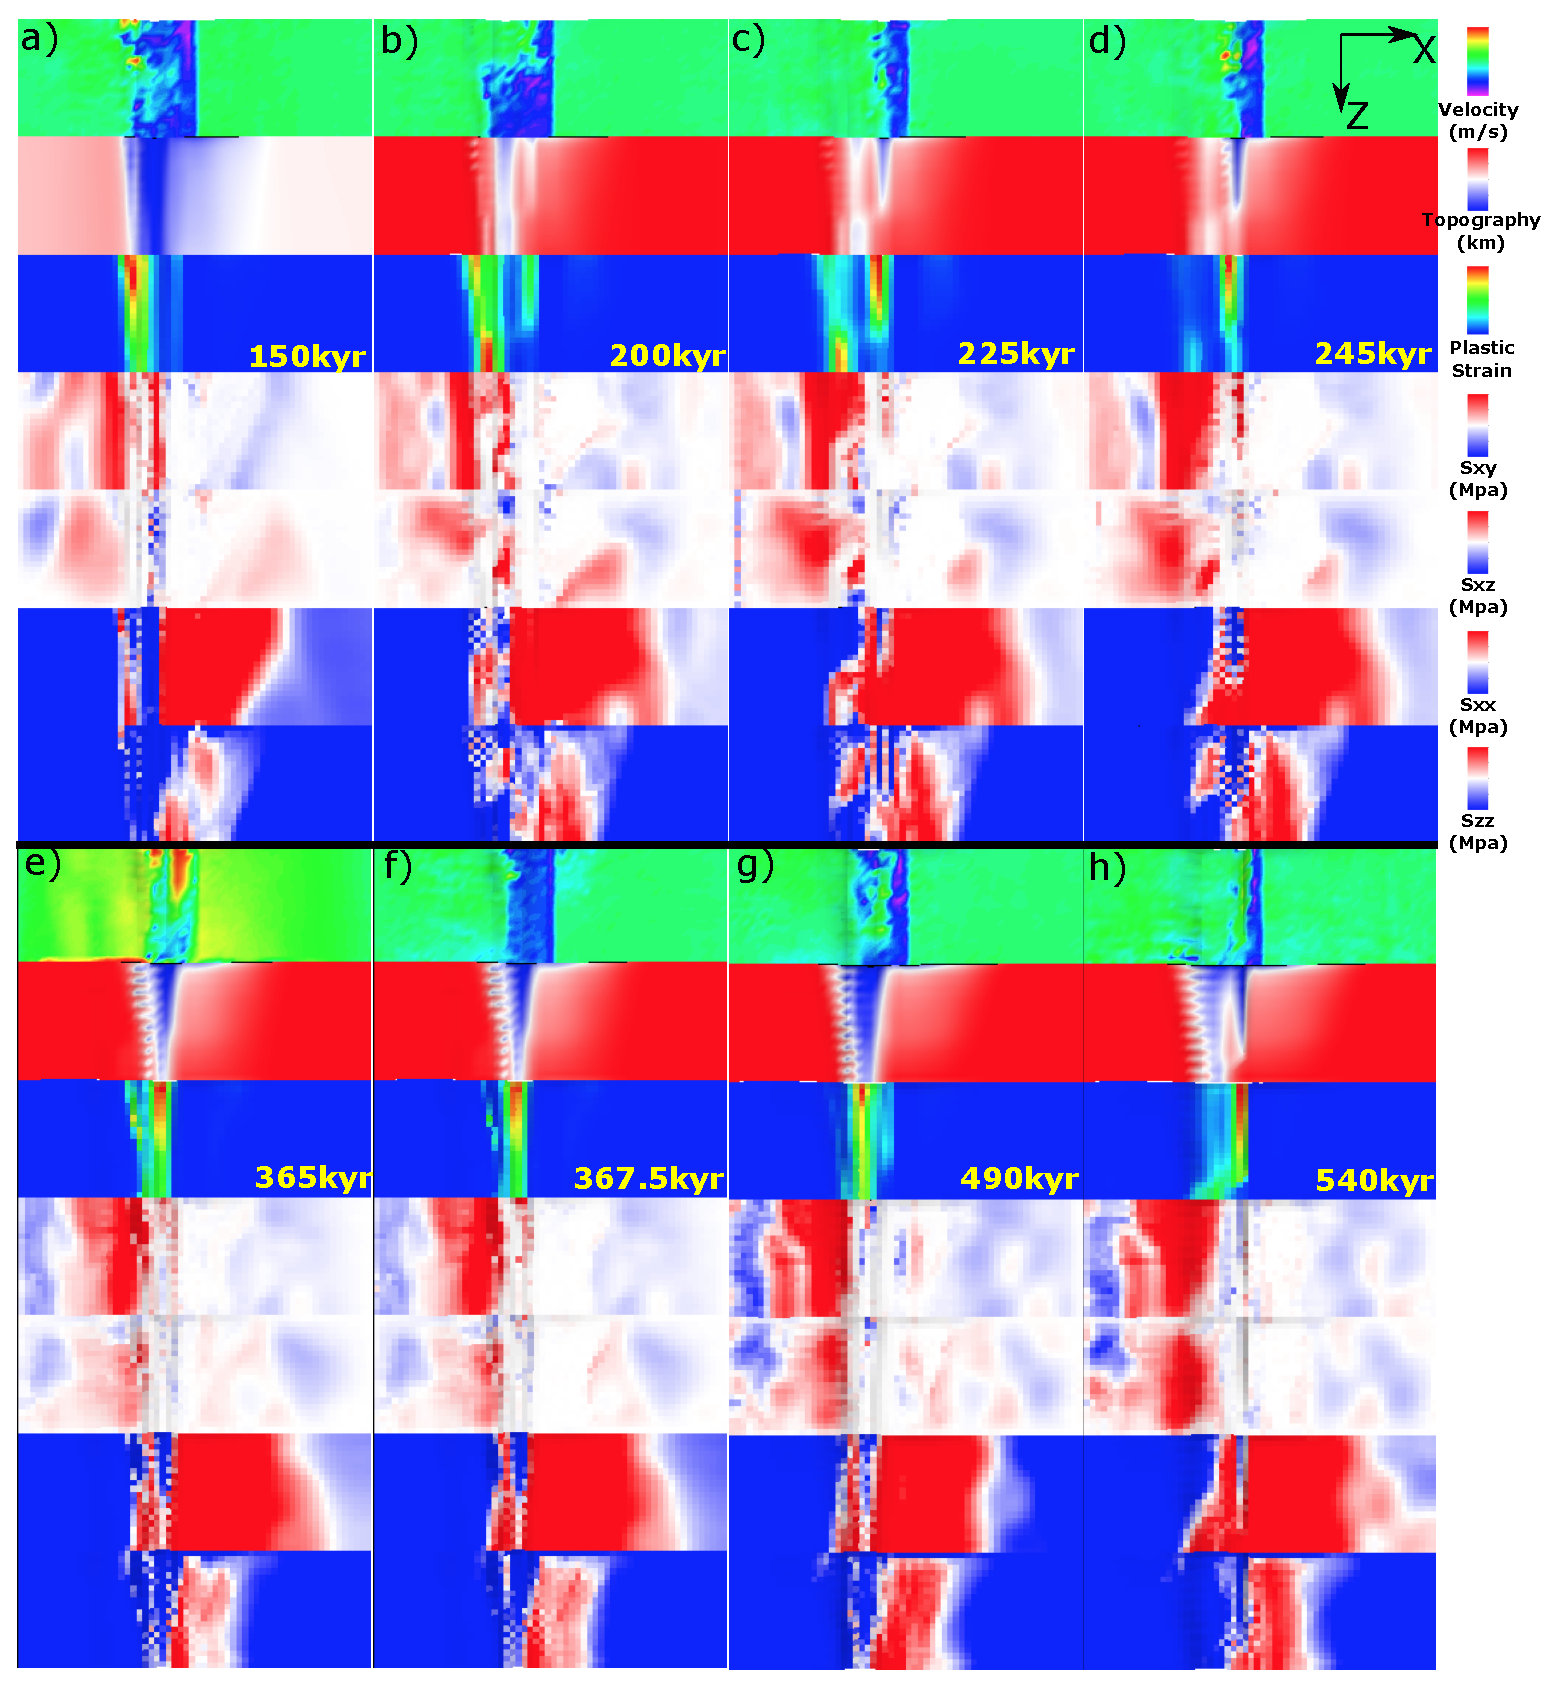
\includegraphics[width=0.8\textwidth]{./Figures/fig_Results_MRange_3_M57SqrtT2_time_evolution.eps}
 \caption{M57SqrtT2 (Table~\hyperref[Tab1_1]{\ref{Tab1_1}}) faulting and stresses evolution with respect to time.}
\label{fig_Results_MRange_3}
\end{figure}

~\\
For M57SqrtT2, six small scale mass wasting happen at 282.5 kyr, 290 kyr, 365 kyr, 452.5 kyr, 482.5 kyr and 540 kyr respectively. As shown in Figure~\hyperref[fig_Results_MRange_3]{\ref{fig_Results_MRange_3}}, the fault keeps on the left-hand side of the ridge axis. By 200 kyr (Figure~\hyperref[fig_Results_MRange_3]{\ref{fig_Results_MRange_3}.b}), an inward fault jump begins to evolve and takes the place of the initial fault. As the fault evolve, a stage of discontinuous abyssal hill is produced at the lower M side (Figure~\hyperref[fig_Results_MRange_3]{\ref{fig_Results_MRange_3}.c}). The fault propagates toward the higher M side and cuts through the plate by $\sim$245 kyr (Figure~\hyperref[fig_Results_MRange_3]{\ref{fig_Results_MRange_3}.d}) when corrugations at the lower M side are produced. Between 365 kyr (Figure~\hyperref[fig_Results_MRange_3]{\ref{fig_Results_MRange_3}.e}) and 367.5 kyr (Figure~\hyperref[fig_Results_MRange_3]{\ref{fig_Results_MRange_3}.f}), a mass wasting happens. By 490 kyr (Figure~\hyperref[fig_Results_MRange_3]{\ref{fig_Results_MRange_3}.g}), an antithetic fault begins to evolve and terminates the old fault. It then develops into a vertical tensile failure at 540 kyr (Figure~\hyperref[fig_Results_MRange_3]{\ref{fig_Results_MRange_3}.h}).
\fi













% Between the \iffalse and \fi are the short version of the three effects of M ranges, functional forms and two type weakening rates. 

\iffalse
\subsection{Effects of the functional forms of M variation}

\subsubsection{Models with M between 0.2 and 0.8 and Type 1 weakening}

Major differences among models with M between 0.2 and 0.8 (M28) and Type 1 (T1) weakening lie in the model behaviors in terms of the inward fault jump, the mass wasting and the hourglass-shaped median valley. None of the three models show fault alternation.    

\begin{figure}[h]
  \centering
    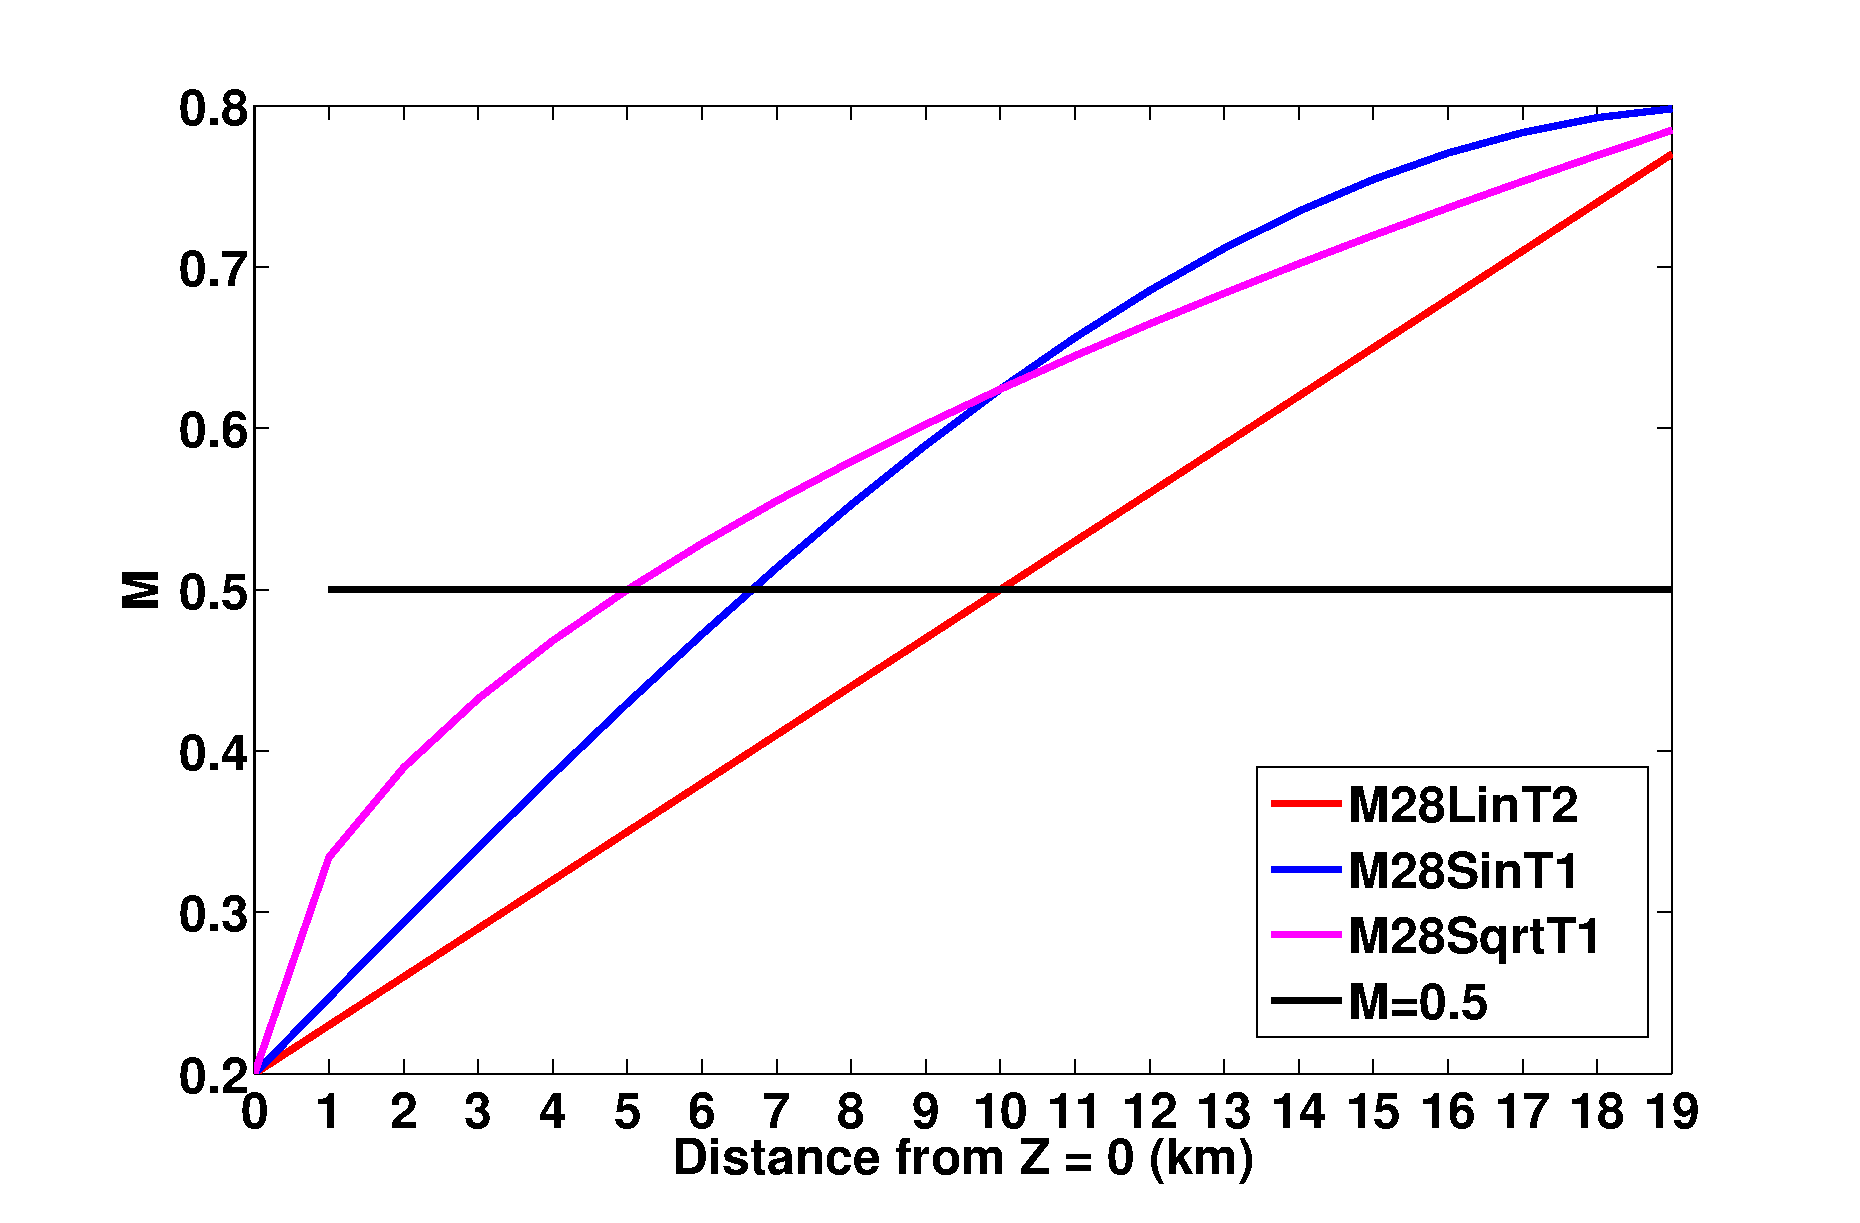
\includegraphics[width=0.8\textwidth]{./Figures/fig_Results_3_3_M_variation.eps}
  \caption{Three functional forms of M variation. M begins to exceed the M $=$ 0.5 black line at Z=10 km, 7 km, 5 km for M28LinT1, M28SinT1 and M28SqrtT1 respectively.}
 \label{fig_Results3_1}
\end{figure}   

\paragraph{Inward fault jump}\label{para_InwardFaultJump}
~\\
Only the models with linear and sinusoidal M variations show inward fault jumps. No inward fault jump occurs when M varies with square root of the along-ridge distance. The termination of a detachment fault retreats towards the ridge axis after a mass wasting and the detachment fault is maintained near the ridge axis.

Timing of inward jumps and the along-strike dimension of the new faults are different between linear and sinusoidal models. The inward jump at the higher M side creates a new fault that accommodates most of the extension at $\sim$900 kyr and replaces the initial detachment fault (Figure~\hyperref[fig_Results4_2]{\ref{fig_Results4_2}}, Figure~\hyperref[fig_Results1_1]{\ref{fig_Results1_1}.f}).
%It nucleates from the ridge center where M $=$ 0.5 and then propagates to the M $=$ 0.8 end with a length of $\sim$11 km. 
 %This secondary fault creates another dome with initial composition likely to be volcanic rather than ultramafic, however, as it evolves, if it can last long enough to cut through the whole crust, mantle materials might exhume to the surface. The composition of the domes observed at Kane magamullions is similar to this mechanism between ultramafic babel dome and eastern to it the crustal inside-corner high.  its spatial distribution is at M$>0.5$ region.
The first inward fault jump occurs earlier in a sinusoidal model (e.g., at $\sim$550 kyr in MXXSinXX)than in the linear reference model. Also, the along-strike length of the new fault in the sinusoidal model is $\sim$14 km (Figure~\hyperref[fig_Results4_2]{\ref{fig_Results4_2}}).
%
The timing difference between the linear and sinusoidal models is because M28SinT1 consistently has a higher M values than the M28LinT1 (Figure~\hyperref[fig_Results3_1]{\ref{fig_Results3_1}}), which results in that the initial detachment fault at the higher M side (M $>$ 0.5) of M28SinT1 is pushed off axis faster than M28LinT1 and thus forming an earlier inward fault jump. The length difference is because M28SinT1 has a greater length along the ridge axis of M $\ge$ 0.5 (Figure~\hyperref[fig_Results3_1]{\ref{fig_Results3_1}}). 
%
\begin{figure}[h]
  \centering
    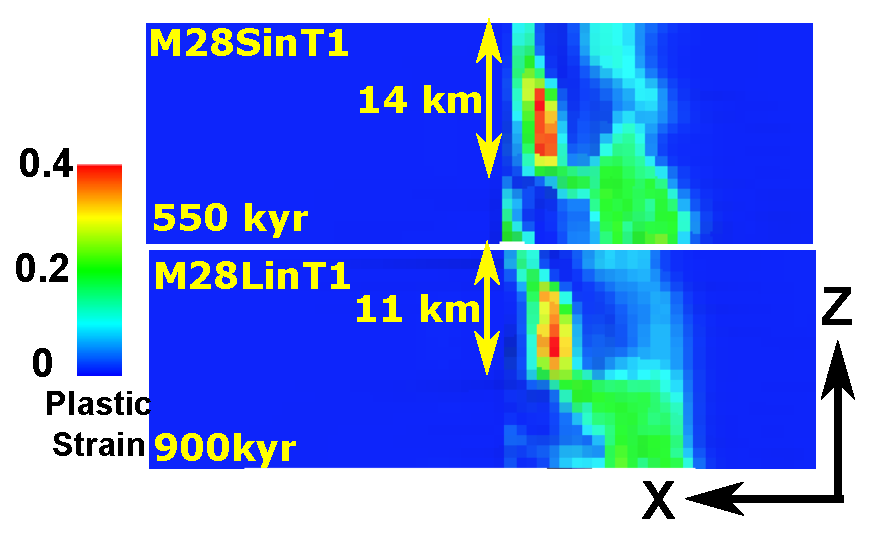
\includegraphics[width=0.6\textwidth]{./Figures/fig_Results4_2_secondary_fault_length_comparison1.eps}
  \caption{Bird's-eye view for comparing the length and timing of inward fault jump.}
 \label{fig_Results4_2}
\end{figure}

\paragraph{Mass wasting}

\begin{figure}[h]
  \centering
    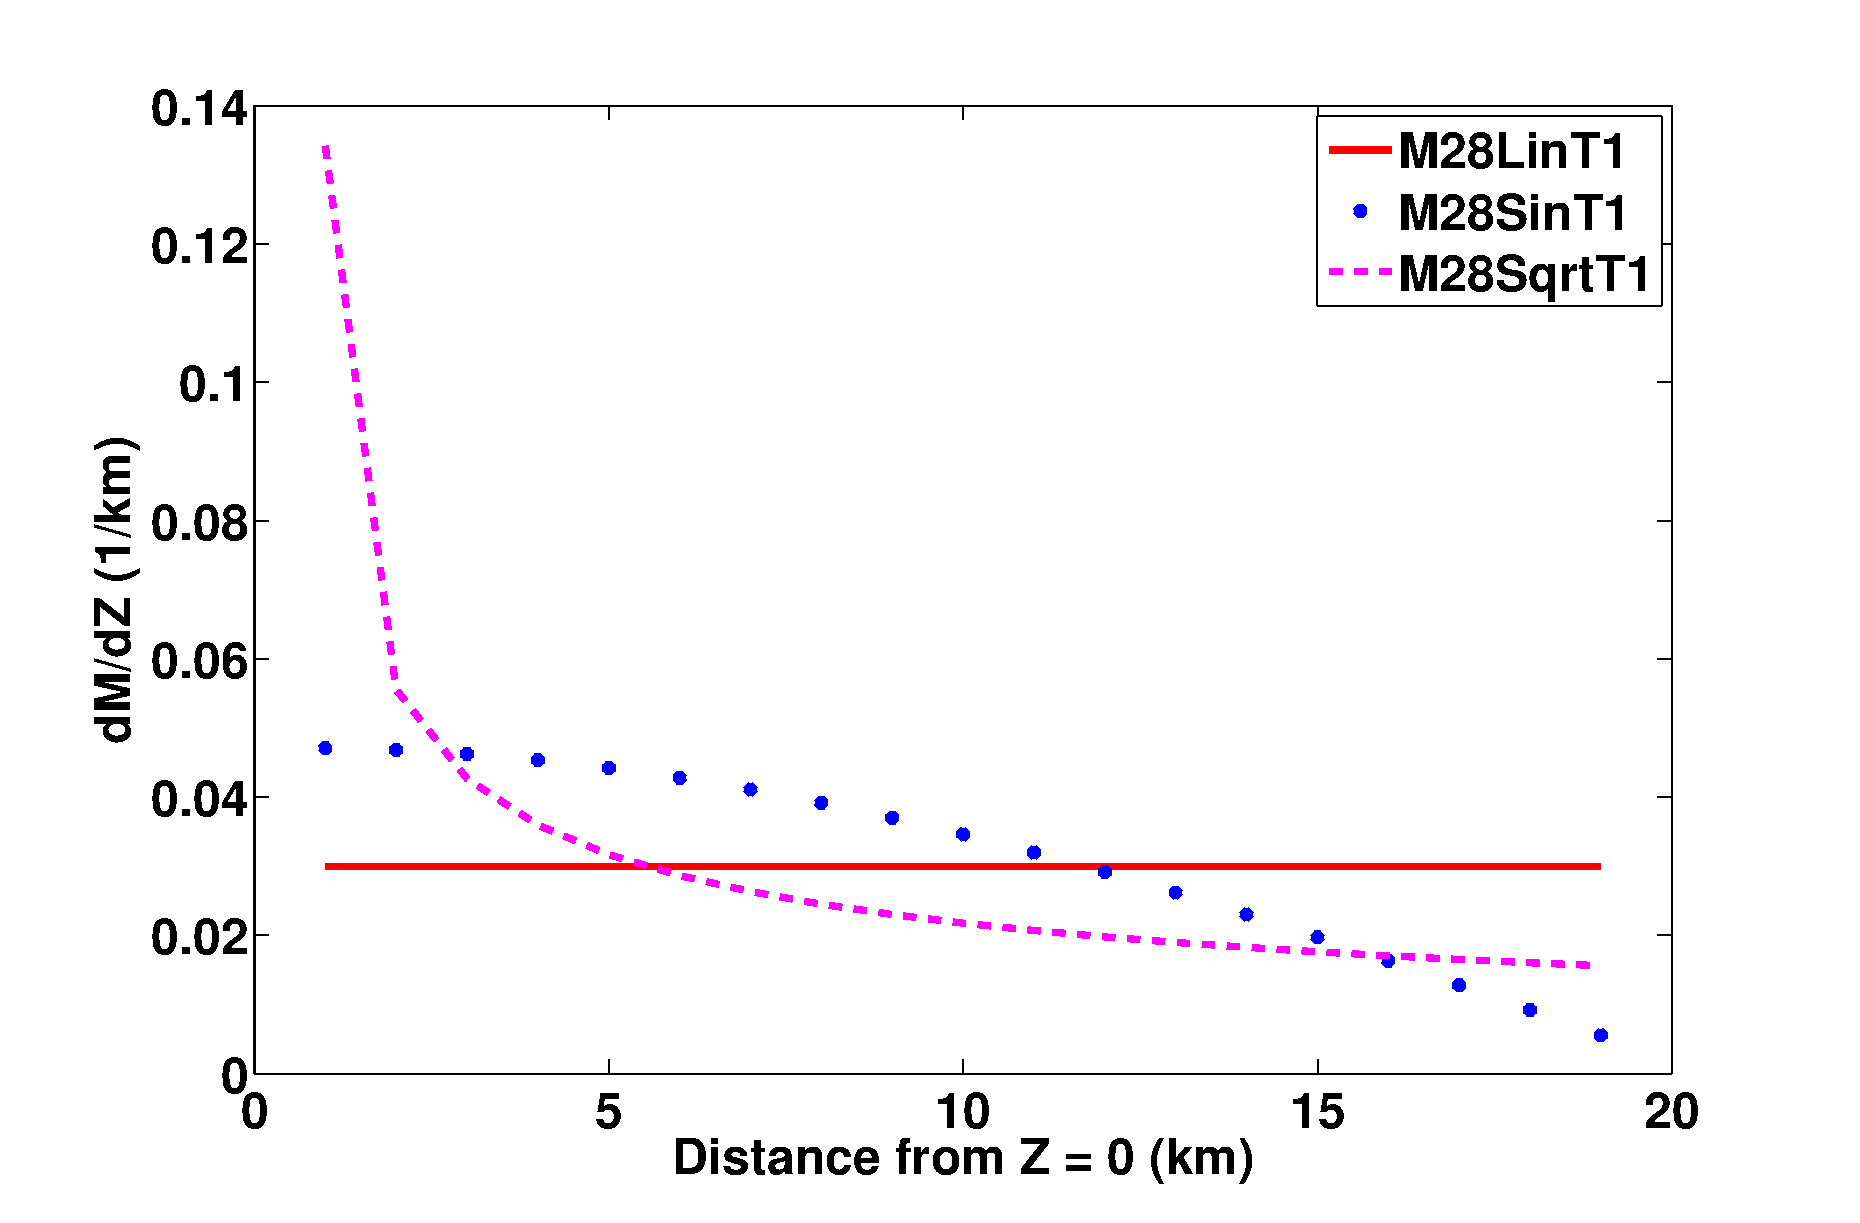
\includegraphics[width=0.8\textwidth]{./Figures/fig_Results_3_3_1_M_type_plot_dM_dZ.eps}
  \caption{$\partial M/ \partial Z$ comparision.}
 \label{fig_Results_3_3_1_M_type_plot_dM_dZ}
\end{figure}  

~\\
Mass wasting occurs only in the square root model among thoe group of M28 and T1. Qualitatively, it is because the square root profile of M variation has a much higher value of $\frac{\partial M}{\partial Z}$ at the lower M side (Figure~\hyperref[fig_Results_3_3_1_M_type_plot_dM_dZ]{\ref{fig_Results_3_3_1_M_type_plot_dM_dZ}}), which implies a larger along-ridge shear stress $\sigma_{xz}$ as well as a larger difference in $\sigma_{xy}$ along the ridge that result in the decoupling between the higher and lower M sides hanging walls.\note[EC]{can't understand the last sentence.}

\iffalse
\begin{figure}[h]
  \centering
    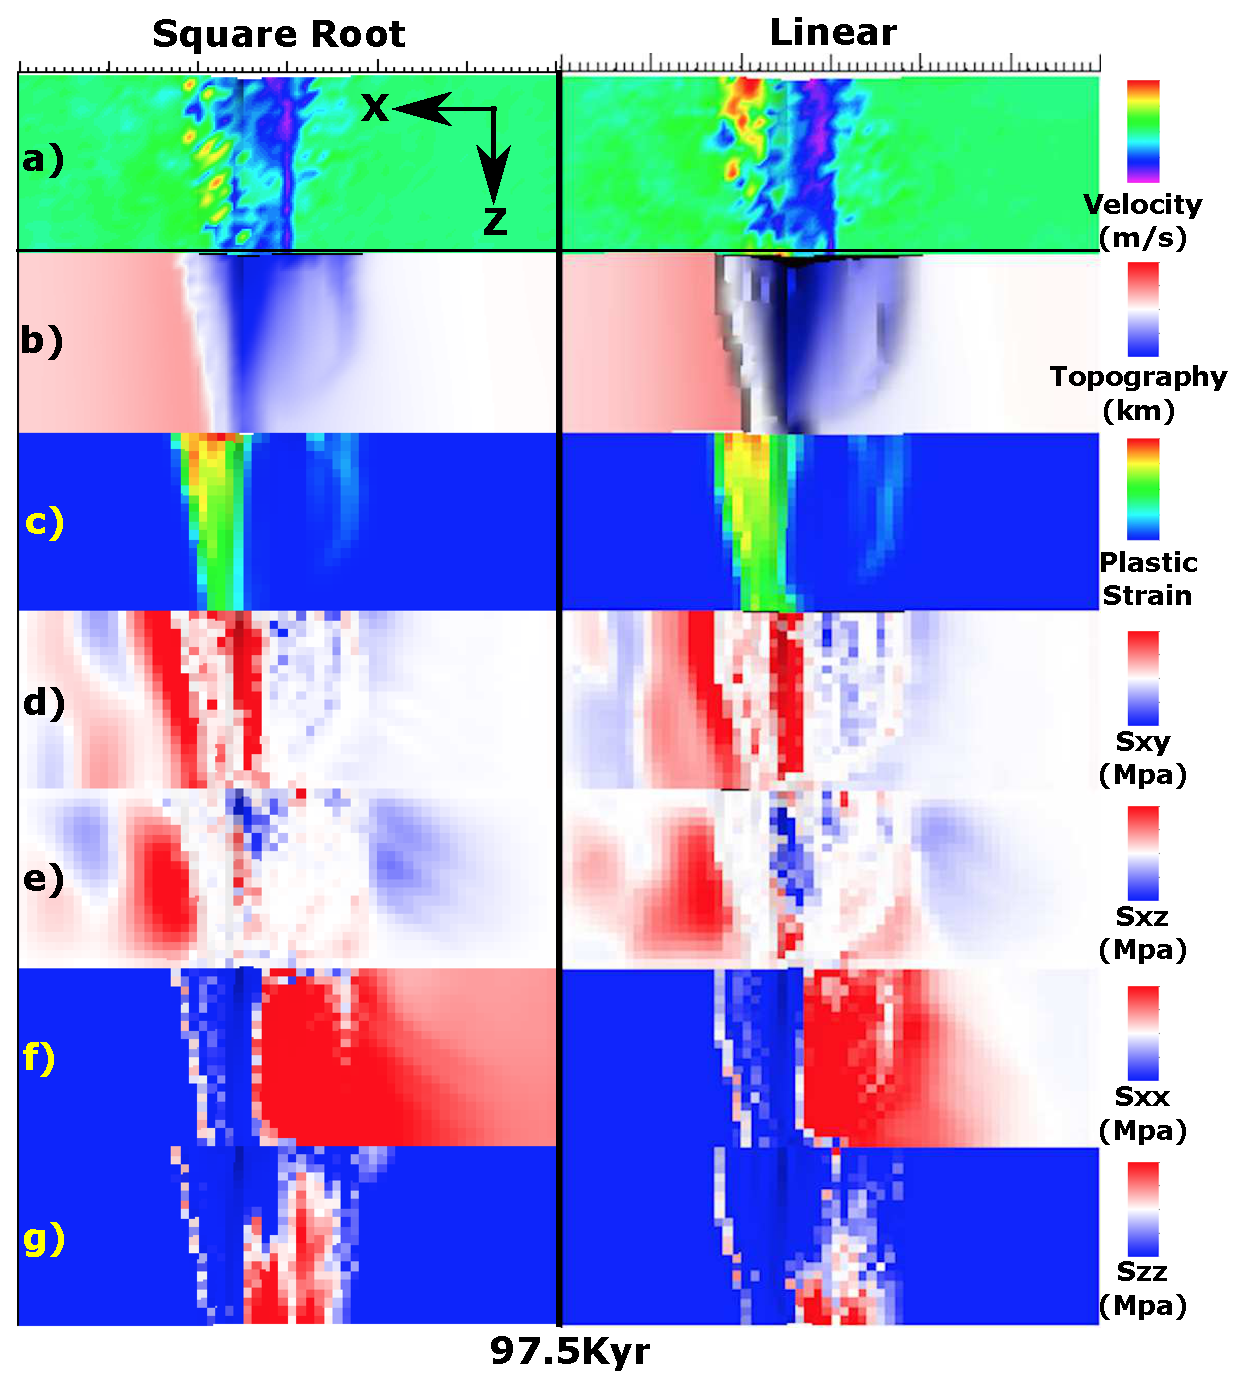
\includegraphics[width=0.6\textwidth]{./Figures/fig_Results4_3_sqrt_vs_lin_cut_back_97kyr.eps}
  \caption{M28LinT1 versus M28SqrtT1 (Table~\hyperref[Tab1_1]{\ref{Tab1_1}}) at 97 kyr. View from top of the model.}
 \label{fig_Results4_3_1}
\end{figure}  

\begin{figure}[h]
  \centering
    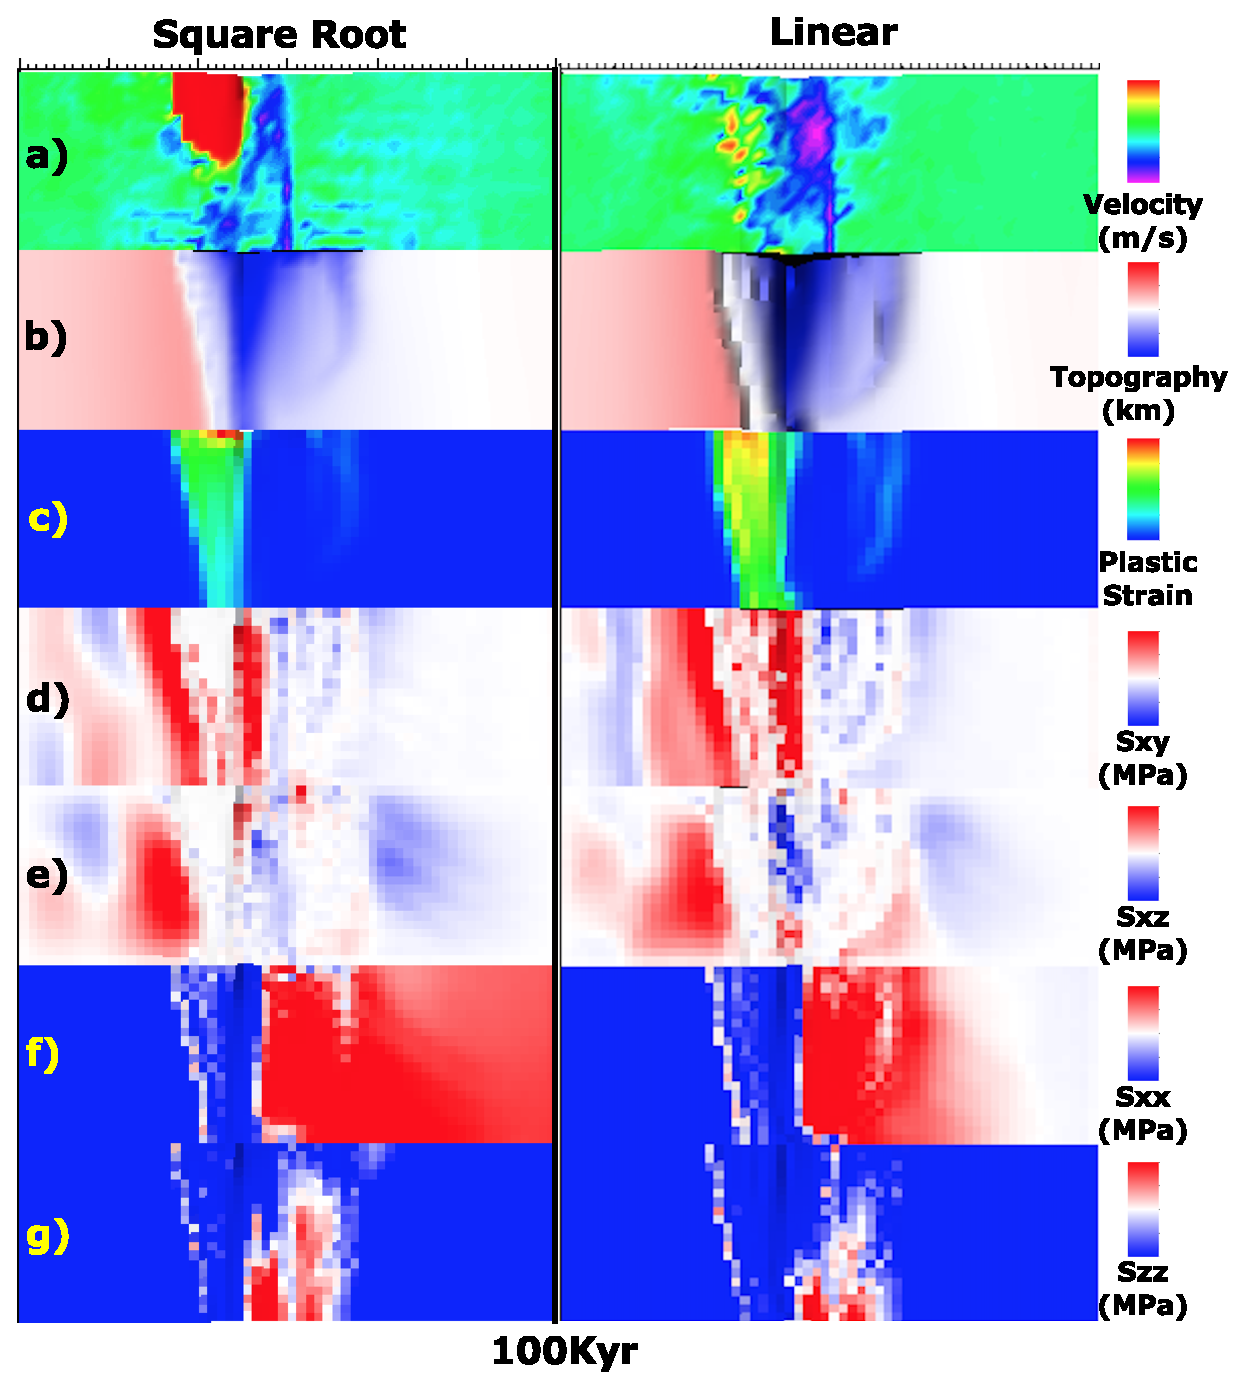
\includegraphics[width=0.6\textwidth]{./Figures/fig_Results4_3_sqrt_vs_lin_cut_back_100kyr.eps}
  \caption{M28LinT1 versus M28SqrtT1 (Table~\hyperref[Tab1_1]{\ref{Tab1_1}}) at 100 kyr. View from top of the model.}
 \label{fig_Results4_3_2}
\end{figure} 
\fi

\paragraph{Hourglass-shaped median valley}
~\\
As shown in Figure~\hyperref[fig_Results_3_3_1_hourglass]{\ref{fig_Results_3_3_1_hourglass}}, differences among the three models are identified. At 160 kyr, the median valley in the model M28SinT1 has \annote[EC]{the smallest cross sectional ($x$-$y$) area}{You can't call it a cross-sectional area. Maybe a map-view area? Or just width? And I don't see if it's really the smallest in M28SinT1.} at the higher M side. \annote[EC]{While}{You can't use while this way. Please look up the usage of this word.} At the lower M side, the square root model has the smallest area of the cross-section. This is because the \change[EC]{cross-section area inside}{width of} the median valley is inversely proportional to the local M value along the ridge. Moreover, the \annote[EC]{breakaways}{Mark these on the figure.} at the lowest M value in the linear and sinusoidal models becomes parallel to the ridge axis while the breakaway of the square root model maintains the oblique trend. \annote[EC]{In addition, M28SinT1 has a trough inside the median valley with the highest curvature.}{I can't see this. Can you mark this on the figure?} At 500 kyr, M28SinT1 has \annote[EC]{the narrowest median valley}{Still can't agree.} at the higher M side and the high topography zone on the left-hand side of the ridge axis is the widest. Integrating the topography at the left-hand side of the ridge axis of the three models, M28Sqrt has the largest value of integration since it has the largest integration of M along the ridge axis \note[EC]{Did you actually do the integration? Integrating over what? Why integration? Why the largest integration of M means the greatest integration of topography?}.
% In addition, the termination of the detachment fault of M28SqrtT1 has the highest curvature at the lower M sides. All these observations correspond to the M variation (Figure~\hyperref[fig_Results3_1]{\ref{fig_Results3_1}}).
\begin{figure}[h]
  \centering
    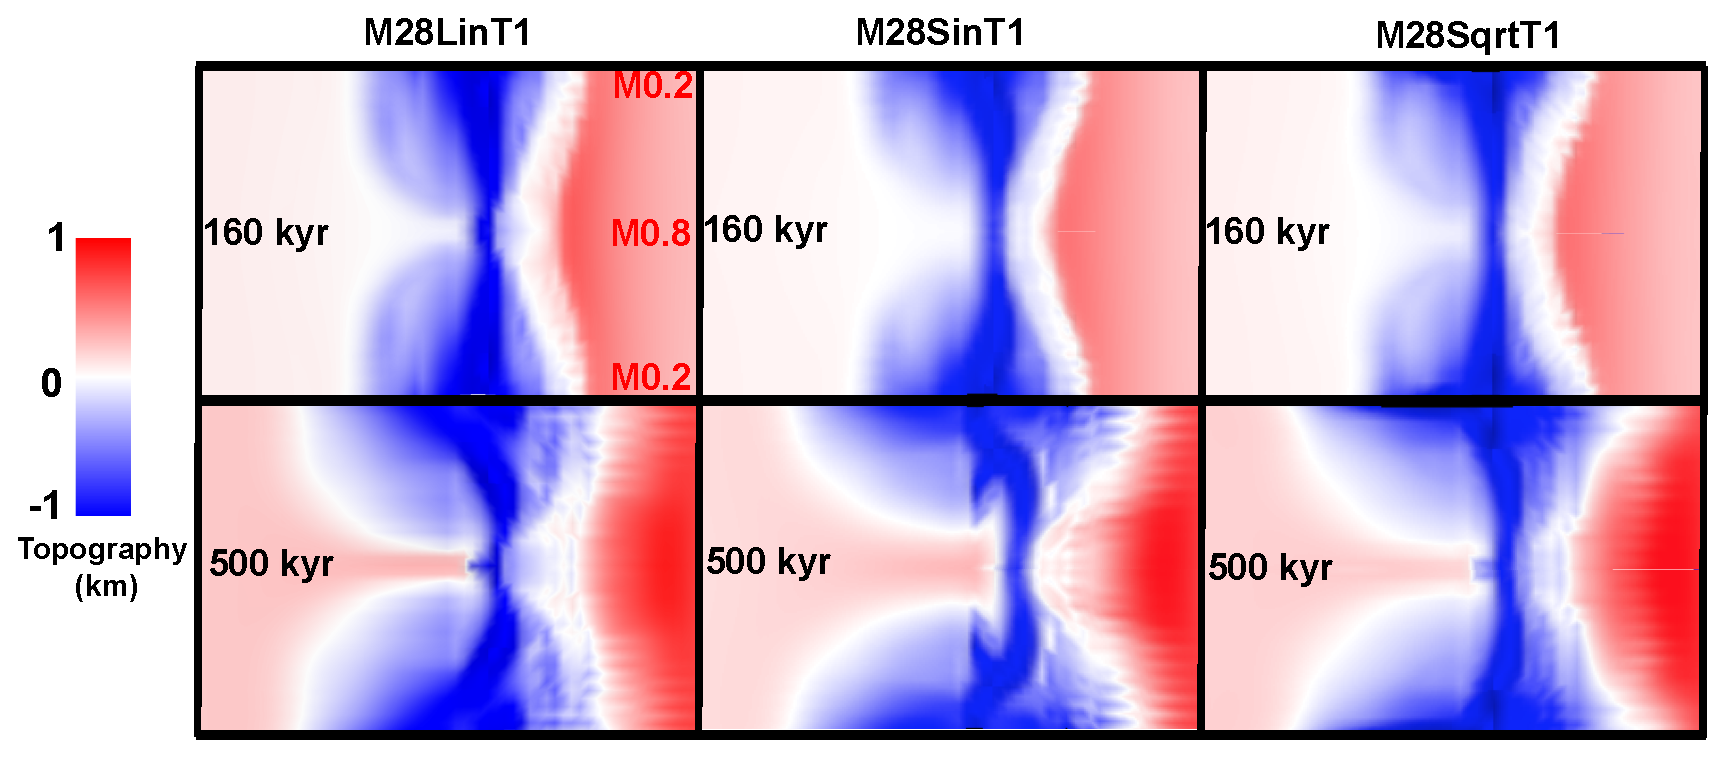
\includegraphics[width=1.0\textwidth]{./Figures/fig_Results_3_3_1_hourglass.eps}
  \caption{Bird's-eye view of the topograpy. \annote[EC]{(without vertical exaggeration.)}{don't need to say. When you did it, you need to say so.} \note[EC]{Say somewhere that you put the origianl and an mirror iamage together in this figure.}}
 \label{fig_Results_3_3_1_hourglass}
\end{figure} 

\subsection{Effects of the weakening rate}

Among the eleven 3D models, three pairs of models have the same parameters but differ only in the weakening rate: M57SinT1/T2, M58SinT1/T2 and M58SqrtT1/T2. I compare them pairwise to single out the effects of the weakening rate on the model behaviors.

%\subsubsection{M57SinT1 versus M57SinT2}

\begin{figure}[h]
 \centering
  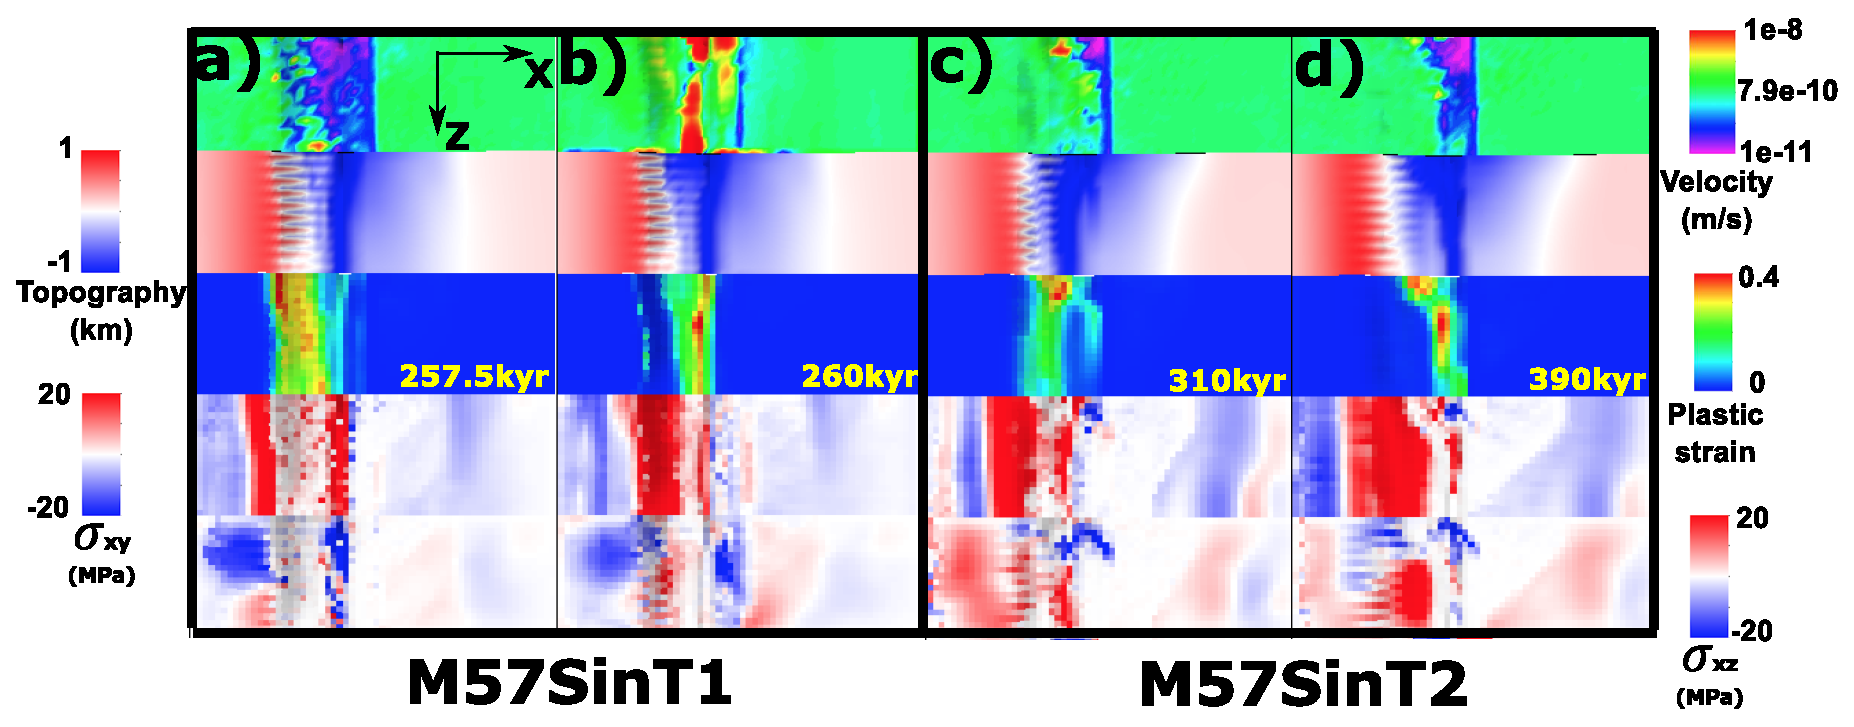
\includegraphics[width=1.0\textwidth]{./Figures/fig_Results_Weakening_2_M57SinT1VST2_CutbackVSsecondaryFault.eps}
 \caption{M57SinT2 versus M57SinT1 (Table~\hyperref[Tab1_1]{\ref{Tab1_1}})}
\label{fig_Results_Weakenging_2}
\end{figure}
~\\
Initially, both M57SinT1 and M57SinT2 develop normal faults on both sides of the ridge axis at the lower M side. However, the faults complete propagation towards the higher M side earlier in the fast-weakening model (M57SinT1) than in the slow-weakening model (M57SinT2). In M57SinT1, a mass wasting event occurs at $\sim$260 kyr but %and helps to maintain a relative higher angle fault with a termination closer to the ridge axis. 
the initial fault remains active without experiencing an inward fault jump (Figure~\hyperref[fig_Results_Weakenging_2]{\ref{fig_Results_Weakenging_2}.a and b}). In contrast, the slower-weakening model experiences an inward fault jump at the higher M side (M $>$ \annote[EC]{0.55}{Since the range is 0.5-0.7, isn't this value on the lower M side?}) but the initial fault remains active in the M $<$ 0.55 region (Figure~\hyperref[fig_Results_Weakenging_2]{\ref{fig_Results_Weakenging_2}.c and d}).\note[EC]{Without further annotations on the figure, referring to the figure wouldn't help much.}
The width of the `'median valley at the lower M side is wider in M57SinT2 than in M57SinT1 (Figure~\hyperref[fig_Results_Weakenging_2]{\ref{fig_Results_Weakenging_2}.c, d versus a, b})\note[EC]{Again, the figure doesn't help much because one wouldn't know where to look to visually measure the width.}% because the slower weakening (T2) allows a more distributed tensional stress $\sigma_{xx}$ rather than fast weakening that once a fault establishes, larger amount of the tensional stress $\sigma_{xx}$ is released at the fault. 
The amplitude of the corrugations of the faster-weakening model (M57SinT1) is greater because the faster weakening rate allows a faster decrease in the cohesion and the lowered cohesion promotes tensile failure in the isochron-parallel direction, which produces the corrugations.

\begin{figure}[h]
 \centering
  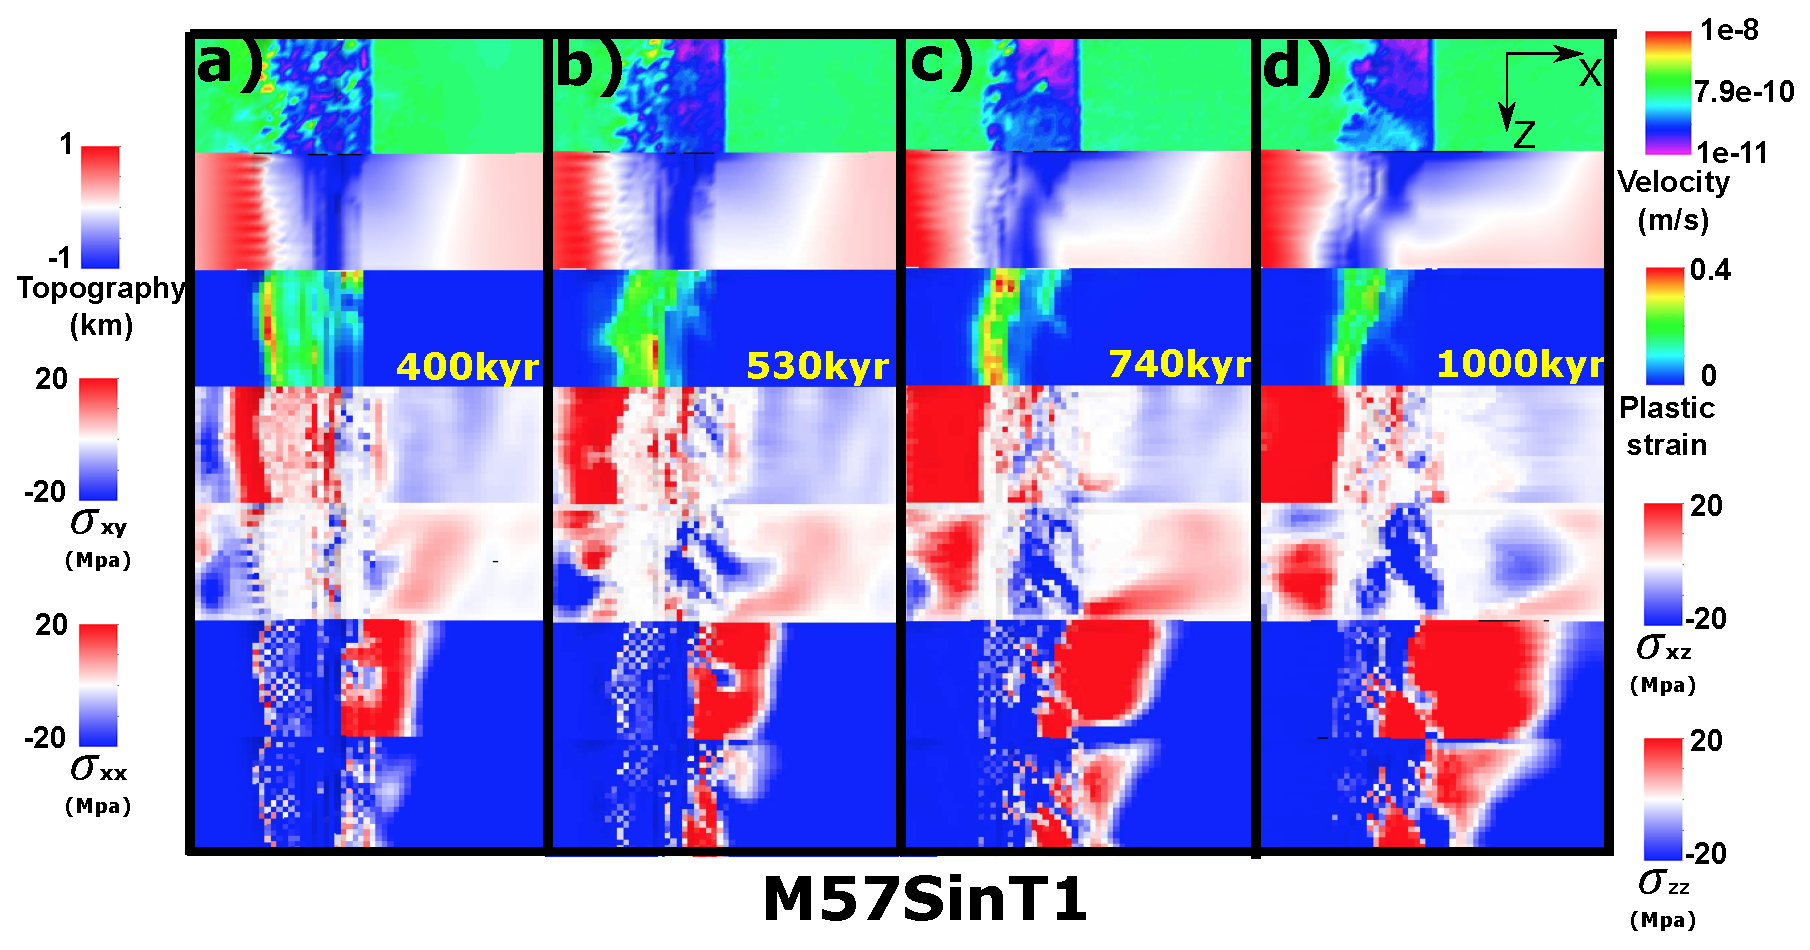
\includegraphics[width=1.0\textwidth]{./Figures/fig_Results_Weakening_3_M57SinT1_time_evolution.eps}
 \caption{Faulting and stresses evolution for M57SinT1.}
\label{fig_Results_Weakenging_3}
\end{figure}

% \paragraph{M57SinT1}\label{para_M57SinT1}
% ~\\
% For M57SinT1, by 400 kyr (Figure~\hyperref[fig_Results_Weakenging_3]{\ref{fig_Results_Weakenging_3}.a}), two antithetic fault forms at the lower M side (0.5 $<$ M $<$ 0.58) accommodating part of the plates extension. This makes the termination at the lower M side retreat backward to the ridge axis. The hanging walls of the antithetic faults slide down into the trough and lower the topography. By 530 kyr, the termination at the center of the ridge segment (M $=$ 0.61$\sim$0.63) extends further (Figure~\hyperref[fig_Results_Weakenging_3]{\ref{fig_Results_Weakenging_3}.b}). This curved termination leads to a curved topography aligns with it (white curve in the second row). By 740 kyr, another antithetic fault forms at the lower M side (Figure~\hyperref[fig_Results_Weakenging_3]{\ref{fig_Results_Weakenging_3}.c}). It doesn't take the place of initial fault and disapear soon, however, it again releases tensional stress and helps maintain a closer to ridge axis termination at the lower M side. By 1000 kyr (Figure~\hyperref[fig_Results_Weakenging_3]{\ref{fig_Results_Weakenging_3}.d}), an Atlantiss Massif shape OCC is produced (lower M side has a wider dome and higher M side has a narrower dome) due to the along ridge termination evolution. Corrugations with wavelength varying from hundreds to kilometers are also produced.       

% \begin{figure}[h]
%  \centering
%   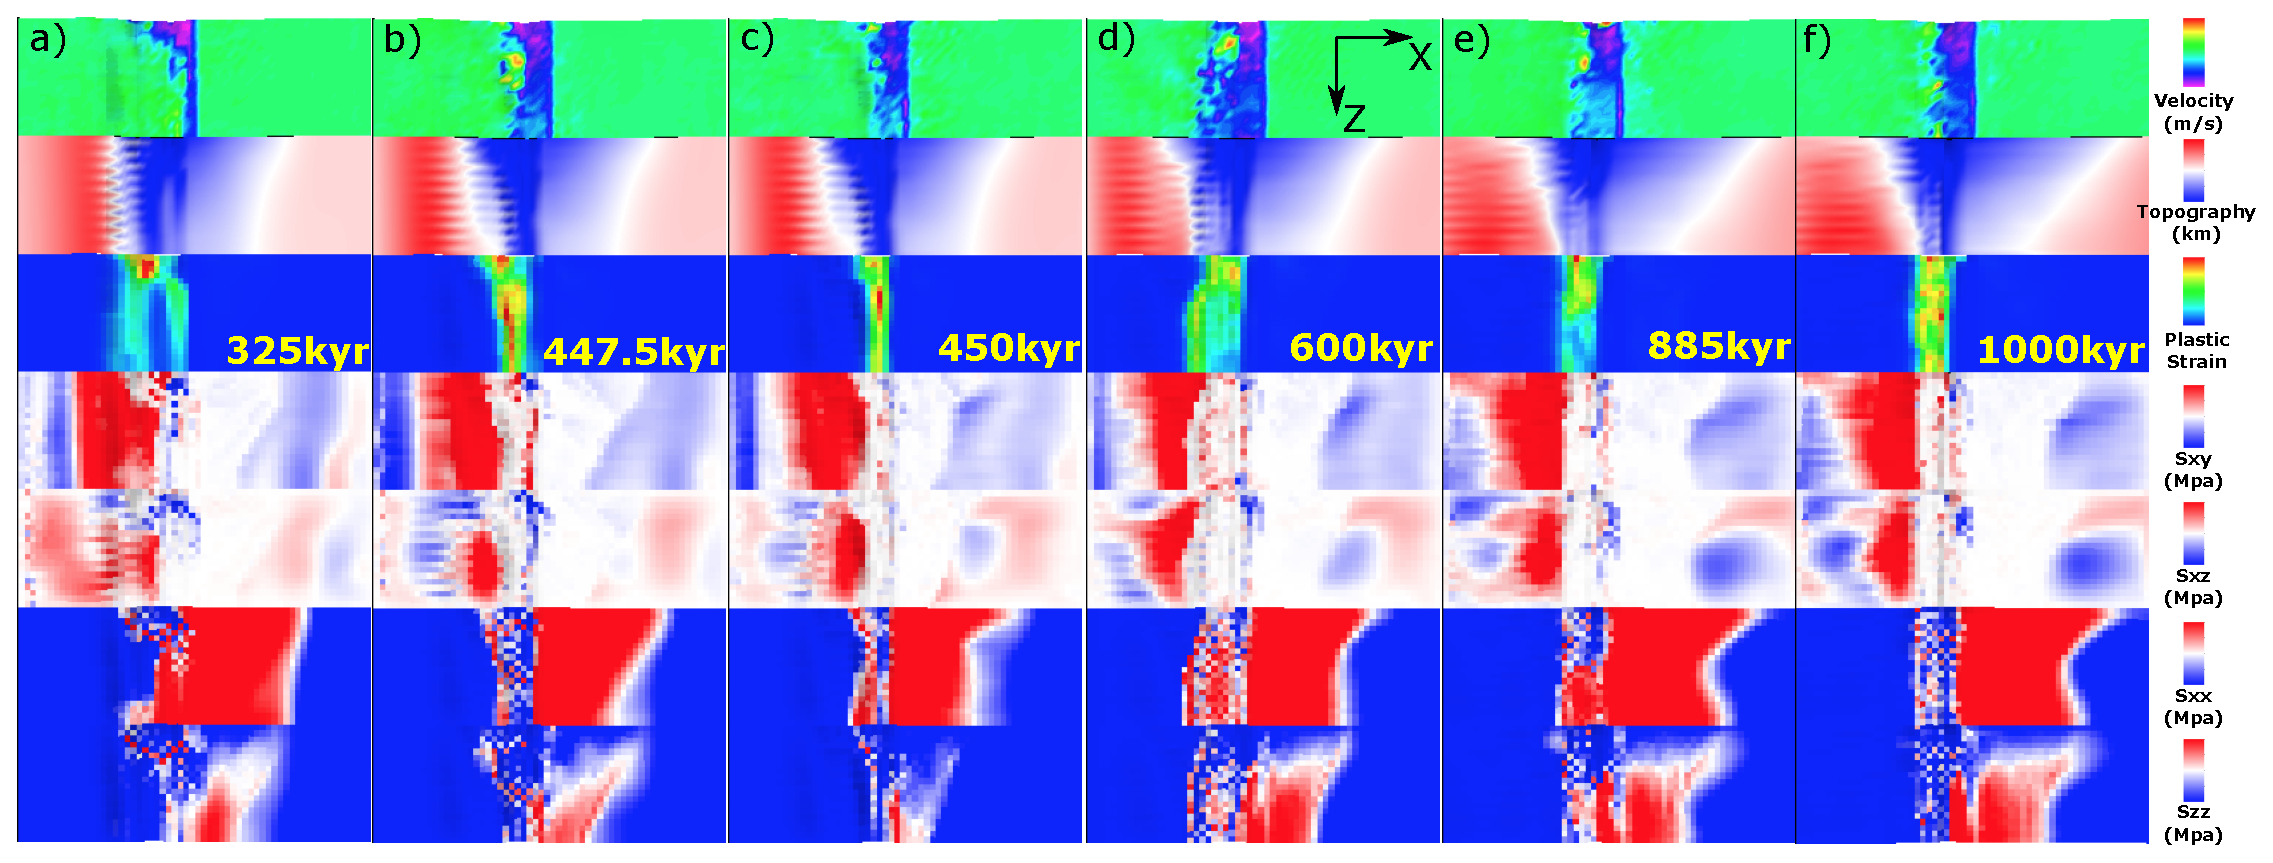
\includegraphics[width=1.0\textwidth]{./Figures/fig_Results_Weakening_4_M57SinT2_time_evolution.eps}
%  \caption{M57SinT2 (Table~\hyperref[Tab1_1]{\ref{Tab1_1}}) faulting and stress evolution with respect to time.}
% \label{fig_Results_Weakenging_4}
% \end{figure}

% \paragraph{M57SinT2}\label{para_M57SinT2}
% ~\\
% For M57SinT2, instead of maintaining a detachment fault like M57SinT1, it produces inward fault jump at the higher M side. By 325 kyr (Figure~\hyperref[fig_Results_Weakenging_4]{\ref{fig_Results_Weakenging_4}.a}), an inward fault jump happens and takes the place of the initial detachment fault at the higher M side. Between 447.5 kyr (Figure~\hyperref[fig_Results_Weakenging_4]{\ref{fig_Results_Weakenging_4}.b}) and 450 kyr (Figure~\hyperref[fig_Results_Weakenging_4]{\ref{fig_Results_Weakenging_4}.c}), a small scale cut-back happens and the termination recedes backward. By 600 kyr, the termination at the higher M side extends further (Figure~\hyperref[fig_Results_Weakenging_4]{\ref{fig_Results_Weakenging_4}.d}). By 885 kyr, an inward fault jump happens at the higher M side (0.62 $<$ M $<$ 0.7) (Figure~\hyperref[fig_Results_Weakenging_4]{\ref{fig_Results_Weakenging_4}.e}). The width of the median valley at the lower M side keeps increasing due to the distributed $\sigma_{xx}$ (Figure~\hyperref[fig_Results_Weakenging_4]{\ref{fig_Results_Weakenging_4}.a$\sim$d}).

The pairs, M58SinT1/T2 and M58SqrtT1/T2, show a consistent difference that the fault alternation occurs only in the slow weakening models.

% \subsubsection{M58SinT1 versus M58SinT2}

% A major difference between M58SinT1 and M58SinT2 is that only M58SinT2 has fault alternation.

% \begin{figure}[h]
%  \centering
%   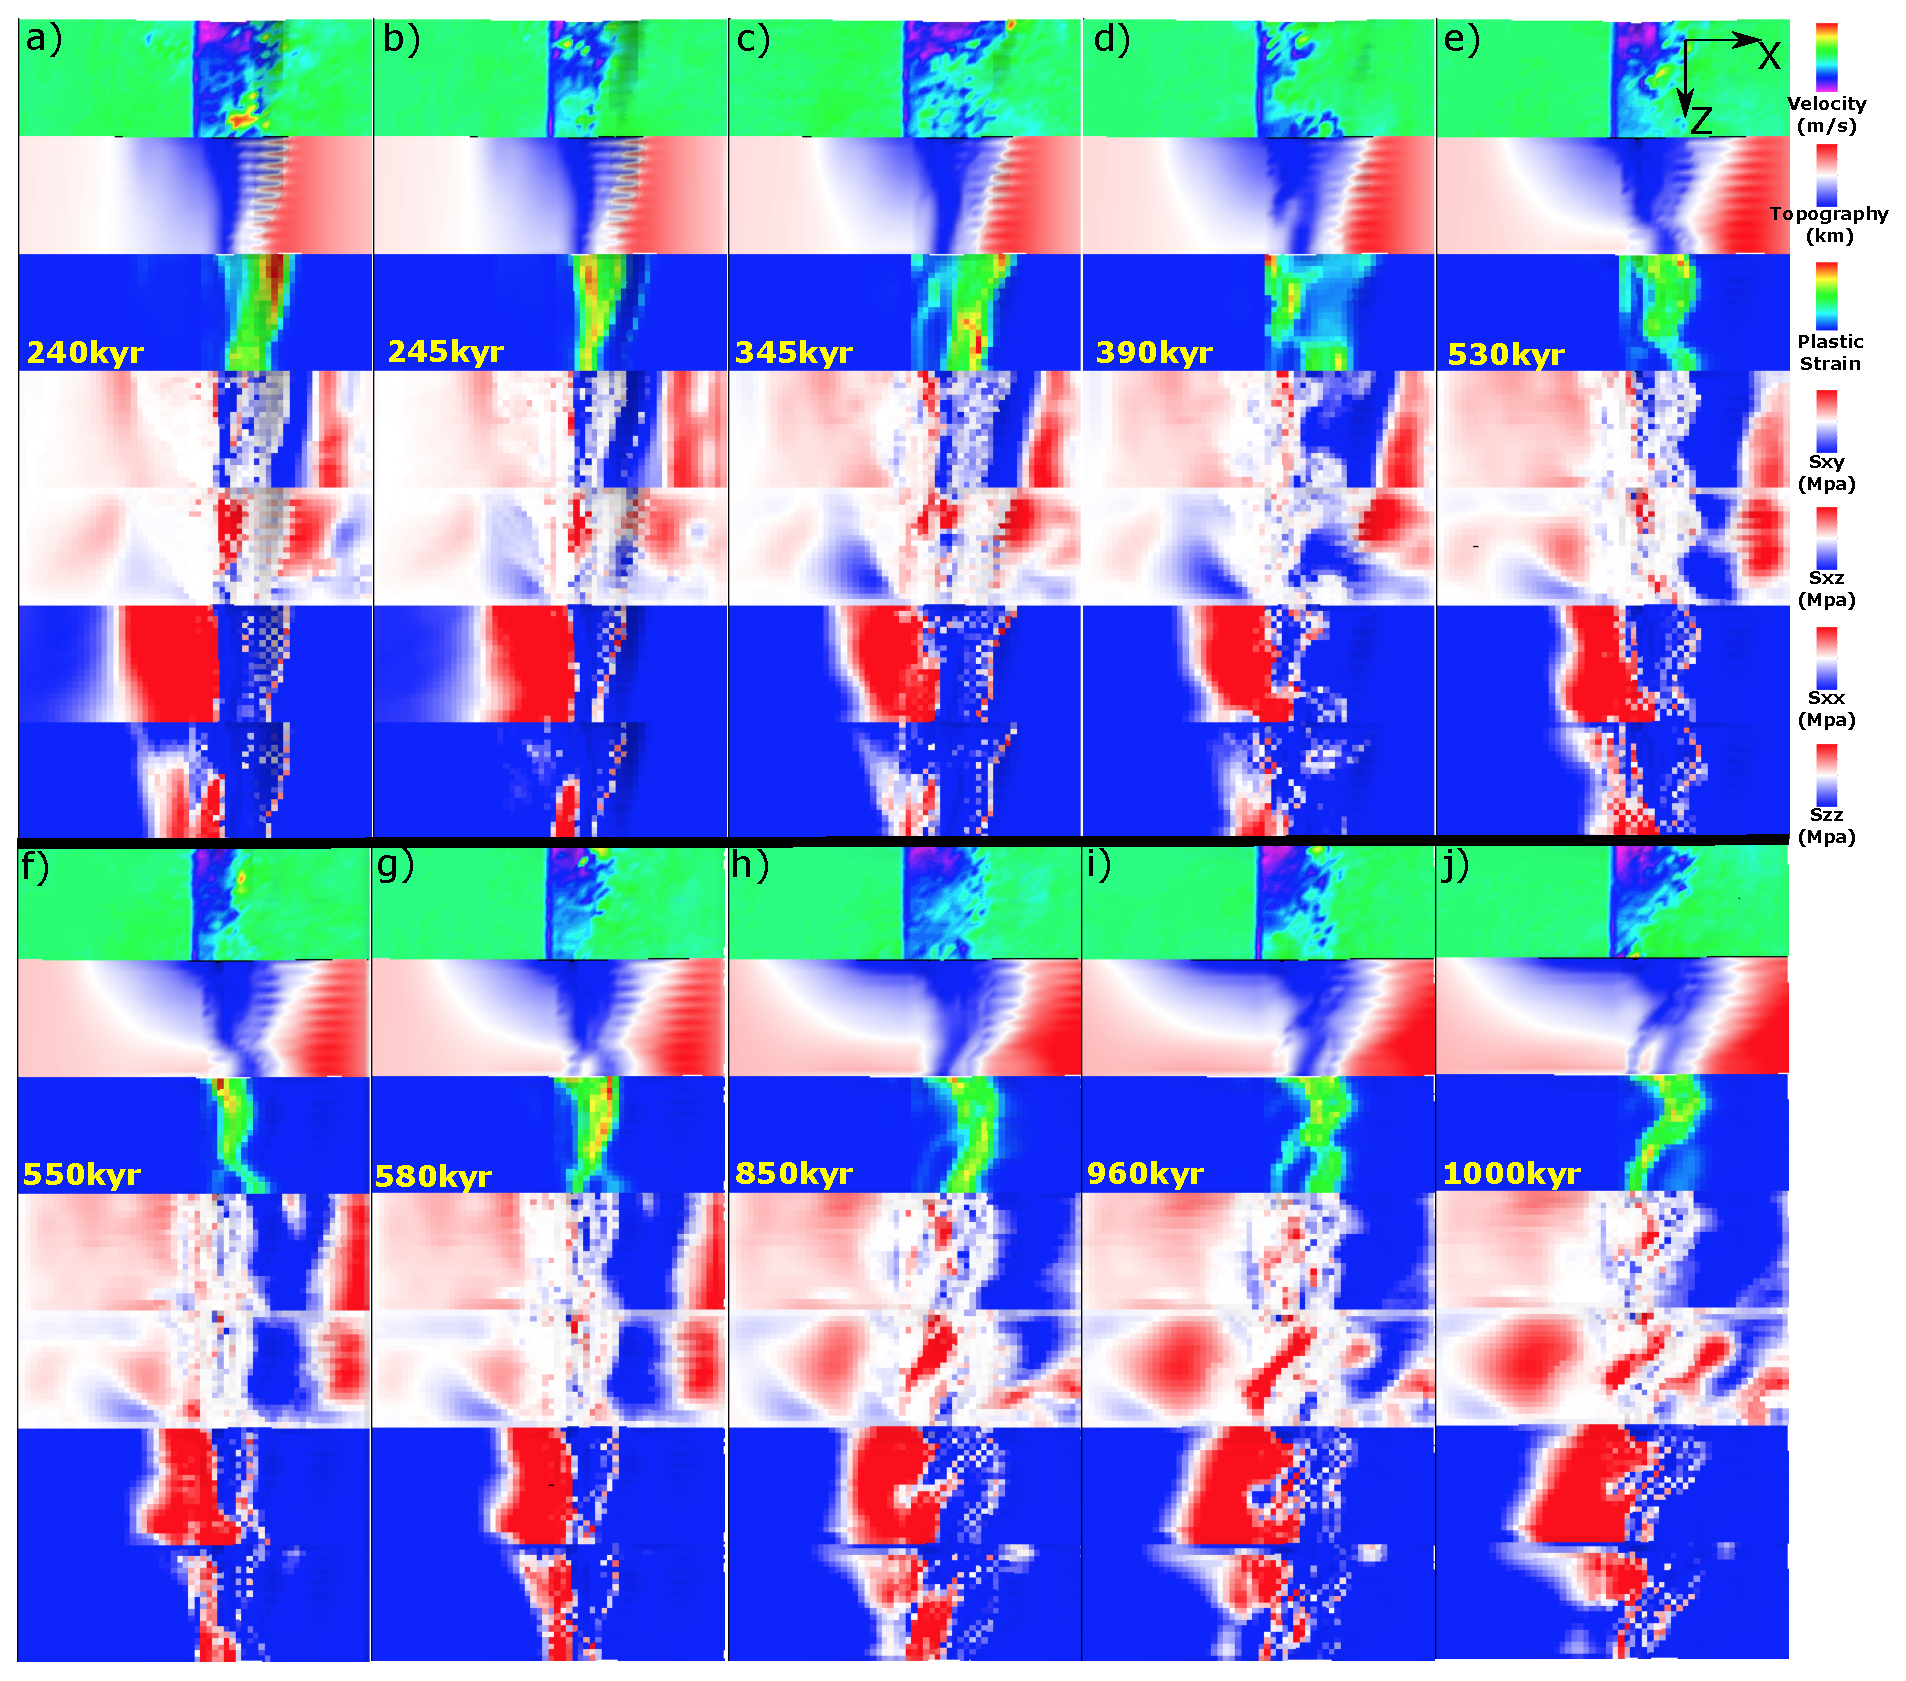
\includegraphics[width=1.0\textwidth]{./Figures/fig_Results_Weakening_5_M58SinT1_time_evolution.eps}
%  \caption{Faulting and stresses evolution (M58SinT1).}
% \label{fig_Results_Weakenging_5}
% \end{figure}

% \paragraph{M58SinT1}\label{para_M58SinT1}

% \begin{figure}[h]
%  \centering
%   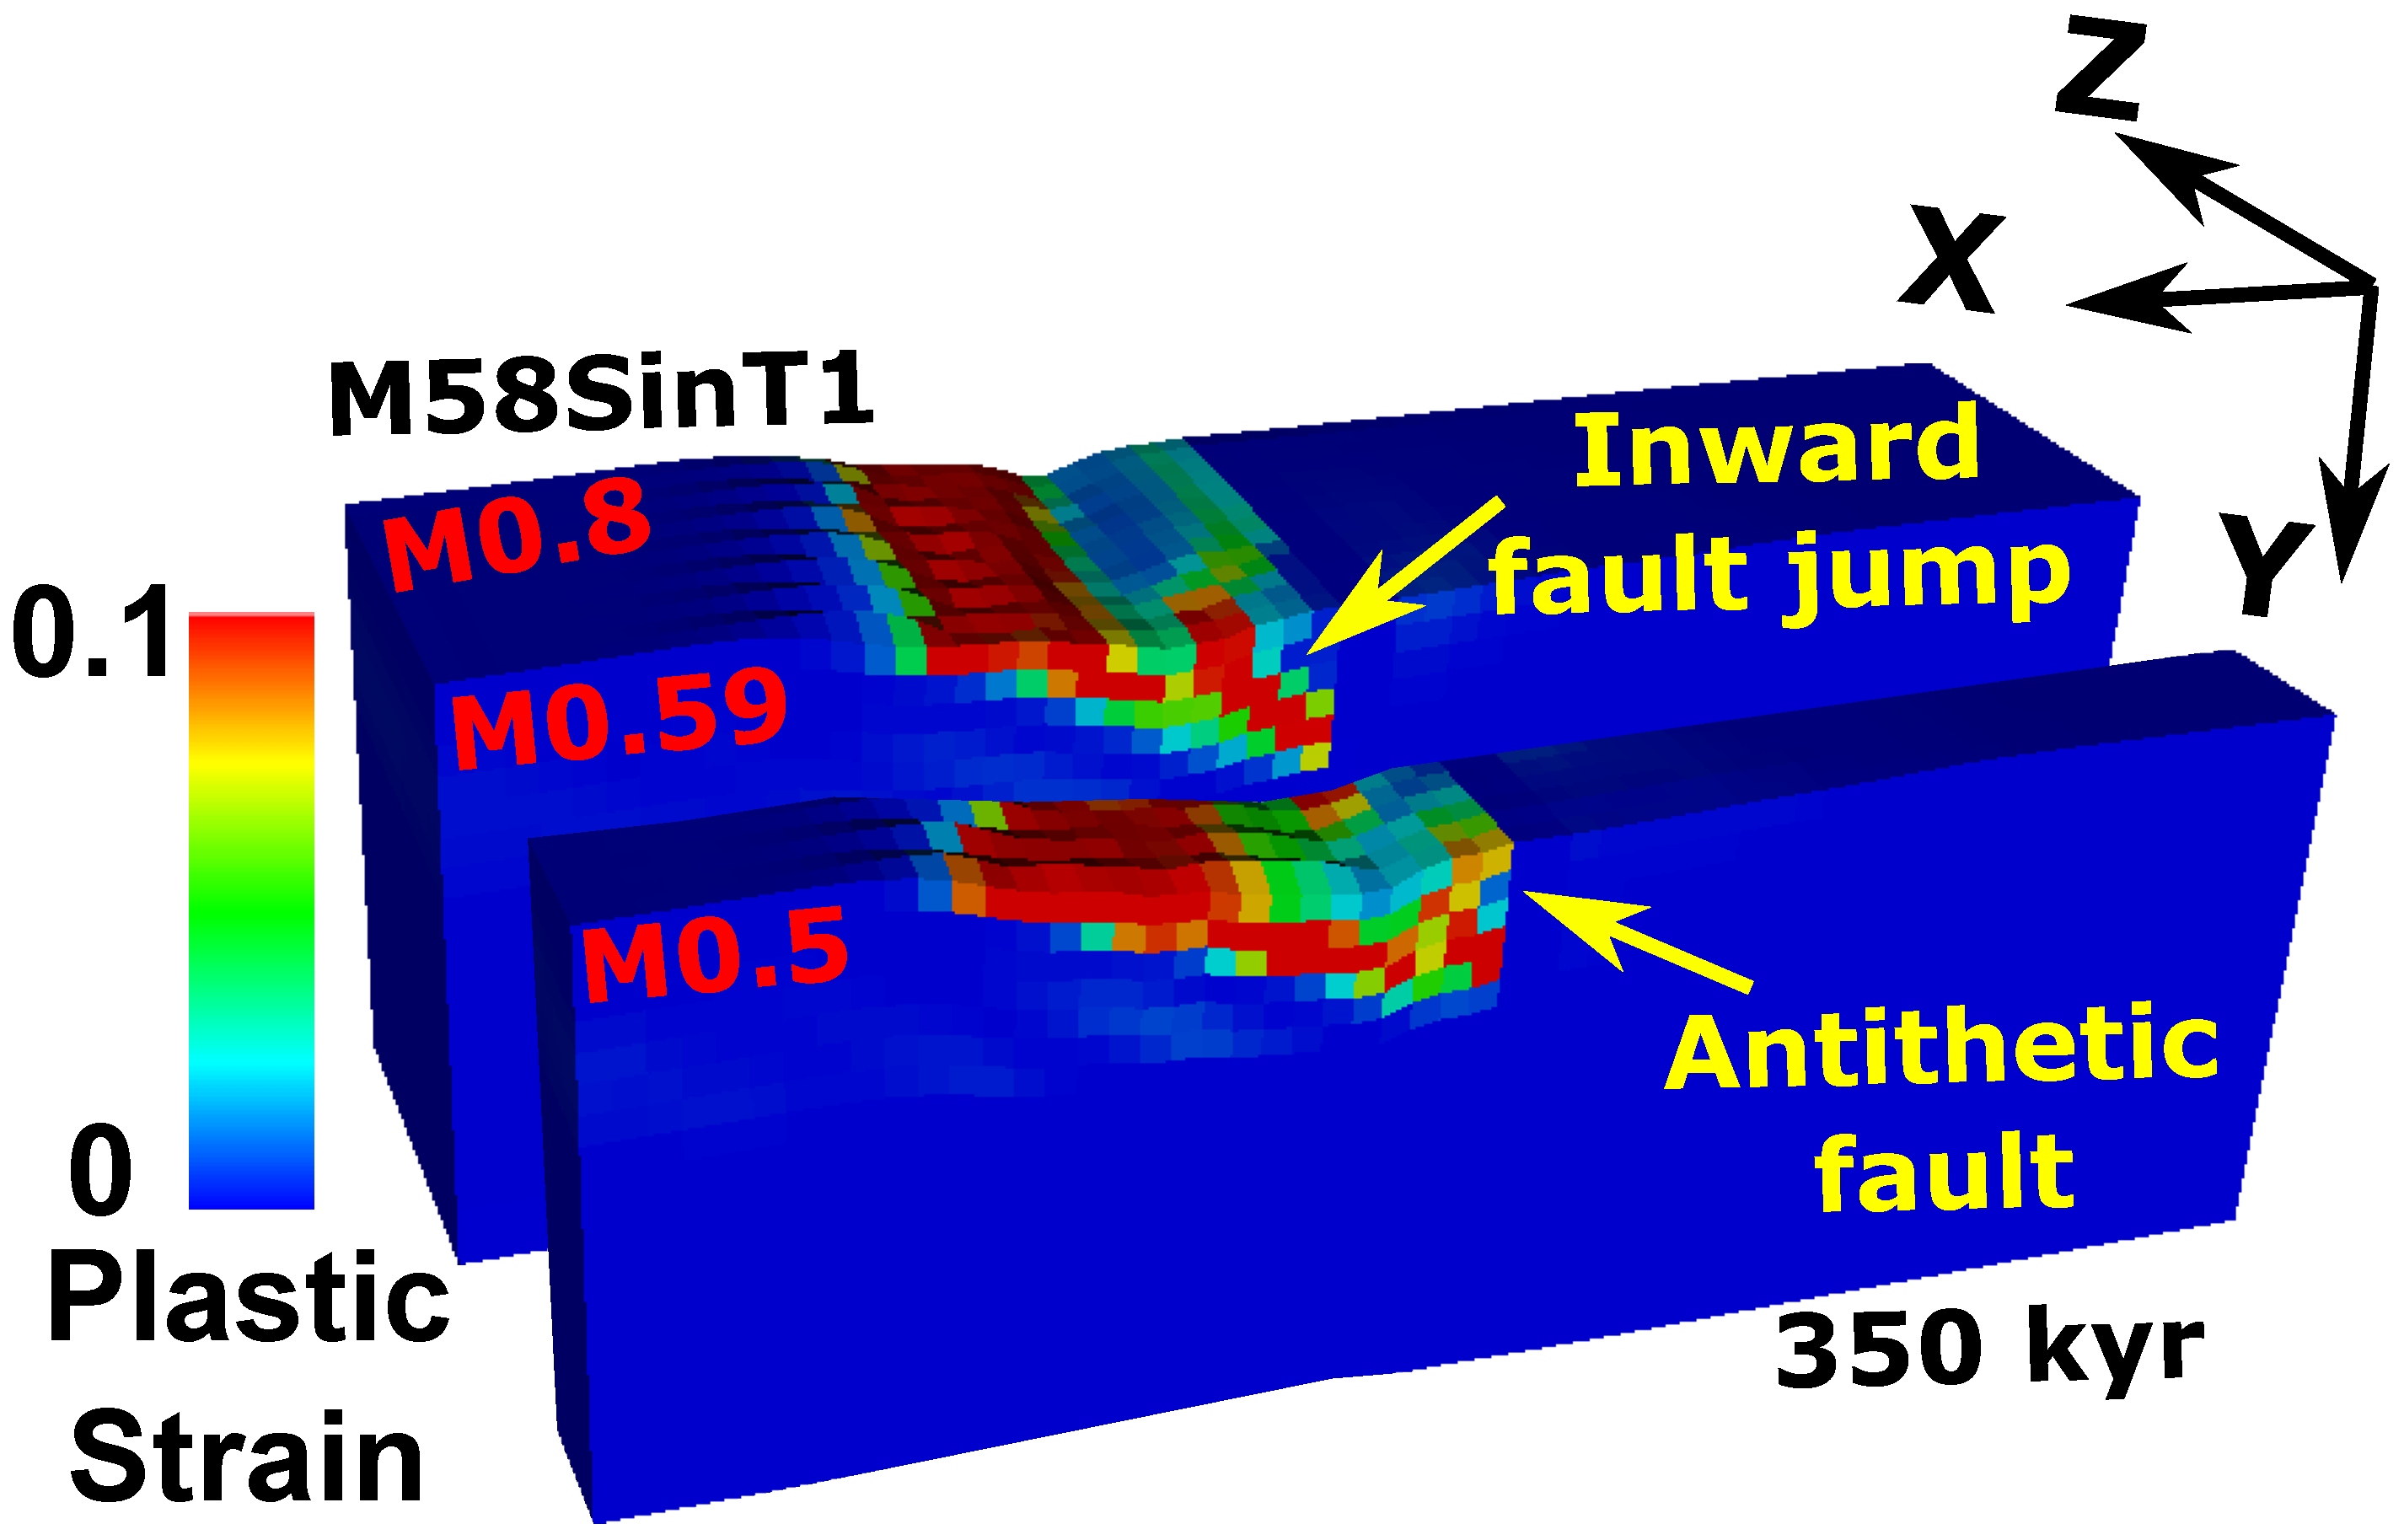
\includegraphics[width=0.6\textwidth]{./Figures/fig_Results_3_4_2_3D_Antithetic_fault.eps}
%  \caption{Plastic strain for M58SinT1 at 350 kyr.}
% \label{fig_Results_3_4_2_3D_Antithetic_fault}
% \end{figure}

% ~\\
% During the 1 Myr extension of the model M58SinT1, 10 phases of the evolution of faulting are identified (Figure~\hyperref[fig_Results_Weakenging_5]{\ref{fig_Results_Weakenging_5}.a$\sim$j}). Antithetic faults, inward fault jumps, cut-backs happens and a rider block, corrugations and mullion structures are produced.

% By 240 kyr (Figure~\hyperref[fig_Results_Weakenging_5]{\ref{fig_Results_Weakenging_5}.a}), due to fast weakening (type 1), cohesion along the termination is low. Stress $\sigma_{zz}$ takes the advantage and generates $\sim$2 km wavelength corrugations parallel to the spreading direction as the termination extends further away from the ridge axis. Between 240 kyr (Figure~\hyperref[fig_Results_Weakenging_5]{\ref{fig_Results_Weakenging_5}.a}) and 245 kyr (Figure~\hyperref[fig_Results_Weakenging_5]{\ref{fig_Results_Weakenging_5}.b}), a cut-back happens with mass wasting at the lower M side. The termination recedes toward the ridge axis during the cut-back. By 345 kyr (Figure~\hyperref[fig_Results_Weakenging_5]{\ref{fig_Results_Weakenging_5}.c}), an antithetic fault forms at the lower M side (0.5 $<$ M $<$ 0.545) with an inward fault jump happens at at ridge segment with M $\in$ (0.575, 0.635) (Figure~\hyperref[fig_Results_3_4_2_3D_Antithetic_fault]{\ref{fig_Results_3_4_2_3D_Antithetic_fault}}). 45 kyr later, the two weak zone connect to each other and take the place of the initial detachment fault at the lower M side (Figure~\hyperref[fig_Results_Weakenging_5]{\ref{fig_Results_Weakenging_5}.d}). Due to this inward fault jump, a dextral $\sigma_{xz}$ zone (blue area in the $\sigma_{xz}$ panel) forms and is bounded by the termination of the inward fault jump near the ridge axis at the lower M side and the termination of the initial detachment fault at the higher M side. By 530 kyr (Figure~\hyperref[fig_Results_Weakenging_5]{\ref{fig_Results_Weakenging_5}.e}), the termination of the inward fault jump at the lower M side evolves to a curve with its center extends further away from the ridge axis because the inward fault jump initiates at the center and starts extending away from the ridge axis earlier, however, the lower M side of the curve remains closer to the ridge axis due to the antithetic fault and the other end of the curve is also closer to the ridge axis because the fault initiates later. This curved termination at the lower M side also connects to the initial detachment fault at the higher M side which is further away from the ridge axis. Together, the curved termination is like a mirror reflected letter ``S''. This flipped ``S'' shape termination is also reflected in topography. As the curved termination at the higher M side lasts for $\sim$300 kyr since $\sim$390 kyr, following the shape, a $\sim$10 km in wavelength and $\sim$7 km in along spreading direcion mullion structure is formed (Figure~\hyperref[fig_Results_3_4_2_M58SinT1_mullion_riderBlock_inwardFaultJump]{\ref{fig_Results_3_4_2_M58SinT1_mullion_riderBlock_inwardFaultJump}}). By $\sim$680 kyr, an inward fault jump hapens at the higher M side (0.74 $<$ M $<$ 0.8). It perturbs the curved shape termination and ceases the further exhumation of the mullion structure. This inward fault jump also produces a rider block that covers the inactive detachment fault and moves off axis following the exhuming footwall of the inward jumped fault.

% \begin{figure}[h]
%  \centering
%   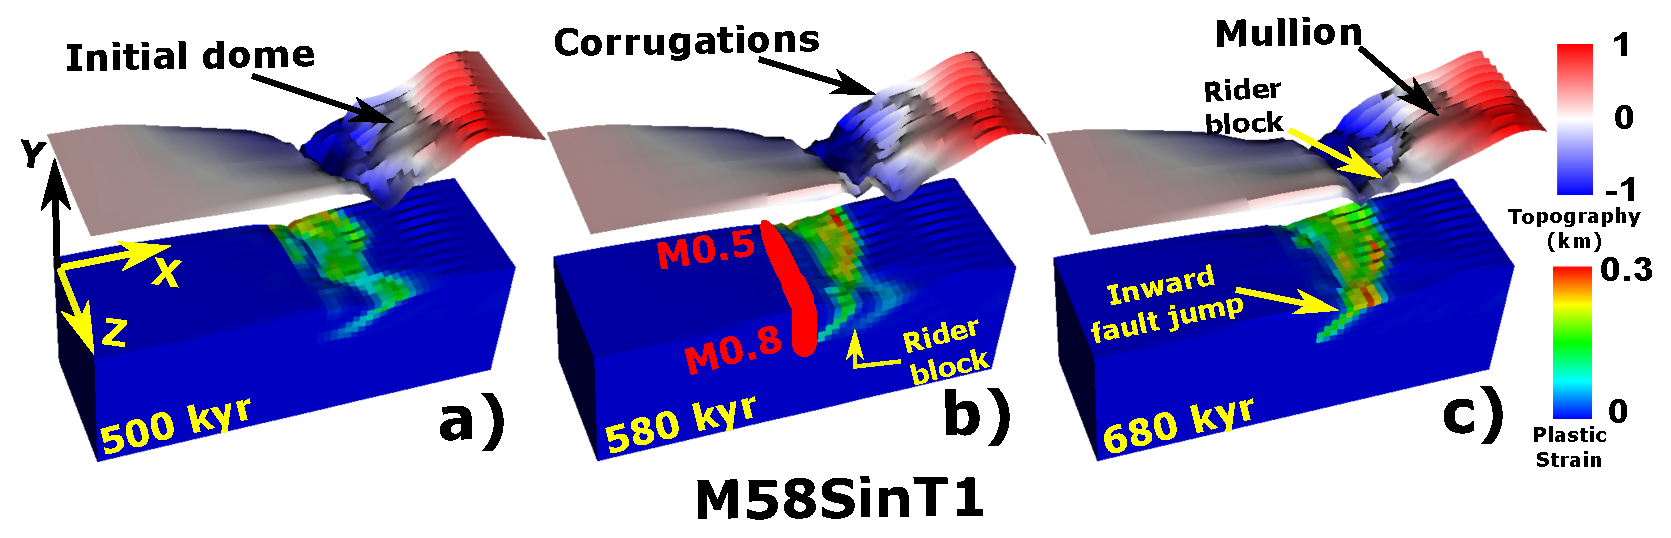
\includegraphics[width=1.0\textwidth]{./Figures/fig_Results_3_4_2_M58SinT1_mullion_riderBlock_inwardFaultJump.eps}
%  \caption{Evolution of faulting and morphologies of M58SinT1.}
% \label{fig_Results_3_4_2_M58SinT1_mullion_riderBlock_inwardFaultJump}
% \end{figure}

% Between 530 kyr (Figure~\hyperref[fig_Results_Weakenging_5]{\ref{fig_Results_Weakenging_5}.e}) and 550 kyr (Figure~\hyperref[fig_Results_Weakenging_5]{\ref{fig_Results_Weakenging_5}.f}), another cut-back happens at the lower M side (0.5 $<$ M $<$ 0.545) where a slump block with an area of $\sim$9 km$^{2}$ flows down the topography slope into the trough. Terminations recedes backward to the ridge axis. By 580 kyr, termination at the lower M side extends further away from the ridge axis due to less magma supply. Between 580 kyr and 850 kyr, due to two antithetic faults at the lower M side (M $\in$ (0.5, 0.53) $\cup$ (0.56, 0.605)), the termination at the lower M side recedes and the previous mirror reflected ``S'' shape termination evolves to a half circle curve (Figure~\hyperref[fig_Results_Weakenging_5]{\ref{fig_Results_Weakenging_5}.h}). The shape is also reflected in the topography. By 960 kyr (Figure~\hyperref[fig_Results_Weakenging_5]{\ref{fig_Results_Weakenging_5}.i})), at the ridge segment with M $\in$ (0.62, 0.665), another inward fault jump replaces the detachment fault away from the ridge axis and retreats the termination backward to the ridge axis forming two half circle curves with wavelengths of around half of the model domain in $z$-axis. A large sinistral shear zone (red region $\sim$40 $\degree$ oblique to ridge axis) is seen in the $\sigma_{xz}$ panel. The shear stress $\sigma_{xz}$ results from the inward fault jump at the center of the ridge segment that previous hanging wall changes to the footwall of the inward jumped fault and generates a offset between the old hangingwall at the lower M end and the new footwall of the inward jumped fault. By 1000 kyr, due to the along ridge coupling, the inward fault jump propogates to the higher M side (Figure~\hyperref[fig_Results_Weakenging_5]{\ref{fig_Results_Weakenging_5}.j}). 

% \paragraph{M58SinT2}\label{para_M58SinT2}

% \begin{figure}[h]
%  \centering
%   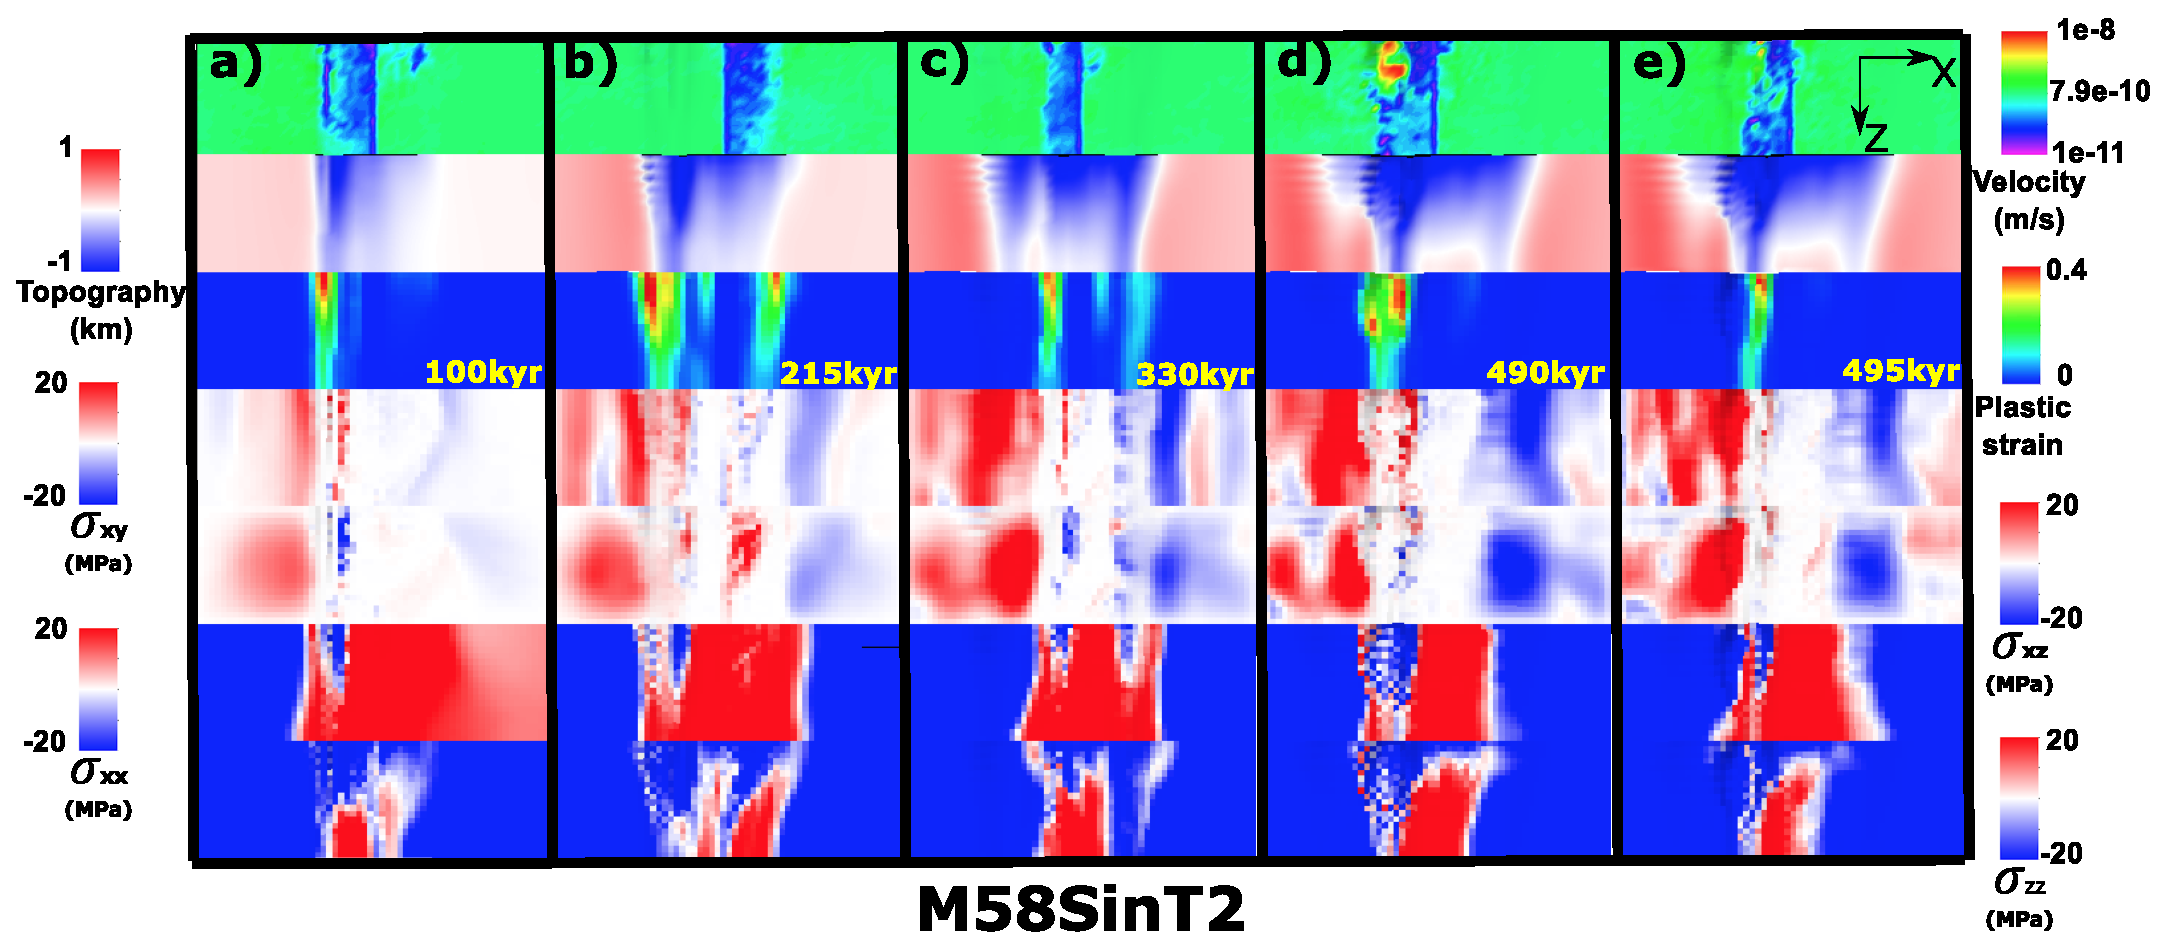
\includegraphics[width=1.0\textwidth]{./Figures/fig_Results_Weakening_6_M58SinT2_time_evolution.eps}
%  \caption{Faulting and stresses evolution of M58SinT2.}
% \label{fig_Results_Weakenging_6}
% \end{figure}

% ~\\
% As shown in Figure~\hyperref[fig_Results_Weakenging_6]{\ref{fig_Results_Weakenging_6}}, a fault initiates on the left hand side of the ridge axis (Figure~\hyperref[fig_Results_Weakenging_6]{\ref{fig_Results_Weakenging_6}.a}). The breakaway at the lower M side extends further than that of the higher M side. It takes longer time of $\sim$100 kyr to form a localized fault plane through the whole ridge segment due to the slower rate of weakening (type 2). By 215 kyr (Figure~\hyperref[fig_Results_Weakenging_6]{\ref{fig_Results_Weakenging_6}.b}), fault alternates to the conjugate plate and gradually replaces the initial one. Corrugations are only produced at the lower M side (M $\in$ (0.5, 0.62)). By 330 kyr, fault alternates again. Between 490 kyr (Figure~\hyperref[fig_Results_Weakenging_6]{\ref{fig_Results_Weakenging_6}.d}) and 495 kyr (Figure~\hyperref[fig_Results_Weakenging_6]{\ref{fig_Results_Weakenging_6}.e}), a cut-back happens with mass wasting and termination receding. A slump block of an area of $\sim$16 km$^{2}$ flows down the topography slope into the trough. With fault alternation, the shape of the median valley is no longer an hourglass. However, at the lower M side, the median valley is still wider and deeper. High frequency abyssal hills are produced at the higher M side. In addition, M58SinT2 has a fault alternation frequency of $\sim$150 kyr which is higher than that of M88ConT2. \add[XT]{Reason for this difference needs further discussion.}

% \subsubsection{M58SqrtT1 versus M58SqrtT2}

% The major difference between M58SqrtT1 and M58SqrtT2 is also whether the normal fault alternates or not.

% \paragraph{M58SqrtT1}\label{para_M58SqrtT1}

% \begin{figure}[h]
%  \centering
%   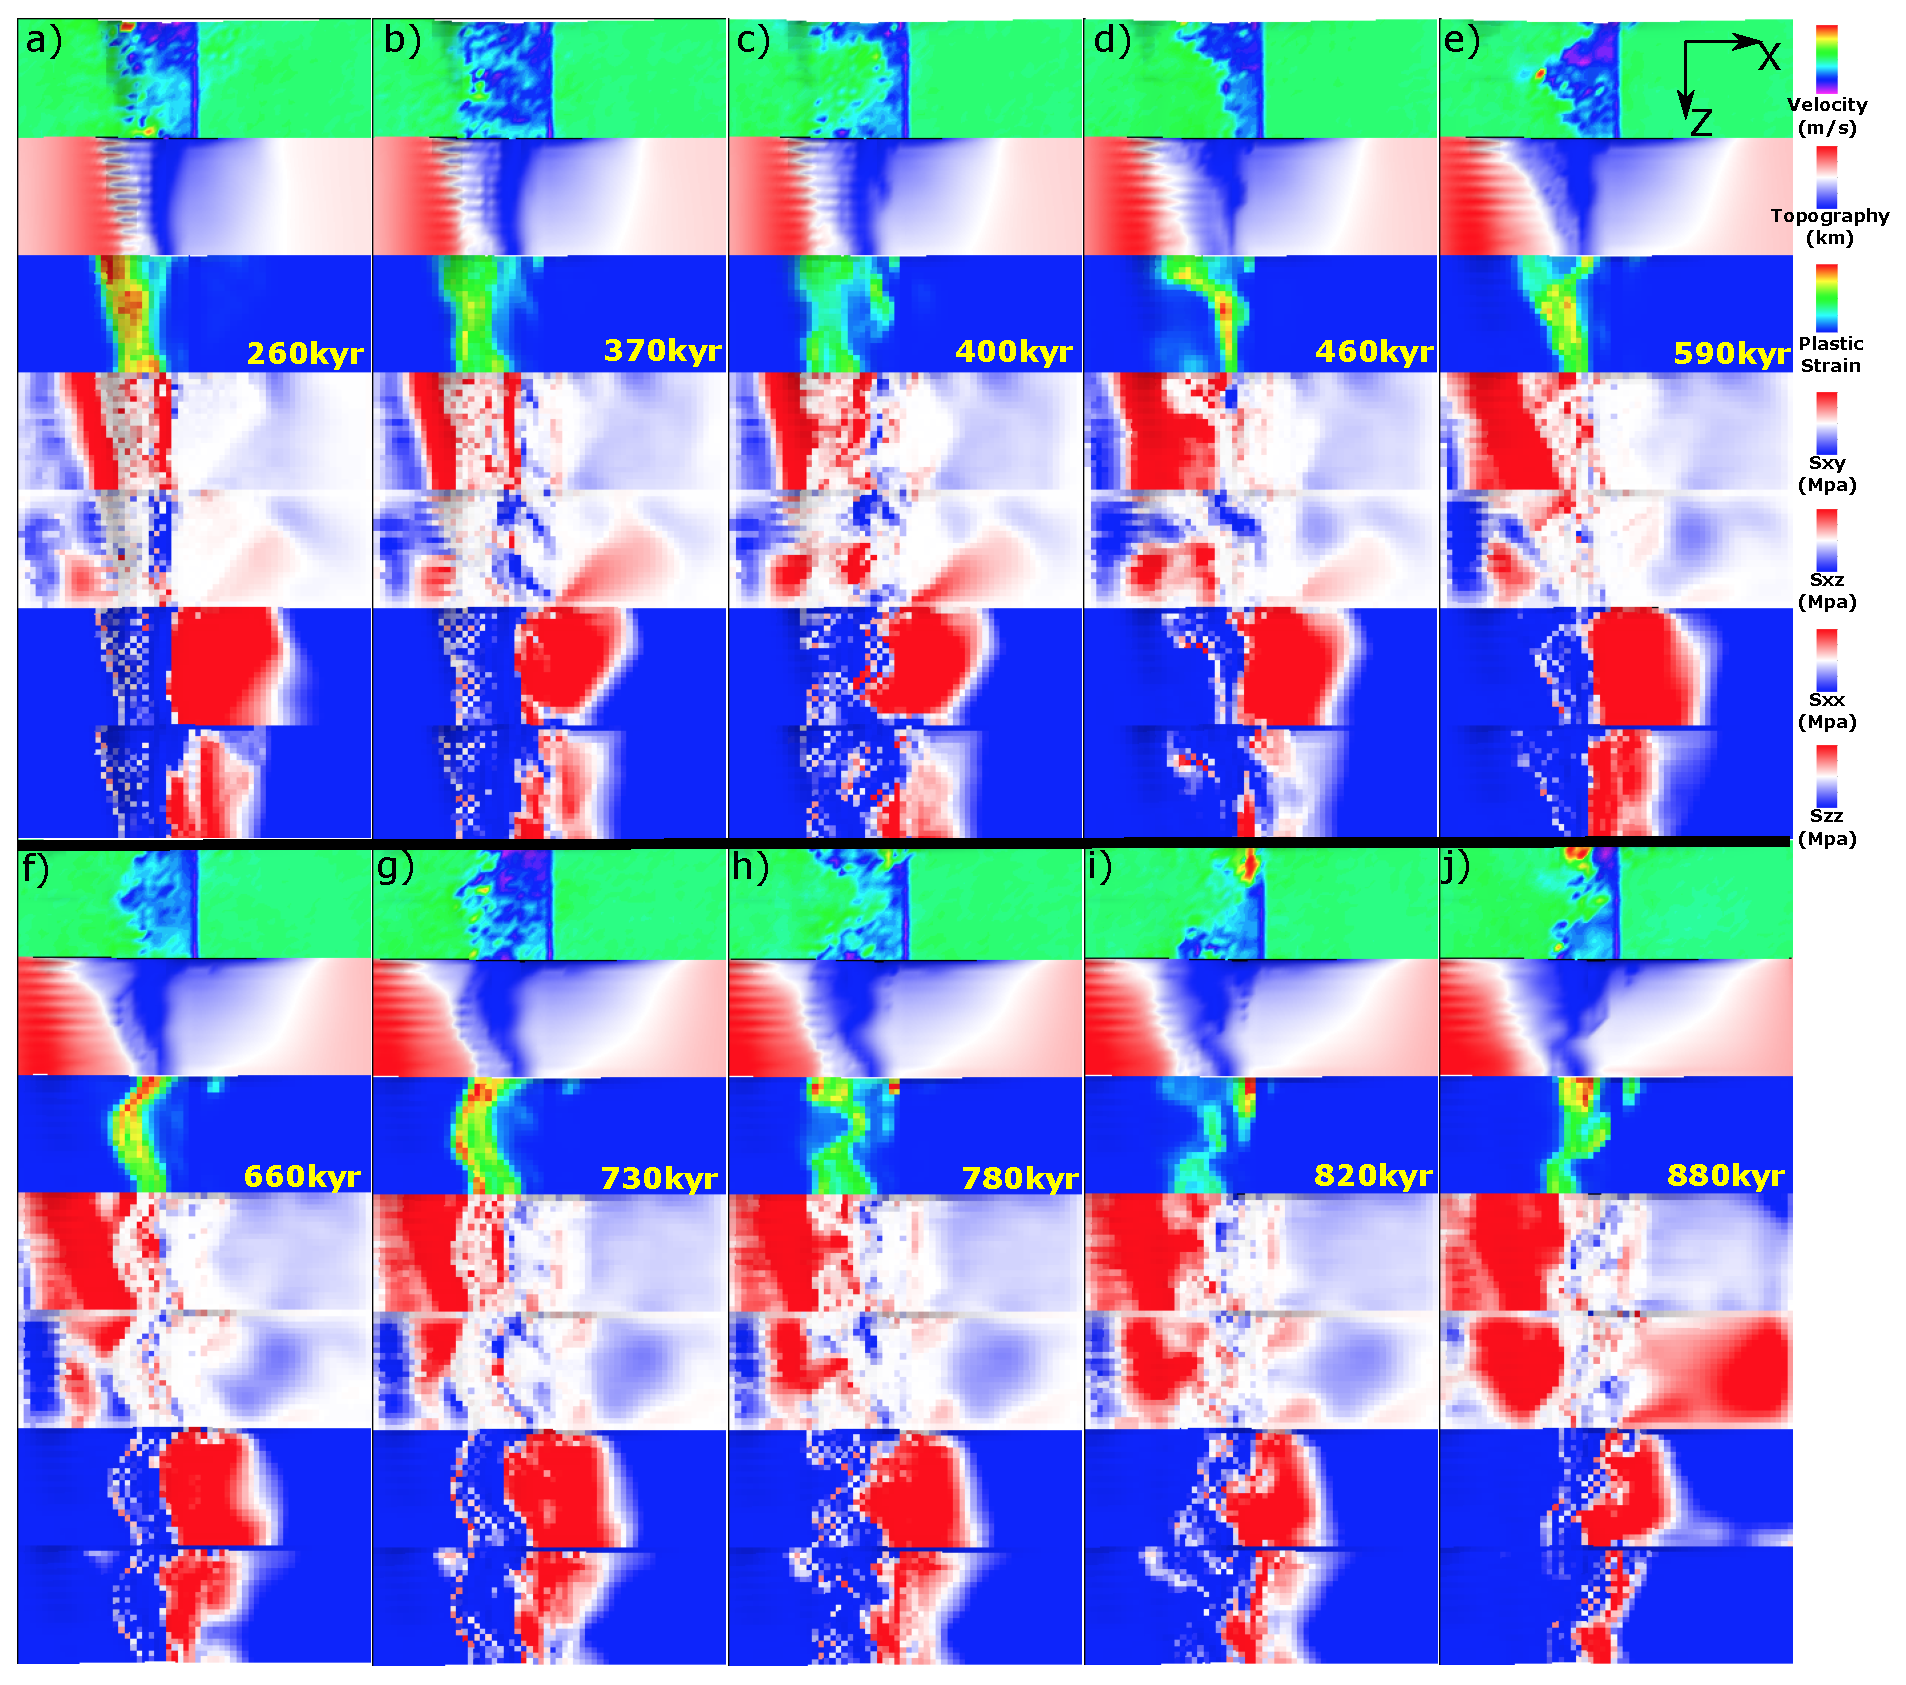
\includegraphics[width=1.0\textwidth]{./Figures/fig_Results_Weakening_7_M58SqrtT1_time_evolution.eps}
%  \caption{M58SqrtT1 (Table~\hyperref[Tab1_1]{\ref{Tab1_1}}) faulting and stress evolution with respect to time.}
% \label{fig_Results_Weakenging_7}
% \end{figure}

% ~\\
% By 260 kyr, breakaway at M $=$ 0.5 extends $\sim$5 km further away from the ridge axis than that of the higher M end (Figure~\hyperref[fig_Results_Weakenging_7]{\ref{fig_Results_Weakenging_7}.a}). Corrugations of a wavelength of $\sim$2 km \add[XT]{2 km is the correct wavelength for corrugations, change previous wrong ones of 1 km} are produced along the ridge. By 370 kyr (Figure~\hyperref[fig_Results_Weakenging_7]{\ref{fig_Results_Weakenging_7}.b}), due to larger value of $\frac{\partial M}{\partial Z}$ at the lower M side, a vertical tensile failure takes place at M $\in$ (0.5, 0.5949)\add[XT]{previous M range for Sin and Sqrt models should be revised, I used linear to calculate with respect to number of elements in Z. Start from this and the later ones are ok} . Two parallel dextral shear stress zones (blue) are seen in the $\sigma_{xz}$ panel. By 400 kyr (Figure~\hyperref[fig_Results_Weakenging_7]{\ref{fig_Results_Weakenging_7}.c}), an inward fault jump happens at where M $\in$ (0.5949, 0.7121) and it propagates to the higher M end and replaces the initial detachment fault at the higher M side by 460 kyr (Figure~\hyperref[fig_Results_Weakenging_7]{\ref{fig_Results_Weakenging_7}.d}). By 590 kyr (Figure~\hyperref[fig_Results_Weakenging_7]{\ref{fig_Results_Weakenging_7}.e}), an inward fault jump happens at the lower M side (M $<$ 0.5949) and connect with the normal fault at the higher M side replacing the initial detachment fault. An $\sim$18 km$^{2}$ triangular shape (bird's-eye view) rider block is produced at the lower M side. Termination at the center of the ridge segment extends furthest away from the ridge axis. This is because the previous inward fault jump first initiates there, so the fault starts slipping earlier and because the value of M is lower at the segment center than the higher M end. By 660 kyr (Figure~\hyperref[fig_Results_Weakenging_7]{\ref{fig_Results_Weakenging_7}.f}), as the previous inward jumped fault at the higher M side evolves, another dome is produced. There is a hint of high angle normal fault at where M $<$ 0.5949 on the conjugate plate. But it doesn't develop. By 730 kyr (Figure~\hyperref[fig_Results_Weakenging_7]{\ref{fig_Results_Weakenging_7}.g}, the termination evolves to a ``half circle'' and the shape is also seen in the topography. By 780 kyr (Figure~\hyperref[fig_Results_Weakenging_7]{\ref{fig_Results_Weakenging_7}.h}), another inward fault jump appears at the ridge segment with M $\in$ (0.6342, 0.7121) and produced a curved termination with a wavelenth of $\sim$10 km. It has the potential to create a large wavelength mullion structure. Meanwhile, at the lower M side (M $<$ 0.5949) near the ridge axis, an antithetic fault forms and propagates toward the higher M side (Figure~\hyperref[fig_Results_Weakenging_7]{\ref{fig_Results_Weakenging_7}.i}). It triggers another inward fault jump to happen at the lower M side and produces another rider block. The inward jumped fault later connects with the detachment fault at the higher M side (Figure~\hyperref[fig_Results_Weakenging_7]{\ref{fig_Results_Weakenging_7}.j}). In addition, a tensile failure shows its hint at the lower M side (M $<$ 0.6342) of the conjugate plate.

% \paragraph{M58SqrtT2}\label{para_M58SqrtT2}

% \begin{figure}[h]
%  \centering
%   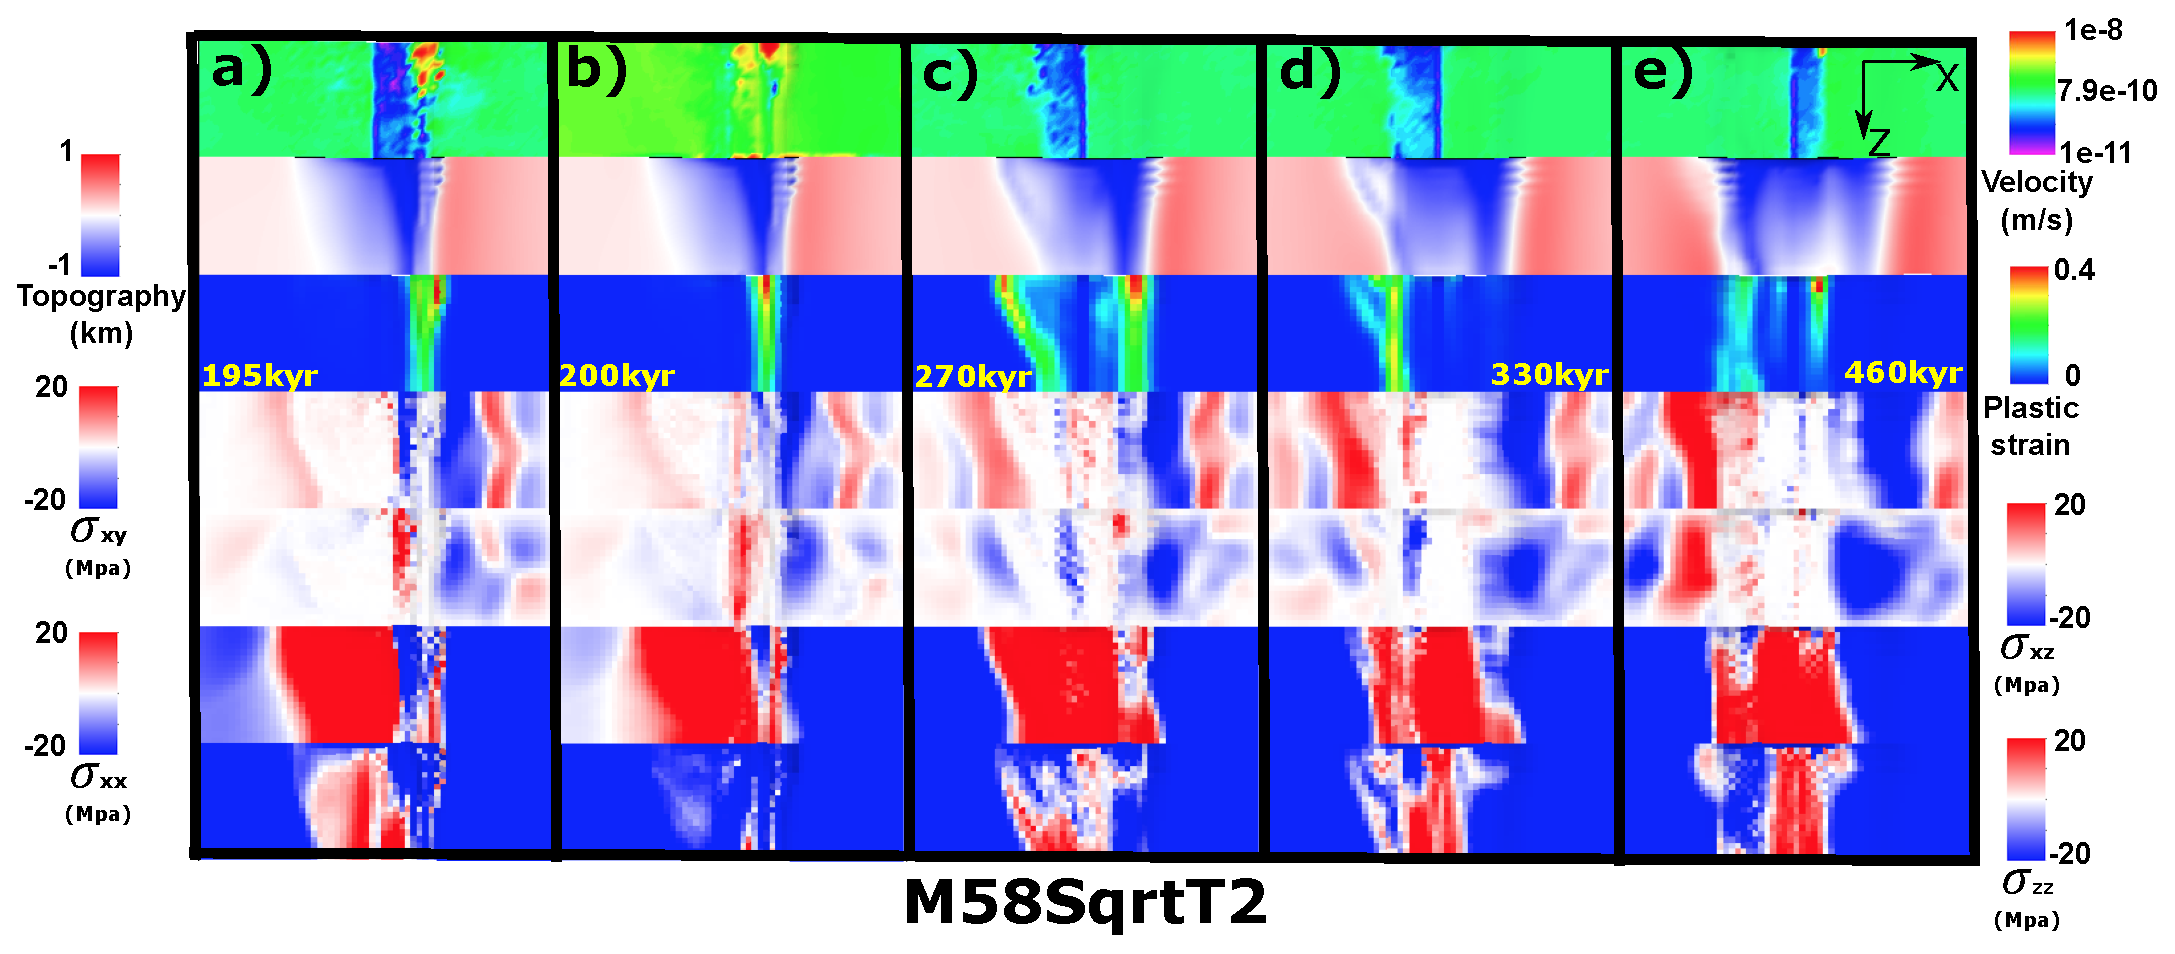
\includegraphics[width=1.0\textwidth]{./Figures/fig_Results_Weakening_8_M58SqrtT2_time_evolution.eps}
%  \caption{Faulting and stresses evolution for M58SqrtT2.}
% \label{fig_Results_Weakenging_8}
% \end{figure}

% ~\\
% By 195 kyr (Figure~\hyperref[fig_Results_Weakenging_8]{\ref{fig_Results_Weakenging_8}.a}), breakaway at the lower M side extends further away from the ridge axis. Three corrugations begin to show up due to tensile failure. Median valley on the conjugate plate is wider at the lower M side because slow weakening allows a more distributed $\sigma_{xx}$ that results in the elastic deppresion of the conjugate plate. Between 195 kyr (Figure~\hyperref[fig_Results_Weakenging_8]{\ref{fig_Results_Weakenging_8}.a}) and 200 kyr (Figure~\hyperref[fig_Results_Weakenging_8]{\ref{fig_Results_Weakenging_8}.b}),  a cut-back happens with mass wasting along the ridge and is followed by the termination retreat. By 270 kyr fault alternates (Figure~\hyperref[fig_Results_Weakenging_8]{\ref{fig_Results_Weakenging_8}.c}). The shape of the alternated fault follows the curved shape shear $\sigma_{xy}$ zone (red) as seen since $\sim$195 kyr on the left hand side of the ridge axis. By 330 kyr (Figure~\hyperref[fig_Results_Weakenging_8]{\ref{fig_Results_Weakenging_8}.d}), at the lower M side, an inward fault jump happens and takes the place of the old fault further away from the ridge axis. By 460 kyr (Figure~\hyperref[fig_Results_Weakenging_8]{\ref{fig_Results_Weakenging_8}.e}), fault alternates again to the right hand side of the ridge axis.

\subsection{Effects of the range of M variation}
Generally, M57 and M58 models create a median valley much narrower and shallower than that of M28 models.
Although the difference betweent the M ranages, 0.5-0.7 and 0.5-0.8, is seemingly small, the behaviors of M57 models and M58 ones are noticeably different.
A major difference between M57SinT1 and M58SinT1 is that the model with a greater M range (M58) shows a higher frequency of inward fault jumps, mass wasting events and connection of the offset fault zones. Also, the greater M range appears to promote the fault alternation when combined with a nonlinear M profile and a slow weakening (T2): Only the models M58SinT2 and M58SqrtT2, exhibit fault alternation.

% \subsubsection{(M28 M57 M58)SinT1}

% \paragraph{M57SinT1 versus M58SinT1}\label{M57SinT1 versus M58SinT1}

%  ~\\
%  For description of M57SinT1 evolution with respect to time, please refer to Section~\hyperref[para_M57SinT1]{\ref{para_M57SinT1}} and Figure~\hyperref[fig_Results_Weakenging_3]{\ref{fig_Results_Weakenging_3}}. For description of M58SinT1 evolution with respect to time, please refer to  Section~\hyperref[para_M58SinT1]{\ref{para_M58SinT1}} and Figure~\hyperref[fig_Results_Weakenging_5]{\ref{fig_Results_Weakenging_5}}. 
% A major difference between M57SinT1 and M58SinT1 is that the model with a greater M range (M58) shows a higher frequency of inward fault jumps, mass wasting events and connection of the offset fault zones. For M58SinT1, the inward fault jumps and antithetic faults usually replace the old ones. However, for M57SinT1, diking is not strong enough to create big enough stress perturbation along the ridge axis for inward fault jumps or antithetic faults to take the place of the original one. At the lower M side, antithetic faults only help to accommodate tensional stress which assists in maintaining a termination near the ridge axis while the termination at the higher M side gradually moves off axis. This produces an OCC with larger dome at the lower M side than that of higher M side which is opposite to the shape of the OCC produced by M58SinT1. 

% \paragraph{M28SinT1}\label{para_M28SinT1}

% \begin{figure}[h]
%  \centering
%   \includegraphics[width=1.0\textwidth]{./Figures/fig_Results_MRange_1_M28SinT1_time_evolution.eps}
%  \caption{M28SinT1 (Table~\hyperref[Tab1_1]{\ref{Tab1_1}}) faulting and stress evolution with respect to time.}
% \label{fig_Results_MRange_1}
% \end{figure}

% ~\\
% As shown in Figure~\hyperref[fig_Results_MRange_1]{\ref{fig_Results_MRange_1}}, faulting evolution is much less dynamic than that of M58SinT1. One detachment fault keeps active on the right hand side of the ridge axis. Only inward fault jump happens $\sim$540 kyr (Figure~\hyperref[fig_Results_MRange_1]{\ref{fig_Results_MRange_1}.d}). By $\sim$100 kyr (Figure~\hyperref[fig_Results_MRange_1]{\ref{fig_Results_MRange_1}.a}), breakaway at the lower M side extends $\sim$4 km further away from ridge axis than the higher M side. By 250 kyr (Figure~\hyperref[fig_Results_MRange_1]{\ref{fig_Results_MRange_1}.b}), $\sim$4 corrugations begin to evolve at the lower M side (M $\in$ (0.2, 0.5135)). By 420 kyr, at the higher M side, a hint of inward fault jump begins to show up. It delvelops into an inward fault jump by 540 kyr (Figure~\hyperref[fig_Results_MRange_1]{\ref{fig_Results_MRange_1}.d}) and propagates toward higher M side. At the lower M side (M $\in$ (0.2, 0.2939)), a tensile failure takes up part of the plate extension and helps maintain a closer to ridge axis termination than the extending termination at the region with M $\in$ (0.4724, 0.6562) (Figure~\hyperref[fig_Results_MRange_1]{\ref{fig_Results_MRange_1}.e}). The curved in termination at the lower M side produces a mullion structure.

% \subsubsection{M57SinT2 versus M58SinT2}

% For description of M57SinT2 evolution with respect to time, please refer to Section~\hyperref[para_M57SinT2]{\ref{para_M57SinT2}} and Figure~\hyperref[fig_Results_Weakenging_4]{\ref{fig_Results_Weakenging_4}}. For description of M58SinT1 evolution with respect to time, please refer to Section~\hyperref[para_M58SinT2]{\ref{para_M58SinT2}} and Figure~\hyperref[fig_Results_Weakenging_6]{\ref{fig_Results_Weakenging_6}}. A major difference is that M57SinT2 has no fault alternation while M58SinT2 has.

% \subsubsection{M28LinT1 versus M57LinT1}

% For description of M28LinT1 evolution with respect to time, please refer to Section~\hyperref[sec_M28LinT1]{\ref{sec_M28LinT1}}.

% \paragraph{M57LinT1}\label{para_M57LinT1}

% \begin{figure}[h]
%  \centering
%   \includegraphics[width=0.8\textwidth]{./Figures/fig_Results_MRange_2_M57LinT1_time_evolution.eps}
%  \caption{M57LinT1 (Table~\hyperref[Tab1_1]{\ref{Tab1_1}}) faulting and stress evolution with respect to time.}
% \label{fig_Results_MRange_2}
% \end{figure}
% ~\\
% As shown in Figure~\hyperref[fig_Results_MRange_2]{\ref{fig_Results_MRange_2}}, between 160 kyr (Figure~\hyperref[fig_Results_MRange_2]{\ref{fig_Results_MRange_2}.a}) and 162.5 kyr (Figure~\hyperref[fig_Results_MRange_2]{\ref{fig_Results_MRange_2}.b}), a cut-back happens. The corrugations have a relatively high amplitude. Due to less M variation (0.2), the along ridge offset in breakaways is smaller. The median valley almost has a constant width along the ridge. By 350 kyr (Figure~\hyperref[fig_Results_MRange_2]{\ref{fig_Results_MRange_2}.c}), a tensile failure happens at the region with M $\in$ (0.5, 0.61) and generates a linear topography low. Another shorter tensile failure at the higher M side (M $>$ 0.64) helps maintain a high angle normal fault near the ridge axis. By 430 kyr (Figure~\hyperref[fig_Results_MRange_2]{\ref{fig_Results_MRange_2}.d}), the tensile failure at the lower M side (M $<$ 0.52) is responsible for the retreat of the termination. While at where M $\in$ (0.54, 0.59), the termination extends further away from the ridge axis. This curved termination results in a ``dog bone'' shape topography as seen at 640 kyr (Figure~\hyperref[fig_Results_MRange_2]{\ref{fig_Results_MRange_2}.e}) and is also responsible for the large dextral shear (blue) stress $\sigma_{xz}$. By 705 kyr (Figure~\hyperref[fig_Results_MRange_2]{\ref{fig_Results_MRange_2}.f}), an inward fault jump happens and replaces the original detachment fault at the higher M side with a length of $\sim$15 km. This inward jumped fault connects with the detachment fault at the lower M side. The new ``L'' shape termination is responsible for the topography seen at 1000 kyr (Figure~\hyperref[fig_Results_MRange_2]{\ref{fig_Results_MRange_2}.h}). The termination at the higher M side soon catches up the further extended termination at the lower M side due to the presence of a tensile failure.
       
% \subsubsection{M28SqrtT1 versus M58SqrtT1}

% For description of the evolution of M28SqrtT1, please refer to Paragraph~\hyperref[para_CutBack]{\ref{para_CutBack}}. For description of evolution of M58SqrtT1, please refer to Paragraph~\hyperref[para_M58SqrtT1]{\ref{para_M58SqrtT1}}. Generally the faulting evolution for M58SqrtT1 is more dynamic with several inward fault jumps, antithetic faults, connection between offseted faults along the ridge while M28SqrtT1 is simpler with only two cut-backs.

% \subsubsection{M57SqrtT2 versus M58SqrtT2}

% For description of evolutio of M58SqrtT2, please refer to Paragraph~\hyperref[para_M58SqrtT2]{\ref{para_M58SqrtT2}}.

% The major difference between M57SqrtT2 and M58SqrtT2 is that only M58SqrtT2 has fault alternation.

% \paragraph{M57SqrtT2}

% \begin{figure}[h]
%  \centering
%   \includegraphics[width=0.8\textwidth]{./Figures/fig_Results_MRange_3_M57SqrtT2_time_evolution.eps}
%  \caption{M57SqrtT2 (Table~\hyperref[Tab1_1]{\ref{Tab1_1}}) faulting and stress evolution with respect to time.}
% \label{fig_Results_MRange_3}
% \end{figure}

% ~\\
% For M57SqrtT2, six small scale \note[EC]{how small is small and how big is big?} mass wasting events occur at 282.5 kyr, 290 kyr, 365 kyr, 452.5 kyr, 482.5 kyr and 540 kyr respectively. As shown in Figure~\hyperref[fig_Results_MRange_3]{\ref{fig_Results_MRange_3}}, the fault keeps on the left hand side of the ridge axis. By 200 kyr (Figure~\hyperref[fig_Results_MRange_3]{\ref{fig_Results_MRange_3}.b}), an inward fault jump begins to evolve and takes the place of the initial fault. As the fault evolves, a stage of discontinuous abyssal hill is produced at the lower M side (Figure~\hyperref[fig_Results_MRange_3]{\ref{fig_Results_MRange_3}.c}). The fault propagates toward the higher M side and cuts through the plate by $\sim$245 kyr (Figure~\hyperref[fig_Results_MRange_3]{\ref{fig_Results_MRange_3}.d}) when corrugations at the lower M side are produced. Between 365 kyr (Figure~\hyperref[fig_Results_MRange_3]{\ref{fig_Results_MRange_3}.e}) and 367.5 kyr (Figure~\hyperref[fig_Results_MRange_3]{\ref{fig_Results_MRange_3}.f}), a cut-back happens. By 490 kyr (Figure~\hyperref[fig_Results_MRange_3]{\ref{fig_Results_MRange_3}.g}), an antithetic fault begins to evolve and terminates the old fault. It then develops into a vertical tensile failure at 540 kyr (Figure~\hyperref[fig_Results_MRange_3]{\ref{fig_Results_MRange_3}.h}). \add[XT]{for M57SqrtT2, the topography since 200 kyr uplifted, I suspect ther might be some runtime error for this model. Consider to abandon this model and if possible, rerun it. }
\fi
% Between the \iffalse and \fi are the short version of the three effects of M ranges, functional forms and two type weakening rates. 
